% Root File for a UC Dissertation / Thesis
% UCD thesis class: c/o Shwaine <shwaine@shwaine.com>
%
% modified by Dylan Beaudette, 2006,2010
% modified  and source uploaded to github by Alex Mandel, 2014
% Source code available at http://github.com/wildintellect/ucdthesis
\documentclass[12pt,oneside,draft]{ucdthesis}
%\documentclass[10pt,twoside,final]{ucdthesis}
% \documentclass[10pt,oneside,final]{ucdthesis}

\usepackage[final]{graphicx}
% TODO: this makes strange things happen in the header...
% this is the version that grad studies wants
% \documentclass[11pt,oneside,final]{ucdthesis}

% when we are giving people drafts, use more of the page:
\usepackage[letterpaper,
    inner=1.0in,
    outer=2.25in,
    top=1.25in,
    bottom=2.0in,
    marginparsep=0.25in,
    marginparwidth=1.0in]{geometry}

\setlength{\footskip}{1.25in}
\setlength{\headsep}{1.25in}
\setlength{\headheight}{15pt}
% need this for the \foreach command
\usepackage{tikz}
\usetikzlibrary{calc,shapes,arrows,positioning}

% Turn on single spacing with \ssp.
% Turn on double spacing with \dsp.
% By default, your dissertation is double spaced, as is required by UCD.
\usepackage{setspace}
\makeatletter
\let\@currsize\normalsize
\makeatother
\setstretch{1.86}

% spacing in figures and tables and their captions can be
% changed here (\ssp for single-space, empty for same as surrounding
% text); for this to work, the command \figsp has to be included
% in every figure and table right after the \begin{figure}
% \def\figsp{\ssp}
%\def\figsp{}


% useful for drafts
% line numbers:
% http://www.ctan.org/tex-archive/help/Catalogue/entries/lineno.html
%
%\usepackage{lineno}

%
% SVN integration
%
% \usepackage{svnkw}

\usepackage{calc}

% customized headers
%
% http://www.ctan.org/tex-archive/help/Catalogue/entries/fancyhdr.html
\usepackage{fancyhdr}

\newlength{\myoddoffset}
\setlength{\myoddoffset}{\marginparwidth + \marginparsep}

\rhead{\input{git-header}}
\chead{\textbf{---DRAFT---}}
\lhead{}
\cfoot{---\thepage---}
\fancyheadoffset[R]{\myoddoffset}
\fancyfootoffset[R]{\myoddoffset}

\fancypagestyle{plain}{%
    \fancyhf{}
    \fancyfoot[C]{---\thepage---}
    \fancyhead[C]{\textbf{---DRAFT---}}
    \fancyhead[R]{\input{git-header}}
\fancyheadoffset[R]{\myoddoffset}
\fancyfootoffset[R]{\myoddoffset}
}
\fancypagestyle{frontmatterstyle}{%
    \fancyhf{}
    \fancyfoot[C]{---\thepage---}
    \fancyhead[C]{\textbf{---DRAFT---}}
    \fancyhead[R]{\input{git-header}}
\fancyheadoffset[R]{\myoddoffset}
\fancyfootoffset[R]{\myoddoffset}
}

% a better verbatim environment: c/o Pete Dirac
% use like this:
%   \begin{Verbatim}[fontsize=8]
%       foobar
%    \end{Verbatim}
% \usepackage{fancyvrb}


% more flexible math support
\usepackage{amsmath}

% allow some pages to be landscape
\usepackage{lscape}

% more flexible definition of table environments
\usepackage{ctable}

%need this for \includegraphics{}
\usepackage{graphicx}

%enable the listings package specifically for including programming code
\usepackage{listings}

%Special hack to make code listings not break pages, fyi they must be short then
\usepackage{float}
\floatstyle{plain} % optionally change the style of the new float
\newfloat{Code}{H}{myc}

%test alternative to listings package minted which requires the python pygments package
%minted was installed to latex by hand
%\usepackage{minted}

% TODO: use the new subfig package instead
% http://www.ctan.org/tex-archive/macros/latex/contrib/subfig/
%
%use this to put figures side by side
\usepackage{subcaption}

 % PDF links --- > breaks with some bibliography entries
% \usepackage{hyperref}

% nice looking, parenthetical references
%\usepackage[sorting=nyt,natbib=true,citestyle=authoryear,bibstyle=authoryear,maxnames=3,refsection=chapter]{biblatex}
%\usepackage[sorting=nyt,natbib=true,citestyle=authoryear,bibstyle=authoryear,maxnames=3,refsection=chapter]{biblatex}

\usepackage[utf8]{inputenc}
\usepackage[english]{babel}

\usepackage{natbib}
\renewcommand\bibname{References}
\def\newblock{\hskip .11em plus.33em minus.07em}
\bibliographystyle{abbrvnat}
\setcitestyle{authoryear, open={(},close={)}}
%%\usepackage{chapterbib} % incompatible with biblatex
%\bibliography{dissertation}
%\defbibheading{bibliography}{%
%	\section{References}
%	}
%	
%% bibliography can be single-spaced for UC thesis format
%\appto{\bibsetup}{\ssp}
%	

%make the index
% \usepackage{makeidx}
% \makeindex

% custom colors
\usepackage{color}
% make a color for comments
\definecolor{MyDarkBlue}{rgb}{0,0.08,0.45}

% customized captions with bold label and small, italic text
% table captions are located above tables
% http://www.kronto.org/thesis/tips/custom-captions.html
% http://www.ctan.org/tex-archive/macros/latex/contrib/caption/
% does this have any effect?
%\usepackage{caption}
% \renewcommand{\captionfont}{\small\itshape}
%
\usepackage[hypcap,font=singlespacing]{caption}
%\usepackage{subcaption}
% modern method for setting up captions\
\captionsetup{margin=10pt,font=small,labelfont=bf}
%
% fix so that table captions have correct spacing
\captionsetup[table]{position=top}



% %
% %  fit more material on the page:
% %
%
% reset some float-controlling parameters
\renewcommand{\floatpagefraction}{0.8}	% require fuller float pages

% N.B.: floatpagefraction MUST be less than topfraction !!
\renewcommand{\topfraction}{0.9}	% max fraction of floats at top
\renewcommand{\bottomfraction}{0.8}	% max fraction of floats at bottom


% PDF formatting options, indexing, hyperlinking, with control over link style
%Set PDF Metadata
\title{Performance of a Novel Virtual Environment for Cockpit Evaluation}
\author{Richard D. Joyce}
\makeatletter
\usepackage[pdftex,
            pdfauthor={\@author},
            pdftitle={\@title},
            %pdfsubject={Subject},
            %pdfkeywords={Comma, List, Keywords},
            %pdfproducer={Latex with hyperref, or other system},
            %pdfcreator={pdflatex, or other tool}
            ]{hyperref}
\makeatother
\hypersetup{
    % driver=pdftex,
    final=true,
	colorlinks=true,
	urlcolor=blue,
	linkcolor=blue,          % color of internal links
    citecolor=blue,        % color of links to bibliography
    filecolor=magenta
}

%Use an additional package to make bookmarks point to the top to tables, figures and listings
\usepackage[all]{hypcap}

%Alex's customizations
\usepackage{indentfirst} %Indents first paragraph of chapter
\usepackage{datatool} %Allows import of csv and other data-tables
\usepackage{varwidth}
\usepackage{color}
\usepackage{rotating}
%\AtEveryBibitem{\clearfield{month}} %Cleaner references without month being printed

\graphicspath{{./figures/}{./plots/}}

\newcommand{\tablepath}{./tables/}

\makeatletter
\newcommand{\includetable}[1]{%
  \@ifundefined{tablepath}{%
    \InputIfFileExists{#1}{}{}%
  }{%
    \InputIfFileExists{\tablepath/#1}{}{\InputIfFileExists{#1}{}{}}%
  }
}
\makeatother

\usepackage{booktabs}
\usepackage{dcolumn}
\newcolumntype{.}{D{.}{.}{-1}}
% more space between table rows
\renewcommand{\arraystretch}{1.2}

\usepackage{csquotes}
\renewcommand\mkbegdispquote[2]{\leavevmode\llap{``}}
\renewcommand\mkenddispquote[2]{#1''#2}

\usepackage{todonotes}
\newcommand{\tinytodo}[1]
{\todo[size=\small]{\linespread{1.0}%
\selectfont%
#1%
\par
}}

\usepackage{mathtools}

\usepackage{enumitem}

\usepackage{multirow}

\usepackage{nameref}

%\usepackage[maxfloats=58]{morefloats}

%%% Document Portion:
\begin{document}


%
%% Title, Front Matter, and Abstract:
% Skip for draft
% % Declarations for Front Matter

% MS Thesis = 0, Phd Dissertation = 1
\isdissertation{1}

% electronic submission? Paper only = 0, Electronic = 1
\iselectronic{1}

\title{Performance of a Novel Virtual Environment for Cockpit Evaluation}
\author{Richard D. Joyce}

% Choices are September, December, March, June
\degreemonth{March}
\degreeyear{2018}
%More examples DOCTOR OF PHILOSOPHY
\degree{Doctor of Philosophy}

\chair{Stephen K. Robinson}
\othermembers{Ron A. Hess,Michael Feary} %comma separated list of committee not including chair
\numberofmembers{3} % size of committee

\prevdegrees{M.S (University of California at Davis) 2013}
\prevdegrees{B.S (Columbia University) 2009}

%Your Graduate Group
\field{Mechanical and Aerospace Engineering}
\campus{Davis}


% add the abstract here

% Their are two abstracts. One that is published externally from your
% dissertation, and one that is internal. Of course, the text of the
% abstract will be the same. So, we define a macro to hold the body of our
% abstract.
% at 345 words - With electronic filing there is no longer a word limit

\newcommand{\myabstract}{
put the abstract here
}


%Not required for electronic submission, you will need to print your other abstract page 2x and hand them in.
% Here is the first, external, abstract.
%\begin{abstract}
%	\myabstract
%	\abstractsignature
%\end{abstract}

\begin{frontmatter}
\maketitle

% A copyright page is optional. If you have one, it must immediately
% follow the title page. For more information about the copyright page
% see the UCD's Office of Graduate Studies web site.
% \copyrightpage

% dedication (optional), remove comment markers to use
%\begin{dedication}
%\null\vfil
%{\large
%\begin{center}
%xxxx
%\end{center}}
%\vfil\null
%\end{dedication}



\tableofcontents
\listoffigures
\listoftables

% Here is the second, internal, abstract.
% Update: Melissa Danforth 2006
% Inline abstract is now part of front matter according to coordinator
    \newpage
    \begin{inlineabstract}
		%Only enable small if you're trying to make it fit.
		%\begin{small}
		\myabstract
		%\end{small}
    \end{inlineabstract}

%Acknowledgments (optional)
\begin{acknowledgments}
    John Karasinski, mostly.
\end{acknowledgments}

%Preface (optional)
% \chapter*{Preface}
% \addcontentsline{toc}{chapter}{Preface}
% \input{preface}


\end{frontmatter}


%
% the chapters
%

% set page style:
% make the chapter and section smaller, chapter and section numbers are removed
% fancyplain will keep the page numbers at the bottom of all pages
%\pagestyle{fancyplain} %Note the \fancyplain command !!!
%\renewcommand{\chaptermark}[1]{\markboth{\small{#1}}{}}
%\renewcommand{\sectionmark}[1]{\markright{\small{#1}}{}}

\pagestyle{fancy}

% TODO: this is only for draft copies !!
% start line number printing
%


\tableofcontents

\chapter{Introduction}

\section{Overview}
\label{overview}

The motivation for the research presented stems from the design of complex human-machine interfaces, particularly cockpits for spacecraft and high performance aircraft.
A common problem is that the design (or modernization) of a cockpit will go into flight before evaluation pilots are completely satisfied with the design process, due to time and budget concerns.
The remaining deficiencies of the cockpit design are expected to be overcome through additional crew training.
These deficiencies represent a cost throughout the lifetime of the vehicle in training, and ``unknown'' deficiencies of the human-machine system are often discovered too late in accident reports.
To address these issues, we have designed and prototyped a virtual environemnt which allow pilot evaluations to occur earlier and more frequently in the design process.
The aim of our system is to add the immersion and interactivity benefits of a more functionaly simulator to the non-functioning geometric mockup.
The mockup, which is used in the early stage of the design process, can now be used for more extensive cockpit evaluations with this system installed on top.
This brings the accompanying benefits of a simulator with the benefits of early stage design mockups: faster and more drastic redesign iterations.
Additionally, the use of the hand tracker allows for a more thorough examination of the movement of evaluation pilots than is typically possible.

The prototype system, called the ``Rapidly Reconfigurable Research Cockpit'', consists of a virtual reality (VR) headset, an optical hand tracking device, and 3D printed cockpit surfaces (Figure \ref{fig:intro_r3c}).
The VR head-mounted display (HMD) provides a virtual view of the cockpit environment.
A challenging aspect of immersive VR simulations, however, is to provide a sense of touch.
%an appropriate tactile feel of the objects being interacted with (in our case, the instruments of a cockpit).
We provide this by using 3D-printed instruments co-located with the virtual environment, a technique commonly called ``passive haptics''.
The instruments remain inert and non-functioning in the real world, but appear fully functional in the virtual world presented to the user.
They can be modelled to the exact shape of a cockpit instrument being designed, and printed within a matter of hours.
The user can interact with the virtual cockpit (i.e.\ pressing buttons) with the use of an optical based hand tracker, which measures the position of the pilots' hand.
Their hand position is used to determine if the user is activating a button, as well as to display the hand in the virtual world.
Normally, the use of an HMD blocks the view of one's own limbs, so not only does the hand tracker provide the input of the button presses, but provides the user with visual feedback of their hand.
%Measurements from the hand tracker are used to display the essential visual feedback of hand position in the virtual world, as normally the use of an HMD blocks the view of one's own body.

This prototype has been the technical base for the research performed in this work.
The three main tracks of the research can be summarized in these aims:


\begin{enumerate}
    \item Create a virtual reality system with passive haptics and hand tracking that allows for evaluation of early design cockpits (Chapter \ref{chap:proto}).
    \item Validate the technical approach and evaluate the performance of subjects in the virtual reality environment with passive haptics (Chapter \ref{chap:pointing} and \ref{chap:haptics}).
    \item Evaluate the use of the prototype in a mock design evaluation study to determine the differences in standard performance metrics and subject feedback from using our system (Chapter \ref{chap:design_exp})
\end{enumerate}

Three experiments with human subjects have been performed and are reported on to support these aims.
The first experiment (Chapter \ref{chap:pointing}) asked subjects to repeatedly target one of four buttons on the panel under different conditions, testing differences between real versus virtual world as well as passive haptics versus no passive haptics (mid-air reaching).
We recorded time to completion and accuracy to the button center.
%It was found that the virtual world caused a slight but significant degradation in time for the reaching movement, but no significant change in accuracy.
%The accuracy requirement is more important for our application of safety-critical human-machine interfaces, where accuracy requirements often prevail over movement time.
The second experiment (Chapter \ref{chap:haptics}) had subjects perform a Fitts' Law task in different conditions to further characterize the difference between using passive haptics and mid-air reaching.
%The recorded 3D hand trajectory data will also be used to develop the metric for Aim 3 (which is being called the ``task familiarity'' metric or model in this report).
%By using the Fitts' circle for Experiment 2, we can use the Fitts' throughput as a truth measure of familiarity to train and test the model upon.
Additionally, this experiment had a more extensive subject survey to collect the opinions of the subjects, especially their opinion on the differences between passive haptics and mid-air reaching.
The final experiment (Chapter \ref{chap:design_exp}) compared the performance of the R3C prototype as a design evaluation tool against an evaluation using a more traditional simulation.
Subjects were split into two groups, one using the R3C, the other a touchscreen simulator.
Two instrument designs were presented to each subject and they were asked to perform the same task on both.
Afterwards, their comments about the two designs were collected.
Performance measures of the task were also recorded and analyzed.
The goal of the experiment was to determine where subject feedback and performance may differ between an evaluation study using R3C and one using a touchscreen.
The differences found were described and discussed.


\section{Literature Review}
\label{literature-review}

To frame this research, this section will summarize relevant previous work.
The first few sections deal with virtual reality: different haptic environments and evaluation of virtual environments.
Next input device evaluation research such as Fitts' Law is discussed, highlighting work that has been performed evaluations in virtual environments.
The final section discusses the trajectory models that we propose using as% a basis for extension into a ``task familiarity''
metric.

\subsection{Virtual Tactile Environments}
\label{virtual-tactile-environments}

One of the challenges of virtual environments has been presenting the user with a tactile sensory input that matches the visual sensory inputs they are experiencing.
Many haptic glove products have been created that attempt to simulate this with motor vibrations.
Since they are attached to your body, they cannot provide any external stopping force, so the simulation can break down when interacting with rigid objects.
Another technique is using a stylus mounted to a 6-DOF actuator that can simulate external forces.
These have been used for many studies with the application of surgical tasks, when a tool would be used in the real scenario as well.
The focus of this work is the idea of \emph{passive haptics}, whereby the tactile environment is recreated to provide the sense of touch, including external forces.
 The disadvantage is that the tactile environment cannot dynamically change during the simulation.
Some researchers have attempted to create robotic passive haptics (McNeely \& others, 1993; Tachi, Maeda, Hirata, \& Hoshino, 1994), which use a robotic arm to deliver the appropriate tactile experience to the user as they reach into the virtual world.
This approach quickly becomes complicated and expensive.
Others have tried approaches to morph the virtual world to adapt to a generic passive haptic device (Kohli, 2009; Kohli, Whitton, \& Brooks, 2012), which can work only for small discrepancies.
Fortunately, the adaptability during a simulation of the passive haptic environment is not a requirement for the use case of a pilot evaluating a new cockpit interface.
We still retain the ability to quickly change the environment in between simulation sessions via 3D printing new parts.

The first appearance of work similar to ours was by Schiefele et al.  (1998) in Germany, which also used a head-mounted display (HMD) to replace the visuals of a flight simulator (though technology has drastically changed in HMD's since their work).
They recreated only the positions of the panels with a flat plate and then used a magnetic hand tracker for reading the pilot input.
A short usability study was presented, and they found that users could activate switches, knobs and dials in less time with the physical panel than without (i.e.\ reaching into mid-air).
\tinytodo{not sure if have more aviation refs}

Previous work with passive haptics, though limited, have shown it to provide benefits.
Insko (2001) investigated the impact of passive haptics on generic virtual environments.
It was found that the passive haptics increased the sense of presence felt by users.
An experiment had two groups complete a maze in a virtual environment, one group with passive haptics on boundaries, and one without.
After training the passive haptic group bumped into far fewer obstacles than the group without.

Borst and Volz (2005) created a ``mixed'' haptic virtual environment, whereby they combined an active haptic glove with a passive haptic panel.
The panel provided the stopping force and depth location of the interface, while the glove haptics provided the finer details of the buttons, switches and dials.
They compared subjects performing tasks on the panel using the glove by itself (no panel), the passive haptics by itself, as well as their mixed condition.
They found the glove by itself consistently performed worse than the other two, but overall no significant difference existed between passive haptics and their mixed haptics.

\subsection{Virtual Environment Evaluation}
\label{virtual-environment-evaluation}

It is notoriously hard to quantify the effectiveness of a virtual environment (VE).
One can report on quantitative measures of the virtual reality (VR) setup such as latency, field of view, resolution and others, but in the end the only useful measure is whether the user finds the virtual environment convincing.
This can also change depending on the user -- one user could find a VE convincing while another finds it intolerable.
The effectiveness of a VE is often linked to the sense of \emph{presence}, defined ``as the subjective experience of being in one place or environment, even when one is physically situated in another'' (Witmer \& Singer, 1998).
Sheridan (1992) argued that presence is a subjective sensation that necessitates a subjective measure.
It is important to quantify this as increased presence has been shown to improve task performance (Youngblut \& Huie, 2003).
Two of the more popular post-questionnaires that have been developed are the Presence Questionnaire (PQ) (Witmer \& Singer, 1998) and the Slater-Usoh-Steed (SUS) questionnaire (Slater, Usoh, \& Steed, 1994).
The former (PQ) consists of 32 questions that cover various factors of presence such as sensory, control, distraction and realism.
The SUS questionnaire consists of only 6 questions and is focused on the feeling of presence.
 Nystad \& Sebok (Nystad \& Sebok, 2004) found the PQ to be more sensitive to technology and interaction methods, while the SUS fits better to the definition of presence.
This suggests PQ may be better suited for our work when comparing between conditions, but SUS could be useful as a general evaluation of the overall system.
The increased presence with passive haptics found by Insko (2001) is an important finding we aim to replicate for our virtual environment.
\tinytodo{expand on why presence is important}

We also hypothesize that our system will reduce the amount of arm fatigue experienced by the operator compared to a mid-air pointing virtual environment (i.e.\ no tactile workstation present).
This common phenomenon in virtual environments is often called gorilla arms, as people feel that their arms are too heavy to support after prolonged use reaching out into the void.
A measure of this arm fatigue is not included in the standard presence questionnaire.
The literature does not contain a large volume of experiments that measure arm fatigue.
 Qualitative measures include the Likert scale, NASA Task Load Index (NASA TLX), the ISO-9241-9 ``Assessment of Comfort and Fatigue'' and the Borg scales (RPE and CR10).
The Borg CR10 performs favorably to the other scales for measures of exertion (Grant et al., 1999).
Recently, a quantitative approach has been proposed that uses optical tracking of the arm and wrist which validated well against a Borg CR10 scale (Hincapié-Ramos, Guo, Moghadasian, \& Irani, 2014).
Adapting their software to our system would be out of scope (and requires more upper-limb measurement than we are currently capable of) but the validation against the Borg CR10 scale is promising.

\subsection{Workload}

\todo{this section}

\subsection{Input Device Evaluation}
\label{input-device-evaluation}

For decades one of the most important empirical models in the Human-Computer Interface (HCI) community has been Fitts' Law.
The basis of the model is a method to predict the movement time of a user towards a target.
Using just the size and distance to the target, the average movement time can be accurately predicted after emperically determining the model parameters.
It has been used to evaluate new input devices to determine how fast a user can move to a target (e.g.\ mice, trackballs, joysticks), as well as a guideline for interface designs (ensuring that target areas are the right size).
A summary of the field is presented here, with notable contributions and similar work following.
Fitts' Law used in the context of virtual environments and our work is then discussed.

\subsubsection{Fitts' Law}
\label{fitts-law}

Paul J.\ Fitts (1954) originally reported on his experiments of targeted reaching movements between varying target sizes, and compared the linear trend he discovered to information theory models.
He postulated that the entire control system of the human, from motor control to visual and proprioceptive feedback, can process information at a certain maximum rate, and the bandwidth of the channel must be derivable from the physical parameters of the target.
Fitts' adapted Shannons' Theorem (Shannon, 1949) from information theory for the bandwidth of a channel in the presence of a signal and noise.
The distance to the target (\emph{D}) is considered the signal, and the width of the target (\emph{W}) is considered to be the noise (Figure \ref{fig:intro_fitts}).
This analogy allowed Fitts' to create a formula for the \emph{index of difficulty} (\(\text{ID}\)) of a target:

\begin{equation}
    \mathrm{ID} = \log\left(\frac{2D}{W}\right)
    \label{eq:intro_id}
\end{equation}

It was found experimentally that the index of difficulty is linearly correlated to \emph{movement time} (MT), the time taken to move between the start and the target.
This leads to the equation that is now known as Fitts' Law:

\begin{equation}
    \mathrm{MT} = a + b \cdot \mathrm{ID}
\end{equation}
where \emph{a} and \emph{b} are the parameters of the linear regression, which are determined experimentally.
A typical experiment consists of subjects performing movements to a range of targets with varying index of difficulty, and recording their movement time.
The data is then fit to a linear regression.

Since its original formulation, refinements to the model have focused on the formula for index of difficulty, \(\text{ID}\), and the definition of its dependencies, width and distance.
Crossman (1957) suggested a very important refinement called the adjustment for accuracy.
This provides a correction to the \(\text{ID}\) to compensate for the task which is actually performed by the subject as opposed to the task that was asked to be performed.
For example, if a subject is presented with two large targets close together (\emph{D} \textless{}\textless{} \emph{W}), then he/she tends to aim towards the inner edges of the targets instead of the center, effectively using a much smaller target width.
The adjustment for accuracy replaces the width, \(W\), with the \emph{effective width}, \(W_{e}\).
The basis for this adjustment is that the information theory basis for Fitts' Law expects that the ``noise'' of the target width induces a 4\% error rate (I.\ S.\ MacKenzie, 1992).
If more or less than 96\% of the target hits are successfully within the target, then the target width is adjusted with the adjustment for accuracy to fit the target error rate of 4\%.
Motor tasks have been shown to be a Gaussian distribution (Crossman \& Goodeve, 1983; Welford, 1968; Woodworth, 1899), thus 96\% of target endpoints will be within 4.133 standard deviations (\(\sigma\)).

\begin{equation}
W_{e} = 4.133\sigma
\end{equation}

It is recommended to calculate the effective width for each subject in each condition as it is sensitive to both between and within subject variability.
The effective width can then be used to calculate an \emph{effective index of difficulty}, \(\text{ID}_{e}\).
The effective width described here is for one dimensional targets, but there are extensions to 2D targets as well (Murata, 1999).

The form of the logarithmic term in the index of difficulty equation (Eq.\ \ref{eq:intro_id}) has encountered some debate over the years.
Fitts did not describe the reasoning for including the factor of two in his original formulation, and Welford (1968) suggested a modification that provided a better fit for low values of index of difficulty.
The Welford modification simply adds
\begin{equation}
    \mathrm{ID} = \left( \frac{D}{W} + 0.5 \right).
\end{equation}
A more recent variation noted by I.S.\ MacKenzie (1989) suggests that by comparing to Shannons' Theorem, as Fitts originally proposed as the theoritical basis for his work, then the form should be,
\begin{equation}
    \mathrm{ID} = \left( \frac{D + W}{W} \right) = \left( \frac{D}{W} + 1 \right)
\end{equation}
which has been widely adopted in literature as the Shannon's Formulation.
The mathematical structure of this formulation, unlike the original equation, will not produce a negative index of difficulty with real, positive dimensions.


The first use of Fitts' Law in the human-computer interface (HCI) community was with Card et al.\ (1978), comparing the use of a mouse, joystick and keys for text selection.
This led to an extensive use of Fitts' Law in the HCI field, both as a way to evaluate input devices and a design law for user interfaces.

Best practices of using Fitts' Law have been developed, and the standard ISO-9241-9:2000 (International Organization for Standardization, 2000) provided guidelines for the use of Fitts' Law in evaluation of input devices.
Most notably, it was suggested to use the ISO-9241 ``Fitts' circle'' for evaluations of 2D tasks (Figure \ref{fig:intro_fitts_circle}).
This input pattern has been adopted widely in literature, and provides a standard for comparing across studies.

Soukoreff \& I.S.\ MacKenzie (2004) present a review of the best practices for designing and performing a Fitts' law experiment, including the use of the Shannon Formulation and the ISO-9241 ``Fitts' circle''.
They also advise the use a large range of ID values, ideally from 2 to 8 bits.

%Many experiments achieve this by varying distance and width, but Guiard (2009) points out the inconsistency of designing for a range of ID based on two factors, and shows that by holding one fixed lowers the regression error, while reducing experiment complexity.
%Wobbrock (2011) provided an independent validation of this, showing that significant effects remained when retroactively removing the varying diameter of targets.

When used to evaluate input devices, the metric of comparison is often \emph{throughput}.
Throughput (TP) is defined as the index of difficulty (ID) over the movement time (MT).
\begin{equation}
    \mathrm{TP} = \frac{\text{ID}}{\text{MT}}
\end{equation}
The units of throughput are bits per second, and it represents the information capacity of the input device.\tinytodo{add importance sentence}
A higher throughput indicates that the human is able to convey more information through one input device versus another.
One of the advantages of using throughput is that it combines speed and accuracy requirements through the use of the index of difficulty.
Throughput has been validated to be invariant to subjects prioritizing speed or accuracy (I.  S.  MacKenzie \& Isokoski, 2008).

The debate on which form and refinement of Fitts' Law is the best to use continues to this day (Drewes, 2010; Hoffmann, 2013), and this work will not attempt to settle this debate.
%\tinytodo{rewrite this}However, the understanding of the origin of Fitts' Law, best practices and the many forms of the equations will greatly influence the design and success of the experiments performed.
Since no form of the equations have been rejected outright in the literature, it is recommended to perform analysis with all versions and note if any significant differences in major conclusions result (Soukoreff \& MacKenzie, 2004).

\subsubsection{Dimensionality of Fitts' Law}\label{dimensionality-of-fitts-law}

Throughout the Fitts' Law literature one of the differences between experiments is how many dimensions the subjects can move (or move their cursor).
There are two dimensionalities to consider when discussing Fitts' Law experiments: the dimensionality of the targets or task, and the dimensionality of the movement.
A 1D task means the targets are aligned along a single axis, whereas a 2D task has them located on a plane (such as the Fitts' circle in Figure \ref{fig:intro_fitts_circle}).
The dimensionality of the movement refers to how many dimensions the subjects need to move when moving between the targets.
For example, the original Fitts' Law task was a 1D task as the targets were varied in width along the movement direction, but sufficiently long in the perpindicular dimension, removing that dimension as a variable.
The movement however was effectively 2D, as the subjects could (and needed to) lift up from the table to move between targets.

The popularity of Fitts' Law in the HCI field has led many researchers to focus on the use of Fitts' Law on a 2D computer screen controlled by a mouse.
This is a 2D task, with a constrained 2D movement.
For our application, the movement we are insterested in is a 2D task with 3D movement since the buttons on a cockpit panel are configured in approximately a single plane, with pilots reaching towards them in uncontrained 3D movement.
There are some newer HCI studies that present this task and movement dimensionality, as it is analogous to the use of a touchscreen device.
Some have proposed minor variations to the formulation of Fitts' law to adjust for touchscreens (Bi, Li, \& Zhai, 2013; Sears \& Shneiderman, 1991), but others have found the original formulation to perform well (Scott MacKenzie, 2015).
There are also studies discussed in the next section that perform this task in a virtual environment.

Refinements have been proposed to account for the possible effects of extending the task dimensionality to 2D, such as the bivariate target model (Accot \& Zhai, 2003; I.
S.
MacKenzie \& Buxton, 1992; Wobbrock et al., 2011).
Some work has also explored this for 3D tasks, introducing a trivariate model (Grossman \& Balakrishnan, 2004) and corrections for 3D placement of targets (Cha \& Myung, 2013; Murata \& Iwase, 2001).
These experiments place targets in a truly 3D space, with of course 3D motion required of the user.
The use of a Fitts' circle on the 2D plane removes the need for these accomodations, as the targets are symmetric and have the same width when approached from any direction.

\subsubsection{Fitts' Law in Virtual Environments}\label{applying-fitts-to-virtual-environment}

Fitts' Law has been used in evaluating virtual environments and their input devices.
Chun et al.\ (2004) evaluated a set of 3D stereo displays with a single haptic-enabled stylus using a Fitts' tapping task.
They did not have well-fit regressions, but this could have been due to a small range of ID values used (2-3), targets being placed in 3D space (a 3D task with 3D movement) with random order (making the sequence of the task unlearnable), and averaging across subjects before completing the regression.
Teather \& Stuerzlinger (2011) performed a similar task and also found an underperformance of the regression in the fully 3D task.
One condition performed a mid-air 2D planar task with 3D movement, and no significant difference in throughput was found compared to the same task with constrained 2D motion.
Liu et al.
(Liu, Van Liere, Nieuwenhuizen, \& Martens, 2009) performed a planar multi-directional Fitts' task with a stereoscopic display, and compared virtual world to real world results, finding movement time twice as long in the virtual condition.
The trajectories were analyzed to determine where the extra movement time was spent, which is discussed in a later section (Trajectories in Virtual Environments)\tinytodo{make this ref work}.

One of the few experiments that utilize Fitts' Law in an immersive HMD was performed by Kohli et al.
(2012) who were focused on evaluating discrepant (warped virtual space) virtual environments to fool the user of the nature of the physical world.
They had the subjects perform an ISO-9241 Fitts' circle on a panel placed in front of them, and in some conditions the panel was rotated in the virtual world but not in the real world to create the discrepancy.
The subjects' hand movement was warped to compensate for this.

Coelho \& Verbeek (2014) evaluated the LeapMotion hand tracker (the same technology we are using) in a 3D Fitts' task (with visual feedback on a computer screen), but did not perform a Fitts' model analysis, comparing only time.
Seixas et al.
(2015) performed an ISO 9241-9 Fitts' circle task with the LeapMotion.
Their goal was to compare a gesture based selection technique, and they provide a Fitts' throughput comparison between that and direct mid-air selection.

\subsection{Human Targeting Motion}
\label{human-targeting-motion-trajectories}
%
%\subsubsection{Trajectory Models}\label{trajectory-models}
%
Fitts' Law provides a validated model for predicting movement time of a human movement, but this only provides part of the story.
Analyzing overall time of movement simplifies the complex trajectory that a human forms in their movement, but it leaves us with only one measure of performance.
With the use of the hand tracker we can quantify a complete 4D dataset of the reaching movement -- 3D position and time.
This allows us to unobtrusively investigate a more complete picture of the motion of the subject than has been technologically possible until the last few years.
The trajectory of a human arm motion in a point-to-point multi-joint arm movement can take an infinite number of paths due to the complex joint structure of the human arm.
It has been observed in many experiments, however, that humans tend to follow a common trajectory -- a roughly straight spatial path, with a bell-shaped velocity profile.
%This observation has led researchers to create mathematical models to predict the trajectory.
%
%The \emph{minimum jerk} model was first proposed by Flash \& Hogan (1985), and provided very good agreement to experimental data.
%Their hypothesis for the model is that the human hand trajectory in point-to-point movements follows the trajectory that supplies the minimum amount of jerk (time derivative of acceleration).
%This provides a simple optimization criterion,
%
%%\begin{longtable}[c]{@{}lll@{}}
%%\toprule
%%&
%%\(C_{J} = \frac{1}{2}\int_{0}^{t_{f}}{\left( \frac{d^{3}x}{dt^{3}} + \frac{d^{3}y}{dt^{3}} + \frac{d^{3}z}{dt^{3}} \right)^{2}\text{dt}\ }\)
%%& \protect\hypertarget{ux5fRef319839852}{}{}Eq. 2\tabularnewline
%%\midrule
%%\endhead
%%\bottomrule
%%\end{longtable}
%
%where the \(x\), \(y\), and \(z\) are the position coordinates, and the integral covers the time period of interest, \(t\).
%The model has remained popular due to its simplicity, and ability to provide a closed form solution.
%It is a purely kinematic model, meaning that it does not require any knowledge of the human arm itself.
%The model can be solved for an optimized trajectory with only the initial and final conditions.
% If Eq.
%2 is solved with initial and final conditions of zero velocity and acceleration, then this provides a closed form and decoupled solution, presented here for \(x\), but \(y\) and \(z\) take the same form:
%
%%\begin{longtable}[c]{@{}lll@{}}
%%\toprule
%%&
%%\(x\left( t \right) = \ x_{0} + \left( x_{0} - x_{t} \right)\left\lbrack 15\left( \frac{t}{t_{f}} \right)^{4} - 6\left( \frac{t}{t_{f}} \right)^{5} - 10\left( \frac{t}{t_{f}} \right)^{3} \right\rbrack\)
%%& \protect\hypertarget{ux5fRef319840064}{}{}Eq. 3\tabularnewline
%%\midrule
%%\endhead
%%\bottomrule
%%\end{longtable}
%
%where \(x_{0}\) and \(x_{f}\) are initial and final position, respectively, and \(t_{f}\) is the time of the movement.
%A plot of the solution of Eq.
%3 for position and velocity is shown in Figure 5.
%
%The minimum jerk model performs well for many trajectories, however since it relies only on the kinematic variables, it does not take into account arm length, external force or load, or range of motions.
%Uno et al.
%(1989) proposed his \emph{minimum torque} model based on the theory that humans must plan their movement based on a physical variable, and found that minimizing torque at each joint provided a good fit to experiment.
%The minimum torque model was refined to the minimum torque-change and renamed the \emph{minimum commanded torque} model (Nakano et al., 1999), and the optimization criterion is presented here.
%
%\[C_{T} = \frac{1}{2}\int_{0}^{t_{f}}{\sum_{i = 1}^{N}{\left( \frac{d\tau_{i}}{\text{dt}} \right)^{2}\text{dt}}}\]
%
%where \(\tau_{i}\) is the torque at the \emph{i}-th joint.
%\emph{N} is the number of joints and \emph{t} the time of the movement.
%Since jerk is dependent on torque, it is not surprising that the trajectories predicted using this model are quite similar to those of the minimum jerk model (Breteler, Meulenbroek, \& Gielen, 2002).
%The differences are that due to the modeling of the kinematics of the arm the minimum torque-change model predicts curvature in the trajectory positional data (Figure 6).
%As shown in Figure 5, the minimum jerk predicts a symmetric velocity profile, scaled by time and distance.
%Several experiments have shown that the deceleration phase (time from peak velocity to target) is longer than the acceleration phase (time to peak velocity) (C.
%L.
% MacKenzie, Marteniuk, Dugas, Liske, \& Eickmeier, 1987; Milner, 1992; Uno et al., 1989).
%The minimum torque-change model more accurately depicts this velocity asymmetry.
%

%\subsubsection{Adaption to Novel Dynamics/Environments}\label{adaption-to-novel-dynamicsenvironments}
%
%One of the assumptions of the minimum jerk and torque models is that the subject is performing rapid aimed movements (i.e.
%well trained and no cognitive workload), much like the requirement of Fitts' Law.
%This implies that the trajectories do not match the model as well when the subject is learning the pattern of movement, or introduced to a novel situation.
%Most articles do not report on the learning phase and report data after training effects have worn off.
%The learning phase is something we are interesting in characterizing for the development of our trajectory based training level model.
%There are a few studies that have investigated the adaptation of subjects to novel dynamics, by adding artificial forces to an end effector that is moved by the subject (Conditt, Gandolfo, \& Mussa-Ivaldi, 1997; Scheidt, Reinkensmeyer, Conditt, Rymer, \& Mussa-Ivaldi, 2000).
%These show that subjects initially experience deviations from the minimum torque model, but will approach the optimal movement over a number of trials.
%
%\subsubsection{Trajectories in Virtual Environments}\label{trajectories-in-virtual-environments}
%
One of the earliest experiments to measure trajectories of human targeting motions (Woodworth, 1899) discovered that there are two distinct phases of the targeting motion: a ballistic phase and a corrective phase.
Subjects typically perform the bulk of their movement in the ballistic phase, often considered more of an open-loop or feed-forward mechanism, and as they near the target switch to a feedback, closed-loop, corrective phase (Elliott, Binsted, \& Heath, 1999).

Experiments in virtual environments have shown that users typically spend more time in the corrective movement phase than when performing the same task in a non-virtual environment (Liu et al., 2009).
However, this work was completed for a mid-air interaction, so it is an open question whether the introduction of passive haptics would reduce the corrective phase penalty for operating in a virtual environment.
We can quantitatively investigate this question with the use of our virtual environment.
C.\ L.\ MacKenzie (1987) showed that there was correlation between the target size and the time of the deceleration phase for a Fitts' task, suggesting that subjects will adapt their trajectory for accuracy requirements.
Our application to a cockpit environment is one where accuracy demands are often more important than time demands for manipulation of instruments.
%
%\subsubsection{Other Trajectory Metrics}\label{other-trajectory-metrics}
%
Other metrics have been developed in the literature to evaluate the trajectory of a targeting motion.
Meyer (1988) developed a parsing criterion to divide the trajectory into submovements and defined three types: return from overshoot, accelerate due to undershoot, and slowing towards target.
MacKenzie et al.\ (2001) presented a set of accuracy measures for targeting motions based on trajectory information.
They were developed to compliment a Fitts' input device evaluation.
The measures are named target re-entry, task axis crossing, movement direction change, orthogonal direction change, movement variability, movement error, and movement offset.
They quantify types of movement that are not along the ideal straight-line path from start to goal.

\subsection{Summary}
\label{summary}

The combination of immersive virtual reality simulator with an inert passive haptic has not been extensively tested in the virtual reality literature.
Other approaches at immersive haptics have focused on creating a dynamic environment, but our application of a static cockpit does not need to change geometrically during the simulation (not to be confused with our re-configurability between simulations).
The integration of new hand tracking technologies is a further innovation, allowing us to provide interactivity with the passive haptics.

To evaluate this new virtual environment, we will use two validated measures -- presence and Fitts' Law.
Fitts' Law is a well validated and actively used model for evaluating both input devices and interfaces.
To date there have been only a few uses of Fitts' Law in immersive head-mounted display virtual environments.
As of our knowledge, no one has performed a Fitts' Law experiment in a virtual environment using the new generation optical hand trackers (i.e.
like the LeapMotion we are using).
A Fitts' Law characterization is an important step to take to evaluate the system we have created, and provides a standard means of comparison across previous and future literature.

The minimum jerk and minimum torque change trajectory models have been developed to answer the fundamental questions of how humans plan their reaching movements.
The validation of these models to experimental data in the literature supports these theories.
As opposed to matching experimental data with theory, our approach will utilize the minimum jerk and minimum torque change models to evaluate the performance, or ``task familiarity'' of subjects.
This leads to a quantifiable metric of the pilots' familiarity with the cockpit under review, which would be an invaluable new tool for cockpit designers.

\section{Hypotheses}
\label{hypotheses}

The research presented in this work consists of three experiments with human subjects to answer our fundamental research questions.
As is natural with research work, our research questions and motivations evolved with the findings of the previous experiment.
Presented here are a summary of the major research questions that were investigated with the experimental work.
The questions are further detailed in their respective experiment chapters..

\begin{itemize}
    \item Can the technical approach of a mockup providing passive haptics with a visual-virtual overlay using a head mounted display be used successfully?
    \item Can a user select a button in the R3C prototype with the passive haptics and hand tracker as accuractely as one in the real world?
    \item Does the use of passive haptics change the performance of a subject targetting a button in the virtual environment?
    \item Does the use of passive haptics increase the presence of subjects using the virtual environment?
    \item Can the R3C prototype be used effectively as a design evaluation tool?
    \item How does the R3C prototype compare to other design evaluation tools?
\end{itemize}


%\section{Experimental Methods}
%\label{experimental-methods}
%
%The experimental work is to be segmented into three major experiments.  The experiments build on the knowledge of the previous, but some of their goals are overlapping.
%
%\begin{enumerate}
%\def\labelenumi{\arabic{enumi}.}
%\item Reaching task to evaluate virtual environment and input methods
%\item Fitts' circle evaluation of virtual environment and input methods, development of task familiarity model
%\item Validation of task familiarity model through a representative pilot task
%\end{enumerate}
%
%Experiment 1 has been completed, and the results will be presented here.  Experiment 2 is planned and outlined here. The second experiment builds on what we learned in the first experiment for evaluating the technology, and the data analysis will begin the development of the task familiarity model. The plan of Experiment 3 is to further develop and validate the model, and so it will depend on the results and lessons learned from Experiment 2. A candidate experimental design is presented within.
%
%\subsubsection{Experiment 1}\label{experiment-1}
%
%The first experiment was designed to evaluate our technical approach and measure some aspects of performance between experimental conditions. A brief description and summary of the results are given here, but a more thorough treatment is given in Joyce \& Robinson (2015). There were three main effects of the targeting task under study in this experiment:
%
%\begin{itemize}
%\item
%  The effect of the use of the Virtual Reality (VR) head-mounted display
%  (HMD) versus no VR HMD (i.e. virtual vs. real world).
%\item
%  The effect of the physical panel versus no physical panel present
%  (i.e. having the tactile feedback vs. no tactile feedback).
%\item
%  The effect of the optical tracking button detection versus the
%  capacitive touch button detection.
%\end{itemize}
%
%The capacitive touch sensors mentioned in the last effect were custom
%developed capacitive sensors mounted on top of the buttons that
%registered a finger touching them, as well as position of the finger on
%the button within 0.08in. We developed this technology in order to
%provide a reliable ``truth sensor'' for button press detection to
%compare our optical tracking against, and for comparing accuracy between
%conditions.
%
%Figure 7 shows a diagram of the experimental setup. Figure 8 shows a
%photo of the experiment with a view of the virtual world as well. The
%panel was configured with a single four-button keypad (``Button Pad'' in
%figure). Three different ``Start Pads'' were placed on the edge of the
%desk near the subject. The participants were asked to start with their
%index finger on one of the three ``Start Pads'' and then target the
%correct button on the ``Button Pad'' panel. Audio prompts were given
%through headphones that indicated the starting pad and panel button goal
%before each task. Subjects were instructed to target the center of the
%correct button, but were given no instructions on speed. Eight (8)
%subjects performed 48 targeting tasks after 12 training trials under
%each of the following four (4) different conditions:
%
%\begin{enumerate}
%\def\labelenumi{\arabic{enumi}.}
%\item
%  Wearing the HMD (head mounted display), button selection registered by
%  capacitive sensors, panel physically present
%\item
%  Wearing the HMD, button selection registered by hand tracking sensors,
%  panel physically present
%\item
%  Wearing the HMD, button selection registered by hand tracking sensors,
%  panel not physically present
%\item
%  Not wearing the HMD, button selection registered by capacitive
%  sensors, panel physically present
%\end{enumerate}
%
%The dependent variables measured were:
%
%\begin{itemize}
%\item
%  time from starting pad to trial goal button
%\item
%  accuracy measured on the capacitive touch sensors (for panel present
%  conditions)
%\item
%  success rate (selected correct button within 10 second time limit)
%\end{itemize}
%
%Due to the difference in distance between the three different start pads
%and four goal buttons, the time recorded was scaled by the total
%movement distance over the average movement distance, which is reported
%here as ``corrected time''. Table 1 summarizes the results, and Figure 9
%illustrates the effects being investigated. The significances of the
%effects of were determined using a two-sample t-test on the corrected
%time measure between the appropriate conditions (e.g. effect of use of
%head mounted display compares condition 1 and 4, which both use
%capacitive sensors and panel present). The effect of the use of the HMD
%was significant (p~\textless{}~0.01), and on average caused the
%corrected time to decrease from 1.88 seconds to 0.59~seconds. The
%optical detection algorithm also caused a significant (p \textless{}
%0.01) decrease on corrected time compared to the capacitive sensors,
%from 2.43 seconds to 1.88 seconds. The panel versus no panel test found
%no significant effect on time. The selection of the correct button was
%performed almost without error, which is a promising result for new
%users of the system. There was no significant effect between the
%different conditions on success rate. Over 8 subjects and 1517 trials,
%only 12 trials selected the wrong button and only 12 trials timed out,
%giving an overall 98.4\% success rate. Observations made during the
%experiment indicate that at least some of the wrong button selections
%were due to misheard prompts or loss of attention. The accuracy of the
%button press itself was also measured by recording location of the
%finger while on the capacitive touch pad. The distance from button
%center results showed no significant change between the virtual world
%conditions, with only 0.10 inches difference between real world and
%virtual world accuracy. Due to the accuracy of the sensor (0.08~inches
%in each axis), this is not a significant change.
%
%The results indicated that there was a performance decrement in terms of
%time in the virtual environment compared to the real world. This is
%consistent with previous work, though our pilot studies indicate this
%could be reduced for trained subjects. We found no effect in time to
%button between the tactile environment and the mid-air environment,
%however subjective results on presence were inconclusive. The
%questionnaires were given after the subject completed the entire
%experiment, so a full presence measure could not be given for each
%condition. The sense of presence for each condition is important for us
%to try to measure conclusively in Experiment 2.
%
%\subsubsection{Experiment 2}\label{experiment-2}
%
%The goal of the second experiment is to further investigate the effect
%of the panel in the virtual environment. The results of the first
%experiment indicated that reaching time was not affected if the panel
%was present, but we hypothesize there are other effects we have not
%measured. The goals of the experiment are:
%
%\begin{itemize}
%\item
%  Quantify the Fitts' throughput between with passive haptics (with
%  panel) and without passive haptics (no panel, mid-air reaching)
%\item
%  Assess the subjects' reporting of presence and arm fatigue in virtual
%  world between passive haptics and no passive haptics
%\item
%  Measure and perform analysis on the button-to-button 3D hand
%  trajectories of the subjects
%\end{itemize}
%
%Subjects will be seated in front of the panel similar to the setup in
%the first experiment, and perform the task in two conditions. The task
%will be a Fitts' ISO-9241 circle sequence (see section Fitts' Law,
%Figure 4). The subjects will perform the Fitts' circle sequence for a
%range of indices of difficulties (3.45 to 5.36 bits), corresponding to
%diameters (\emph{D}) of 20cm, 30cm and 40cm and button diameters
%(\emph{W}) from 10mm to 30mm in 5mm increments. The button diameter
%ranges are chosen based on MILSPEC ranges for cockpit buttons (US
%Department of Defense, 1999). For each condition, the subjects will
%complete a set of blocks of Fitts circles, where one block is a sequence
%of one sized circle. The two experimental conditions will be:
%
%\begin{itemize}
%\item
%  In virtual environment, panel in position providing passive haptics
%\item
%  In virtual environment, no physical panel (mid-air reaching)
%\end{itemize}
%
%Every subject will perform both conditions, which will be presented to
%the subjects in alternating order. We are aiming to recruit 10-20
%subjects who have little or no prior virtual reality experience. After
%performing each condition the subjects will complete a ``presence''
%questionnaire to evaluate if the physical panel provides a higher level
%of presence. The questionnaire will also inquire about the subject's
%self reported arm fatigue, as this is a major problem with mid-air
%pointing in virtual environments.
%
%The use of the standard Fitts' circle will allow us to compare the
%throughput to other experiments, most notably we would expect a similar
%throughput to the experiment performed by Kohli et al. (2012) in their
%baseline condition for the passive haptic condition, and a similar
%throughput to Seixas et al. (2015) for the mid-air condition.
%
%It has been shown in many experiments that the Fitts' throughput will
%asymptotically approach the final value as the subject learns the input
%device and task. Typically, this behavior is only used to determine
%which trials to include in the Fitts' regression -- only trials with
%trained behavior are used to satisfy the ``rapid-aimed movements''
%requirement of Fitts' Law. For our data analysis, these ``training
%trials'' will be used to develop the ``task familiarity'' trajectory
%metric. We hypothesize that when the subject is learning the task (and
%the virtual environment) they will move between buttons in a less
%energy-optimized trajectory than when they are fully trained. The
%minimum jerk model describes an experimentally validated optimized
%trajectory that can be compared to the measured trajectory. Meanwhile,
%the Fitts' throughput provides a validated measure of training level.
%The ``task familiarity'' metric model will be developed based on the
%relationship between these two variables: the ``optimized level'' of the
%trajectory, and the ``trained level'' of the subject by Fitts'
%throughput. Further detail on the trajectory analysis will appear in the
%next section (Modeling Objective) alongside a preliminary analysis from
%previous experimental data supporting this hypothesis.
%
%The key to this experiment is to improve on the results from Experiment
%1 based on lessons learned from subject testing and integrate our work
%to the immense literature and field of Fitts' law, while beginning to
%test our trajectory analysis hypotheses and develop the ``task
%familiarity'' model. Experiment 3 will then validate the model in a
%cognitive task.
%
%\subsubsection{Experiment 3}\label{experiment-3}
%
%The primary goal of the final experiment will be to validate the ``task
%familiarity'' metric in a cognitive task. The experimental design will
%be heavily influenced by the results and analysis of the previous
%experiment. The requirements of the experimental design are:
%
%\begin{itemize}
%\item
%  Subjects perform operationally relevant task for a cockpit
%\item
%  Task requires multiple button-to-button movements for completion
%\item
%  Measurable performance and workload
%\end{itemize}
%
%The button-to-button movements are needed to keep the trajectory
%movements bounded (well defined start and end point) and within the
%field of view of the hand tracker. The measurable performance and
%workload is required to use as a validation of the ``familiarity''
%metric. In this section, a candidate experimental design is outlined
%which meets these requirements.
%
%The subjects will again be seated in front of an instrument panel but
%compared to the previous experiments it will have a more cockpit-like
%design. The main instrument will be a multi-function display unit with
%edge keys similar to the one pictured in Figure 1. They will use the
%instrument to control a spacecraft during a docking scenario. The
%docking will be performed by an autopilot system so that the subject
%will not need to have his/her hand on a joystick, instead they will need
%to command the autopilot (i.e. approach speed and positional alignment)
%through the multi-function display. This will require them to monitor
%vehicle state parameters (relative position and speed) and several
%camera views on the main display.
%
%We will recruit approximately 10 subjects to perform the experiment.
%They will first be trained on the task and then perform about 20 docking
%scenarios. The performance will be measured from flight data (time, fuel
%use, deviations from course) and workload will be measured by a
%secondary task such as audio callouts of range. The hand trajectories
%will be analyzed with the ``task familiarity'' metric developed in
%Experiment 2 to create a score for each scenario. The validation will
%test if the ``task familiarity'' metric is correlated to the performance
%and workload of the subject. The training trials will also serve to
%validate the ``task familiarity'' metric against training level.
%
%This experimental design builds on existing simulations and metrics used
%in other experiments in our lab, allowing for minimal development time.
%
%\section{Modeling Objective}
%\label{modeling-objective}
%
%The final two experiments will support the modeling efforts that seek to
%create a quantifiable metric of subject performance or ``task
%familiarity'' based on the trajectory information recorded while the
%subject performs their task. This novel metric will use validated
%trajectory models and metrics from literature to evaluate how
%comfortable the subject is in his/her movements. This is a novel
%approach for the use of these models, which have previously been used
%for understanding how a human plans movement.
%
%The evaluation of a cockpit design is a difficult problem, and is the
%motivation for creating the ``Rapidly Reconfigurable Research Cockpit''
%described in this proposal. Human factors principles are not able to
%optimize a new design without a human actually using and evaluating the
%cockpit. However, often the feedback volunteered by the human does not
%always tell the full story. With the use of our virtual reality
%environment combined with hand tracking, we have identified a
%potentially novel way to track the ``task familiarity'' of the pilot in
%the cockpit in question.
%
%If we can track the task familiarity over time, it is also feasible that
%we may be able to determine the learning curve of a particular pilot.
%This could be useful in determining how much training might be needed
%when a pilot is given a new interface, as well as monitoring their
%training. A sudden drop in familiarity scores could indicate confusion
%from a recent interaction that needs further re-design. The learning
%curve could also be used to predict the end state of the training on a
%new cockpit design. It can be hard to differentiate between a new
%cockpit being poorly designed, or if the evaluation pilot is
%undertrained for the new cockpit. If the final training state could be
%predicted after performing a few tasks in the new cockpit, it removes
%the concern of evaluation pilots rejecting a cockpit design because they
%are not as familiar with it.
%
%To accomplish this goal, the trajectory data from experiment 2 and 3
%will be used to develop and validate the ``task familiarity'' metric,
%respectively. Experiment 2 will measure the Fitts' throughput alongside
%the hand trajectory data. The trajectory data analysis will train the
%``task familiarity'' based on the measured Fitts' throughput. Experiment
%3 aims to validate the model in an operationally relevant cockpit
%environment. Subjects will perform a flight task, and their hand
%trajectories will be analyzed to determine their ``task familiarity''.
%We expect that their performance and workload in the task will be
%correlated to our ``task familiarity'' metric.
%
%To support these experimental hypotheses, a preliminary investigation
%into the ``task familiarity'' methods is presented here. The analysis
%was performed using data previously recorded from a previously
%un-described pilot study. The study consisted of 4 subjects moving in a
%button pattern on the panel shown in Figure 1. The subjects were well
%trained on the order and pattern, and restarted if a mistake was made.
%The goal of the study was to evaluate the tracking performance of the
%hand tracker in various mounting positions. The subjects performed the
%same button pattern four times for each of the 10 positions, totaling 40
%trials each. In each position they were asked to move their hand both in
%a ``fast'' speed and a ``slow'' speed for certain trials. The subjects
%made different interpretations of this subjective instruction of speed,
%so the analysis herein was only performed within subjects. In this
%analysis we examine the hypothesis that the measured trajectory would
%provide a closer fit to the minimum jerk model for ``fast'' trials than
%for ``slow'' trials.
%
%The raw positional data was filtered with a 5Hz low-pass 1st-order
%Butterworth. Trials where hand tracking dropped out for longer than 200
%msec were not included to ensure the data analyzed was continuous. Since
%each trial consisted of approximately 8 movements between buttons the
%trials were then separated into ``movements''.
%
%Each movement was compared to the closed-form minimum jerk model (Eq.
%3). The initial and final position of each movement was taken from the
%measured data. Since the minimum jerk is decoupled, the model was
%calculated for each axis separately. The time of the peak velocity
%measured was matched to the time of the peak of the minimum jerk model.
%The minimum jerk model can be seen as the dashed lines in Figure 11.
%
%To compare the model to the measured data, the root mean squared error
%(RMSE) was calculated. A RMSE value was calculated for the positional
%data between the model and measured data in each axis. The mean of the
%\emph{x}, \emph{y}, and \emph{z} RMSE is used as the reported RMSE of
%each movement. A total of 941 movements were analyzed (approximately 235
%per subject). Since each subject was allowed to interpret slow and fast
%differently, the analysis here was performed within subjects. For each
%subject, there was a significant (p \textless{} 0.01) effect between
%RMSE and prescribed speed of movement (Figure 12). This means that when
%subjects were operating at their slow speed, they moved in a trajectory
%that is further from the minimum jerk model than when they moved at the
%fast speed.
%
%The goal of our metric is not just to observe the outcomes, but also to
%be able to use the model to predict the outcome from the trajectory
%analysis. In order to test the predictive ability, a cross-validation
%with a ``slow''/''fast'' classification scheme was performed. The data
%was first grouped by subject and trial, and then separated so that 80\%
%of each subject's trials were used to train the classifier, and 20\%
%were left for testing (approximately 7 trials of testing). The
%classifier used a single threshold between fast and slow to predict on
%the test data. The training data selected the threshold as the midpoint
%between the mean RMSE for all of the `fast' and `slow` movements within
%the training data (i.e. the midpoint of the line for each subject in
%Figure 12). For each trial in the testing data, each movement in the
%trial was classified according to the threshold. If more ``fast''
%movements were guessed in a trial, then the trial was predicted to be a
%``fast'' trial, and vice-versa. Due to the low numbers of trials guessed
%per subject, the split/train/test process was repeated 20 times for each
%subject, and the results are shown in Table 2. The classifier was able
%to correctly guess the trial based on only the RMSE on average 76\% of
%the time.
%
%For the simplicity of the minimum-jerk model and the classification
%algorithm, we are encouraged by these results. There are many further
%refinements that will be considered as we move forward, some examples of
%current considerations are:
%
%\begin{itemize}
%\item
%  time of movement, compared to Fitts' prediction (e.g. in Figure 11 the
%  ``slow'' movement took twice as long but the RMSE was close to the
%  ``fast'' movement)
%\item
%  time taken beyond time predicted by minimum jerk matched-peak model
%  (e.g. in Figure 11 the models often reach near-zero velocity before
%  the subject)
%\item
%  improve minimum jerk to minimum torque, using dynamical model of the
%  human arm
%\item
%  investigating the number and type of corrective submovements (Meyer et
%  al., 1988) (see section Other Trajectory Metrics)
%\item
%  analyzing movement off the axis between the targets, and other
%  MacKenzie accuracy measures (I. S. MacKenzie et al., 2001) (see
%  section Other Trajectory Metrics)
%\end{itemize}
%
%The analysis presented here is encouraging for the hypothesis that the
%RMSE between the measured data and a minimum jerk model fitted to the
%system will have a correlation to a ``task familiarity'' metric. We also
%have outlined areas were this statistical model can be improved or
%calibrated against should the minimum jerk RMSE approach need
%modification.
%
%The overarching goal of the trajectory analysis is to provide a model
%that can be used to quantify and predict relevant outcomes for the human
%factors evaluation of a cockpit. The model will be fed with the data of
%a subject to create a statistical characterization of their movement,
%and then we will investigate how the characterization changes as we
%change the environment or experimental condition, or even as the subject
%becomes more trained in the task or cockpit layout. This could lead to a
%powerful tool that could be used to predict the training time for a
%pilot to familiarize themselves with a new cockpit, or predict their
%expected final familiarity to compare multiple cockpit designs without
%needing to spend as much time training each subject.
%
%\section{Conclusion}
%\label{conclusion}
%
%We have presented a virtual reality system mixed with passive haptics
%and hand tracking that provides a novel interactive platform for the
%evaluation of cockpit designs. A preliminary study studied time and
%accuracy of targeting tasks in various virtual and real world
%conditions, finding a significant effect on time between virtual and
%real, but no significant effect on accuracy. A Fitts' ISO-9241 circle
%task will be used in the next experiment to provide a foundation between
%our work and current literature. The experiment will also serve to
%investigate effects of the passive haptics on subject presence and arm
%fatigue. The hand trajectory data will be used to develop a ``task
%familiarity'' metric. In the final experiment, we will attempt to
%validate the ``task familiarity'' metric in a more operationally
%relevant environment, presenting users a task with higher cognitive
%workload. The proposed ``task familiarity'' model is based on validated
%trajectory models and metrics to provide a statistical characterization
%of the subject. The ``task familiarity'' model will provide cockpit
%evaluators a quantitative metric separate from pilot feedback, and could
%potentially predict pilot familiarity at a future fully trained state.

\chapter{Prototype Design}
\label{chap:prototype}

\section{Overview}

Throughout the course of this dissertation work, the Rapidly Reconfigurable Research Cockpit (R3C) prototype underwent many changes and improvements to the technology used.
Our underlying motivation and goals of the technical approach of the prototype remained as described in the previous chapter, but as technology evolved and our experience and feedback grew, a number of improvements and revisions were developed.
In this chapter, three major versions of the prototype are outlined here, and the evolution of the technical approach is described.
The first prototype was not used in a formal experiment, but two versions based on the second prototype were used for the first two research studies (Chapter \ref{chap:pointing} and \ref{chap:ph_exp}).
The final prototype was used in the third experiment (Chapter \ref{chap:de_exp}).

\section{Requirements}

The motivations described in the previous chapter led to a few high level requirements for the Rapidly Reconfigurable Research Cockpit (R3C) prototype.
These requirements guided the development of the prototypes, based on the technology available.

\begin{description}
    \item [Rapid prototyping of physical mockup.]
        Based on the motivation of enabling more rapid redesign iterations, the R3C system should allow for rapid changes in the physical world without needed to reconfigure the software heavily, or reconfigure any hardware for interaction.
    \item [Minimal setup and calibration.]
        Our motivation to use this system in early design stages means that we require it be able to be used ``on top'' of existing mockup systems.
        One consequence of this means that as much as possible, the hardware used must be easy to set up and able to use in constrained spaces.
        This eliminates some of the high-end head mounted displays that use complicated head tracker systems requiring precise calibration.
        Additionally, this eliminates many of the past approaches to hand tracking which use multiple cameras precisely calibrated, or magnetic sensors in a well-defined magnetic field.
        The minimal setup also leads to the need for hand tracking, as the recognition of the user input must be done without outfitting the mockup with working input actuators (i.e.\ buttons).
    \item [Immersive head mounted display.]
        The need for an immersive HMD with a large field of view is based on the need to use the system as a design evaluation tool.
        Without the ability to place visuals on the screens or create out-the-window views, design evaluations may not be as useful.
        Current augmented reality or mixed reality goggles do not provide the same level of immersion that a fully virtual display provides.
    \item [Unobtrusive hand tracking.]
        For a realistic design evaluation, it is important that the hand tracker does not modify the users behavior.
        Many hand trackers use a glove or other marker worn on the hand to provide the tracking ability.
        Newer optical-based hand trackers allow this requirement to be fulfilled.
\end{description}

\section{Prototype Development}

\subsection{First Prototype}

The first prototype was the proof of concept of the system, and before it could be used for a formal research study, it was quickly outdated with new technology and software updates.
However, many informal feedback sessions did help highlight the usability and technical issues that led to the next prototype.
The software developed during this prototype also provided a significant base for the software used throughout all the prototypes.
The hardware used for this prototype was the first generation Oculus Rift Development Kit and the first generation of software for the LeapMotion hand tracker.

\subsubsection{Rendering Engine}

We are using a NASA developed rendering engine named EDGE to provide the visuals for the virtual scene rendered in the head-mounted display (HMD).
EDGE is highly customizable and extendable through C/C++ plugins, Tcl scripts, or networking functions.
Many of the integrations described in the prototypes were created as EDGE plugins.
This rendering engine was used in all subsequent prototypes and research studies.

\subsubsection{Virtual Reality Headset}

The head-mounted display (HMD) we used for the first prototype was an Oculus Rift Development Kit (Figure \ref{fig:proto_oculus}).
The lightweight headset provides an immersive virtual reality experience by combining a wide field-of-view scene with accurate head tracking, giving a stable virtual world.
The small display (cell phone sized) is viewed through a single set of lenses, and the barrel distortion of the lens is corrected for in the rendering engine by a pincushion distortion of the rendered scene.
The orientation of the head is tracked using internal sensors (accelerometer, gyroscope and magnetometer).
The software developer’s kit (SDK) exposes the head orientation and provides the appropriate distortion for a rendered scene (which is done for each eye), and this was developed into an EDGE plugin.
The first generation Oculus Rift Development Kit has a 1280x800 LCD screen (with 640x800 for each eye) with a refresh rate of 60Hz.
The field of view is approximately $110^{\circ}$.

\begin{figure}
    \centering
    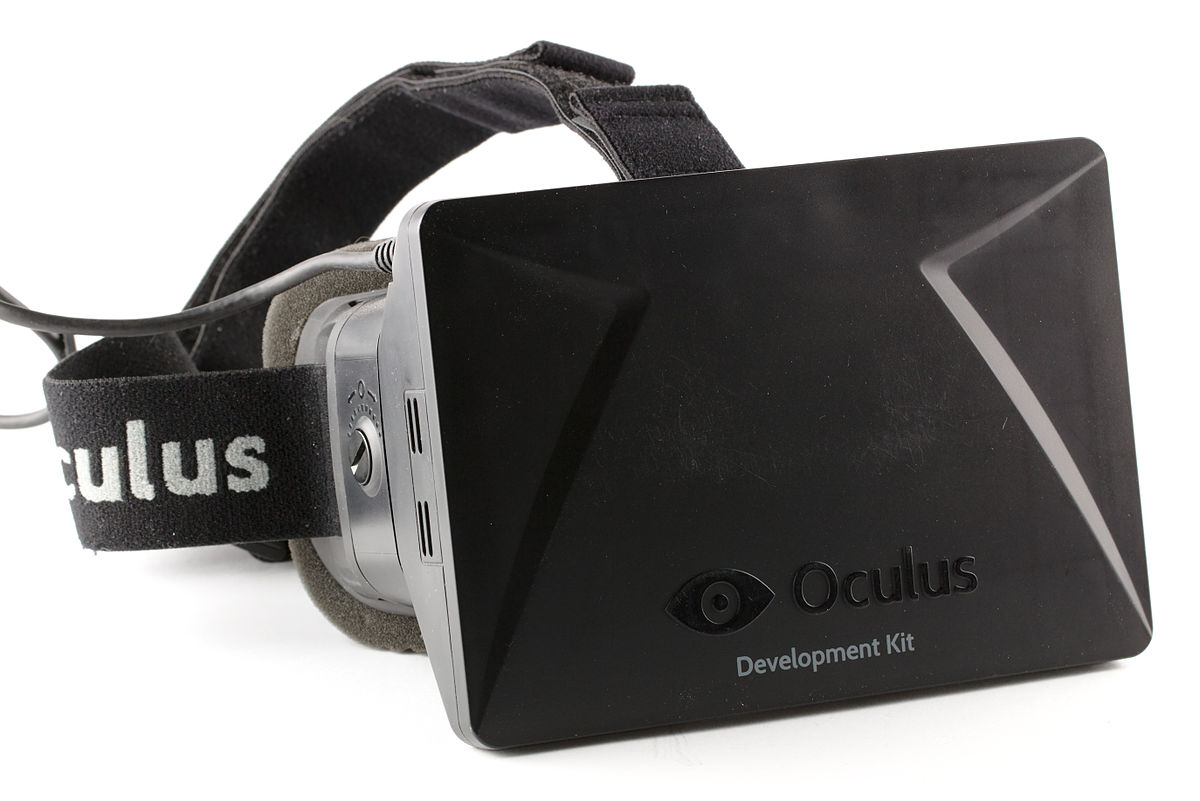
\includegraphics[width=3in]{proto_dk1.jpg}
    \caption{The original Oculus Rift Development Kit.}
    \label{fig:proto_oculus}
\end{figure}

\subsubsection{3D Printed Instruments}

A central tenant of our technical approach is to use physical, geometrically accurate instrument shapes that provide no functionality (i.e.\ no screens, no working buttons, etc.).
This is due to the motivation of being able to be used in an early design stage mockup.
In order to achieve this we have produced 3D-printed ``instruments'' that can be easily rearranged on a panel mount (pegboard).
Since the devices are rapidly prototyped, they can be redesigned in a much smaller time frame than typical simulator instruments.
By using the geometrically accurate instruments at the correct cockpit locations, the user is provided with accurate tactile and proprioceptive feedback without the need for entering the challenging field of virtual haptic feedback.

To use an instrument in the R3C system, it needs two versions of the 3D model.
The first is the version for the rendering engine, which requires textures and possible work to reduce the number of polygons so that rendering is not slowed down by the model.
The second model is for the 3D printing, which depending on the 3D printer used, will often require small changes to allow for a successful print.
Both of these require a surface mesh model.
Often, the original version exists as a CAD (Computer-Aided Design) model which typically does not describe the surface mesh directly but the geometric models that define the part.
The difficulty of the conversion from CAD to 3D model mesh can depend on the model, and the requirements of the rendering engine.

For this initial prototype, a demo instrument was developed based on a large multi-function display with edge keys.
The instrument model as viewed in the rendering engine is shown in Figure \ref{fig:proto_mfd_render}.
The 3D-printed version is shown pictured in Figure \ref{fig:proto_mfd_print}.
Notice that since it is only used for the tactile feel, it can have a plain aesthetic.
It was also printed in segments due to the limitations of the printer used.
The instrument mounted on a panel and being used is shown in Figure \ref{fig:proto_first_panel}.
This instrument provided a base for the demos, though it the specific design did not end up being used in a research study.
The workflow learned to create this demo instrument was also used for future instruments utilized in the research studies.

\begin{figure}
    \centering
    \begin{subfigure}[t]{0.32\linewidth}
        \centering
        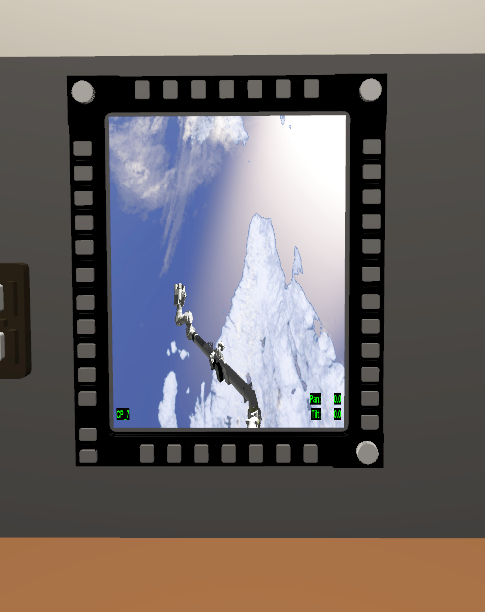
\includegraphics[width=\linewidth]{proto_mfd_render.jpg}
        \caption{The demo multifunction display instrument rendered in the virtual world.}
        \label{fig:proto_mfd_render}
    \end{subfigure}
    \begin{subfigure}[t]{0.32\linewidth}
        \centering
        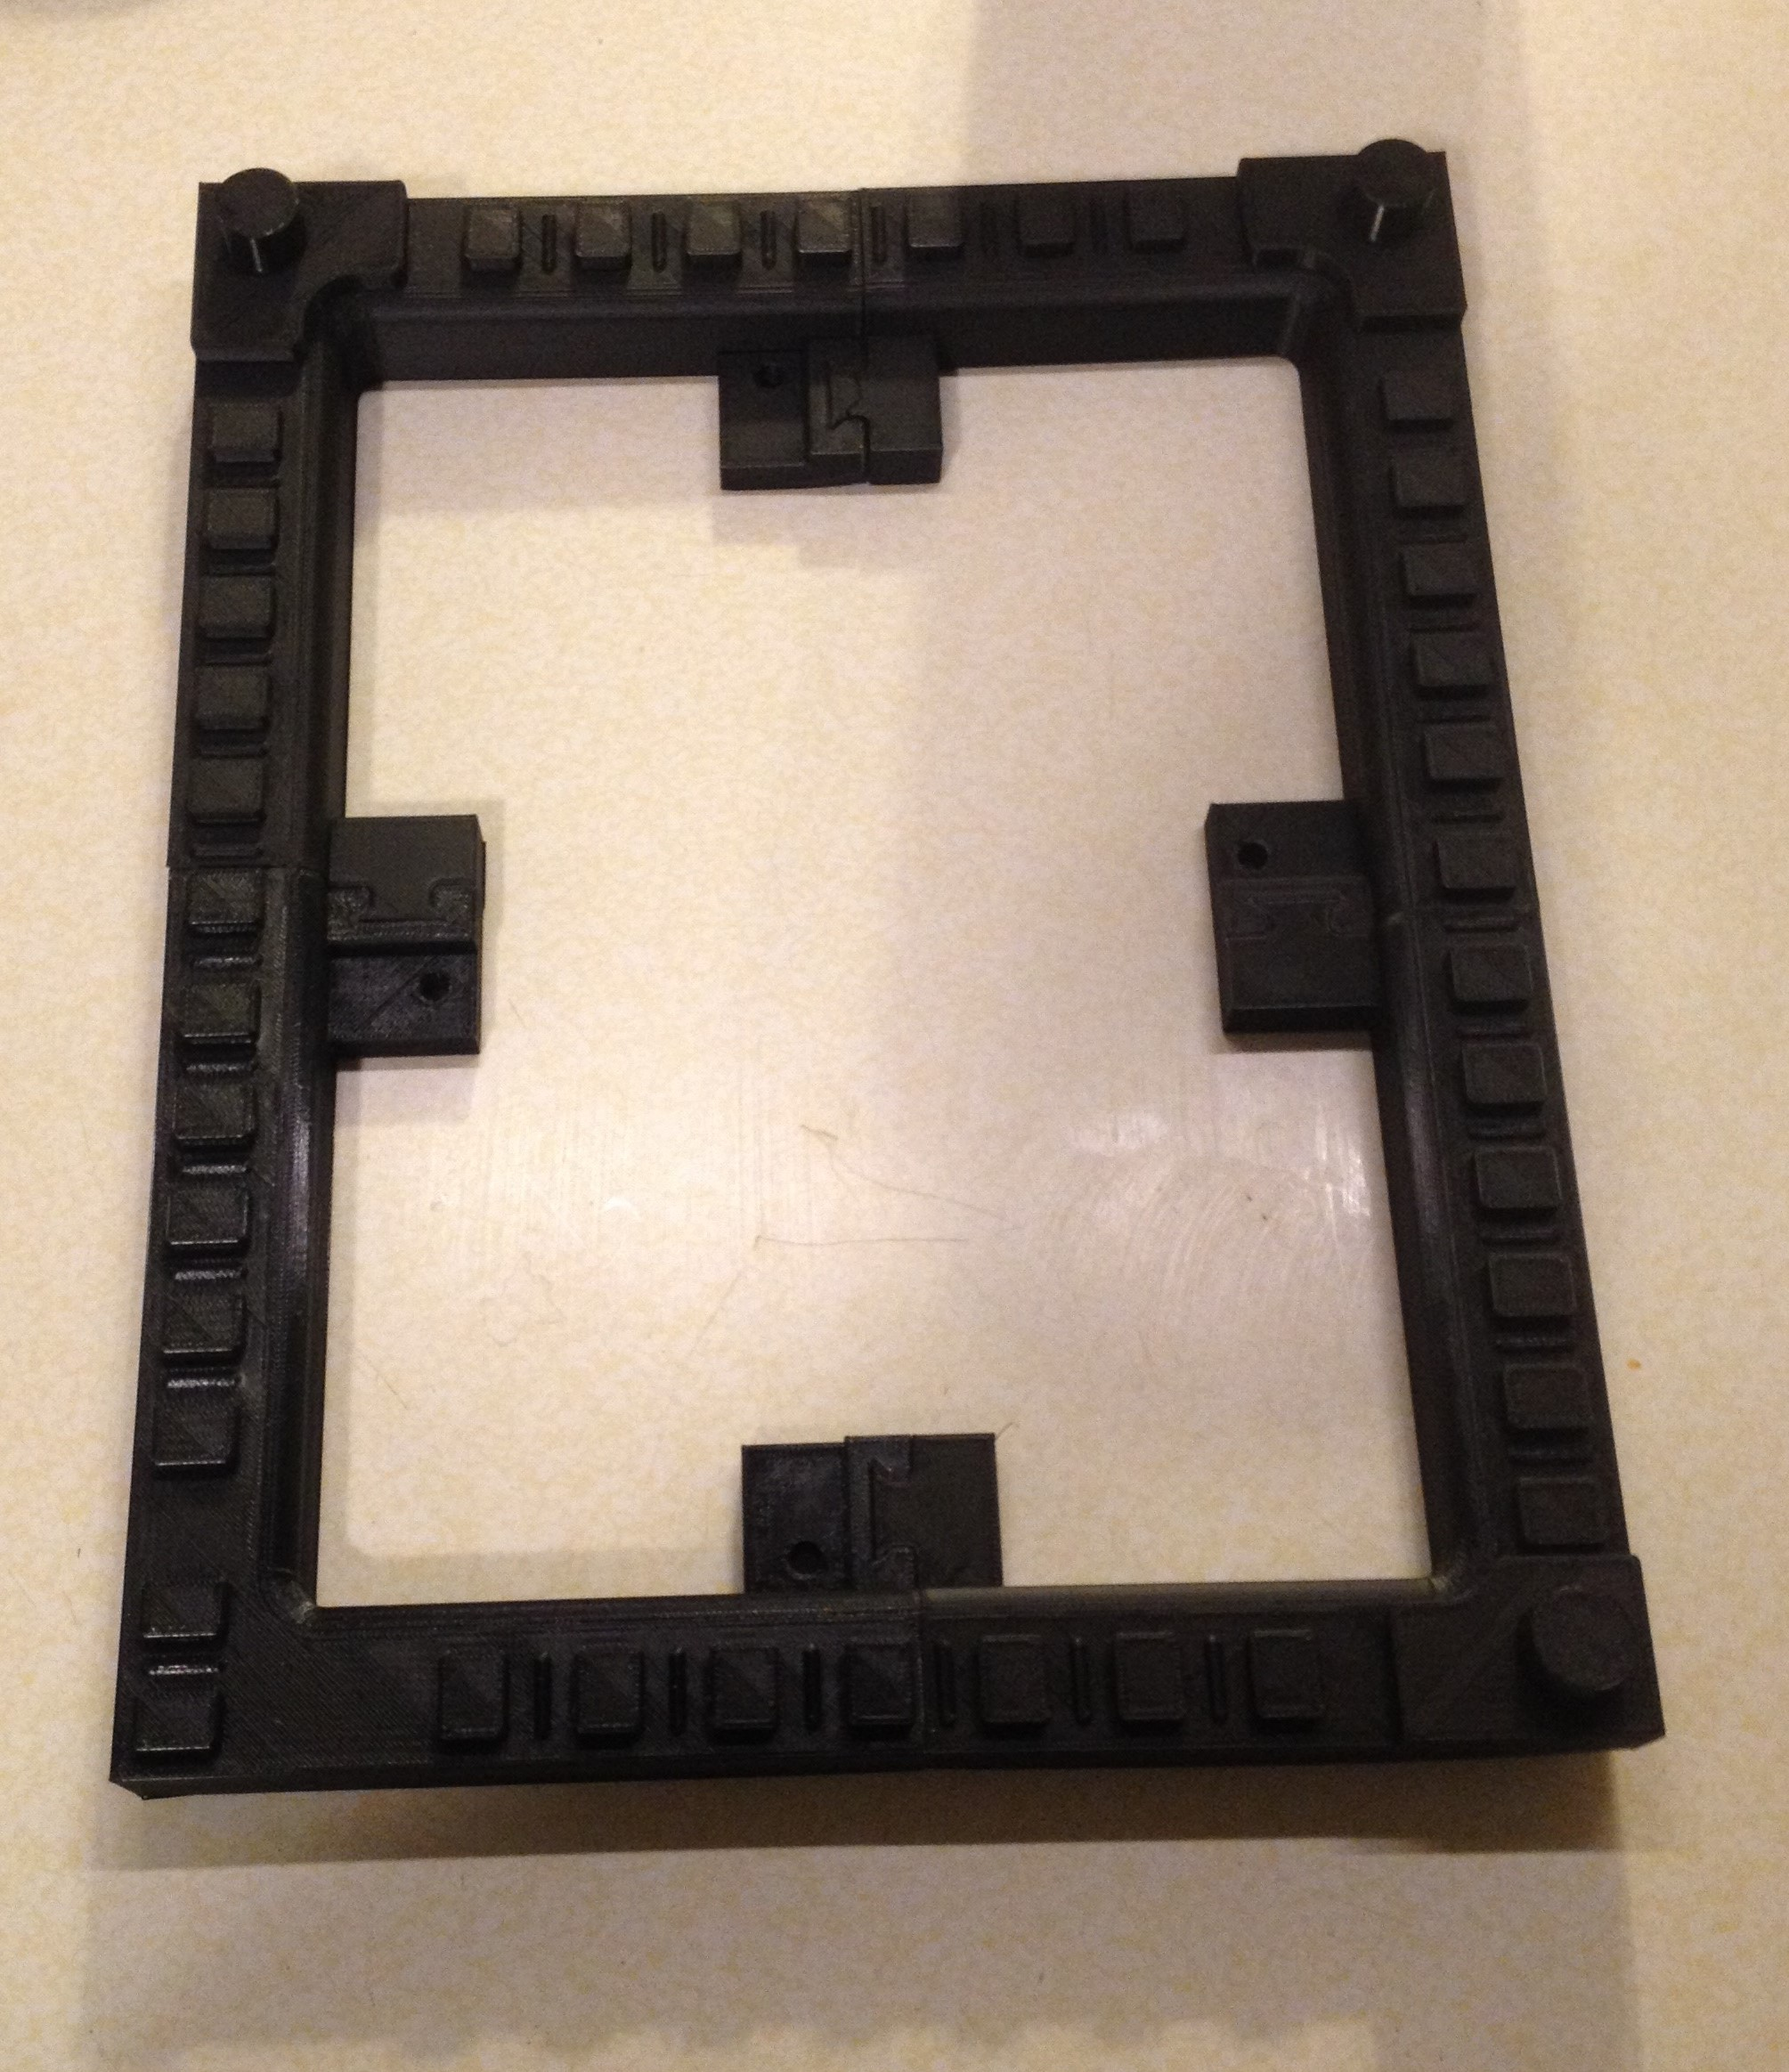
\includegraphics[width=\linewidth]{proto_mfd_print.jpg}
        \caption{The 3D printed version of the demo multifunction display instrument.}
        \label{fig:proto_mfd_print}
    \end{subfigure}
    \begin{subfigure}[t]{0.32\linewidth}
        \centering
        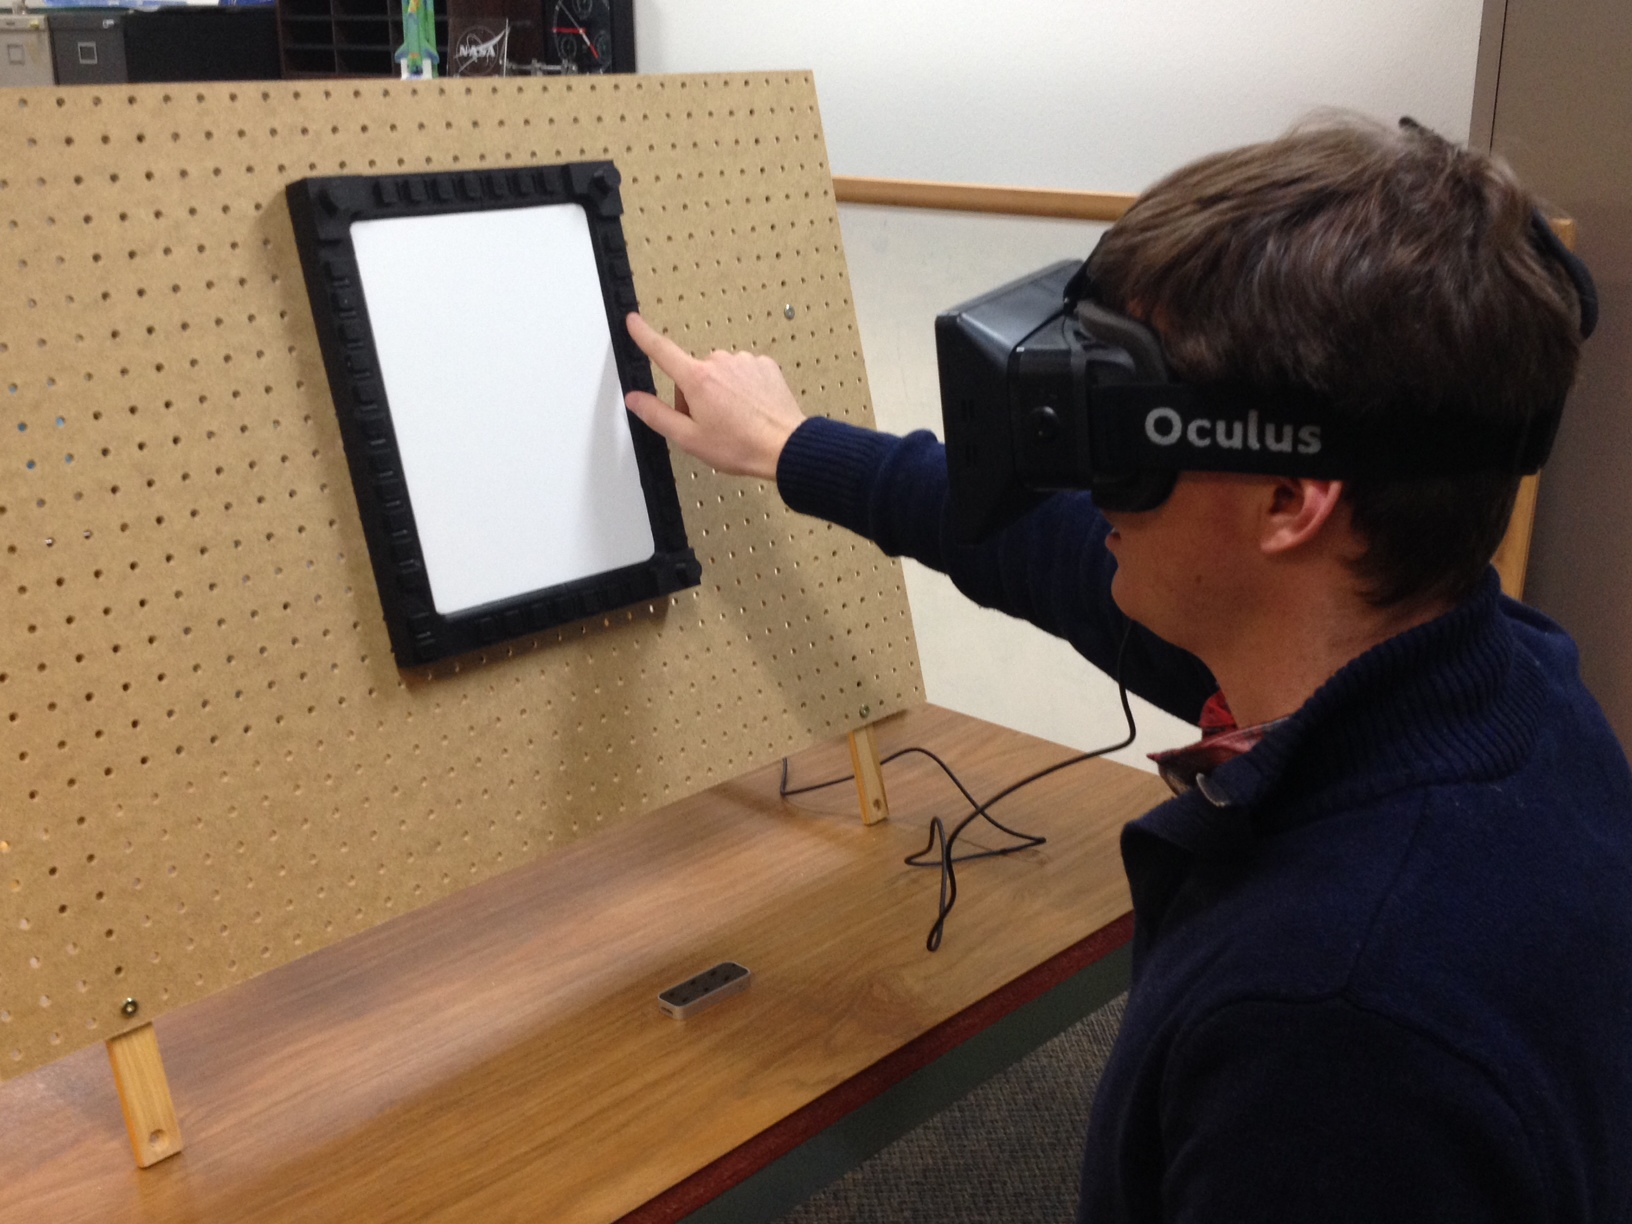
\includegraphics[width=\linewidth]{proto_first_panel.jpg}
        \caption{The demo multifunction display instrument mounted on a panel.}
        \label{fig:proto_first_panel}
    \end{subfigure}
\end{figure}


\subsubsection{Hand Tracking}

The LeapMotion hand tracker was selected as it provided an unobtrusive method for hand tracking.
The device itself is small (3 in x 1.2 in x 0.5 in), allowing it to be used in constrained environments (pictured in Figure \ref{fig:proto_leap_device}).
It uses two infrared cameras as the source of its proprietary tracking algorithm, and requires no gloves to be worn by the user.
The tracking volume extends about 2 feet above the controller, and about 2 feet about the center on the other two axes.
This large field of view is shown in Figure \ref{fig:proto_leap_fov} and can easily cover the working area of a cockpit panel.
The original version of the software, used in this prototype, provided information on the location and orientation of each fingertip.
It also gave the position and orientation of the palm, but did not provide any details on the joints or which finger of the hand the fingertip belonged to.
The tracking rate is approximately 120Hz, with an advertised latency of milliseconds.

\begin{figure}
    \centering
    \begin{subfigure}[t]{0.49\linewidth}
        \centering
        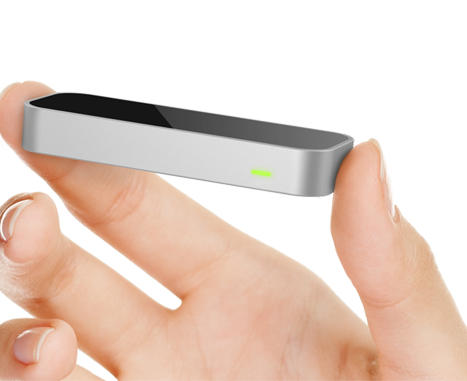
\includegraphics[width=\linewidth]{leapmotion.png}
        \caption{LeapMotion device.}
        \label{fig:proto_leap_device}
    \end{subfigure}
    \begin{subfigure}[t]{0.49\linewidth}
        \centering
        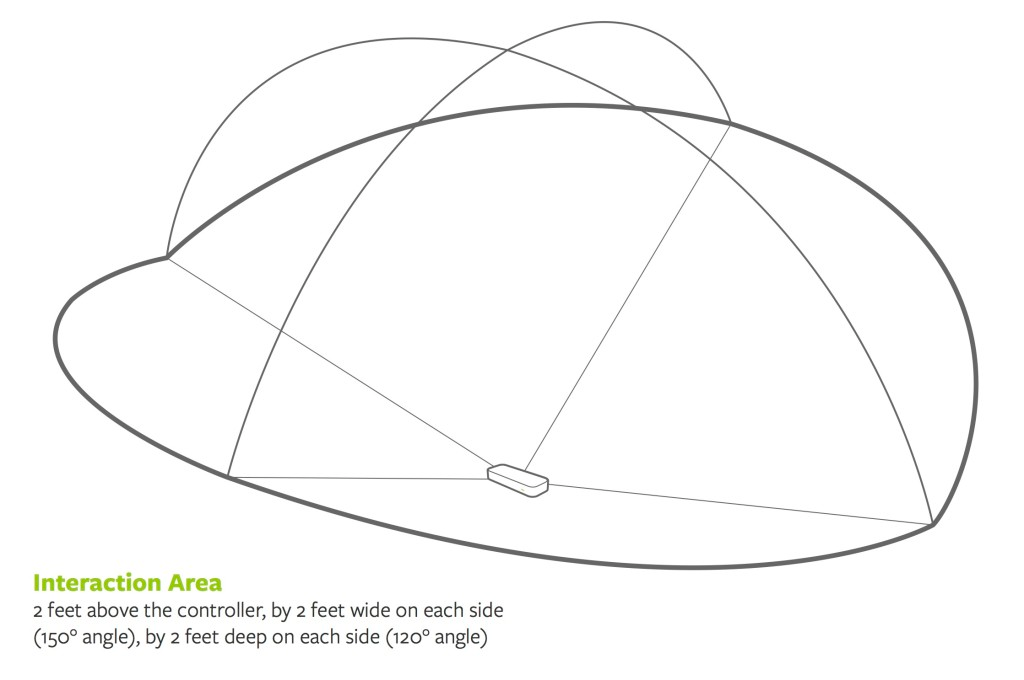
\includegraphics[width=\linewidth]{leapmotion_fov.png}
        \caption{LeapMotion field of view.}
        \label{fig:proto_leap_fov}
    \end{subfigure}
    \caption{The LeapMotion device and field of view. Images by LeapMotion.}
    \label{fig:proto_leap}
\end{figure}

\subsubsection{Button Input Recognition}
\label{sec:proto_button_input}

As part of the motivation and requirements of our approach, the hand tracker data needs to be used to determine when a user is pushing a button.
The goal is to be able to use this system on top of a non-functioning mockup, thus all interactivity must be performed with the hand tracker.
With a working hand tracking system, the next step was to develop a method to determine when users were pushing a button.
The button recognition system was developed within the EDGE engine independent to the hand tracker, so that future prototypes could use a different hand tracker if a new device were released.

The button detection algorithm is a simple collision detection model.
A rectangular box is defined that extends outside the button, including a tolerance zone to account for misalignment and poor tracking.
When a fingertip enters and stays in the box for approximately 150ms\footnote{This time is configurable and was often tweaked for each experiment.} then a button event is triggered.
The purpose of the delay is to account for false positives when a user might accidentally enter the box without intention to press the button.
The advantage to using the optical tracking to determine when a user has selected a button is that it has the potential to significantly reduce the complexity of the system.
If the user interactions with the panel can be determined solely by tracking his/her hands from the external sensor, then the cockpit panel needs only to provide physical feedback, and does not require any wiring.

\subsubsection{Challenges}

The hand tracking caused two issues with the use of the prototype.
The first was simply that the reliability of the tracking caused many instances of dropped tracking, causing fingers to disappear unexpectedly.
The second was the conversion between hand tracker coordinates and instrument coordinates.
The registration between the virtual and physical worlds was difficult to get right with this configuration.
Even with precise alignment of the hand tracker, the fingertip positions did not always align properly with the buttons in the virtual world when a subject had their finger on and felt a physical button.
Since the hand tracking was not very reliable, many users would almost completely ignore its input and find the buttons by proprioception and tactile feedback.
This then led to confusion as the button would not register a button press but the strong tactile feedback meant they would not leave the physical button to hunt for the virtual button location.

Another challenging portion of the registration was that since the Oculus Rift did not have head positioning, the head position would have to be set manually.
Depending on the actual position of the user, the panel would not appear with the correct scale and at the correct distance in the virtual world.
This caused users to initially reach too short or too far for the panel, or decreased the realism as the panel seemed too small or large compared to the real world object.
Since the head tracking sensors were all internal to the headset, it also experienced drift after a few minutes.
Most noticeable in the yaw, it would cause the panel to become misaligned and require a manual reset to realign.

\subsection{Second Prototype}

A number of improvements were made in the second generation of the prototype.
Due to software upgrades, the hand tracking became more robust and provided more complete information about the entire hand position.
The visuals were upgraded to the second Development Kit of the Oculus Rift, which provided improved visual resolution but more importantly an external head tracker (camera) which enabled head movement and virtually eliminated drift of the internal sensors.
A major focus of this version of the development work for this prototype was to improve reliability and registration.
The reliability was partially improved with the new hand tracking software, but other countermeasures developed are described as well.
Registration, which refers to the alignment between the physical world and the virtual world, was improved with the use of a new calibration mechanism described in this section.

\begin{figure}
    \centering
    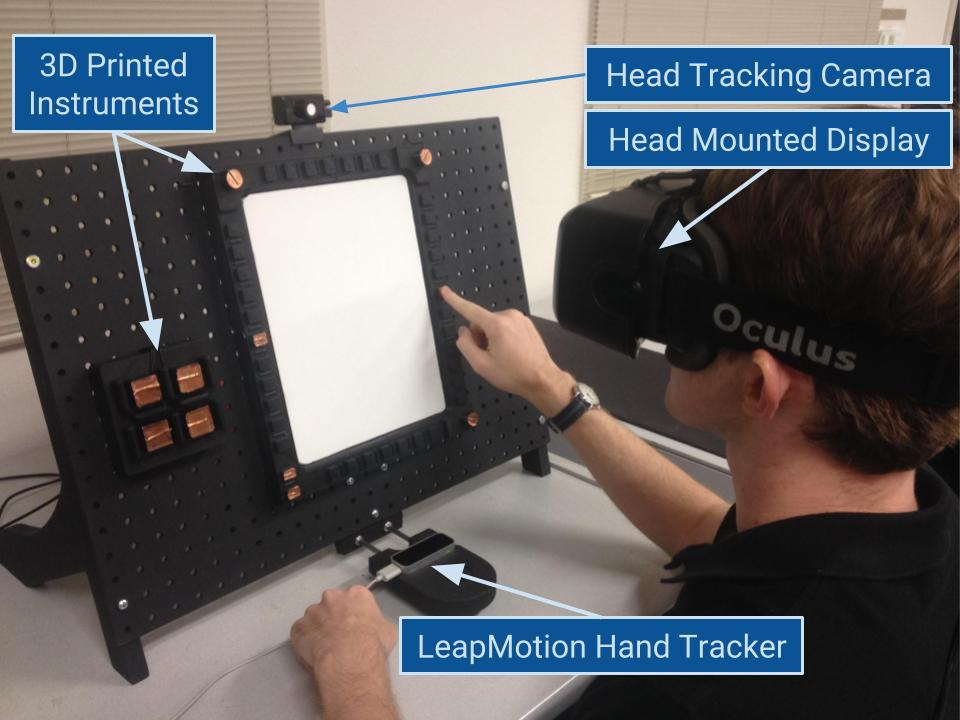
\includegraphics[width=\linewidth]{r3c_callout.jpg}
    \caption{A version of the second prototype with major components noted.}
    \label{fig:r3c_callout}
\end{figure}

\subsubsection{Virtual Reality Headset}

The head tracking provided in the newest development kit version gives a significant improvement over the original Oculus Rift in the registration between the real world and the virtual world.
This allowed the user to lean and gain additional perspective on the virtual world that was not possible with the first version.
The position and orientation is reported relative to the tracking camera which is placed facing the user.
For our application, with a well known location of the camera relative to the panel, the head position can be placed in the virtual world at the exact location of the user's actual head position.
Unlike with the first version, the virtual components are now always rendered at the correct distance and with proper scale.
The head-tracking camera is shown mounted on the instrument panel in Figure \ref{fig:r3c_callout}.


\subsubsection{Hand Tracking}

The upgrade to the hand tracking software provided two features that were integrated.
The first was an improvement in the fidelity of the tracking, including full information on the joints of the hand.
The second was the introduction of a ``head mounted'' mode, which allowed for tracking to be optimized for looking down at a hand.

The tracking upgrade adds the location and orientation of the entire hand at a skeletal level.
This means all the joints are tracked and the bones between them.
The upgraded view is shown in Figure \ref{fig:proto_skeleton}.
This provided a more immersive feeling than the floating fingers of the original prototype.

\begin{figure}
    \centering
    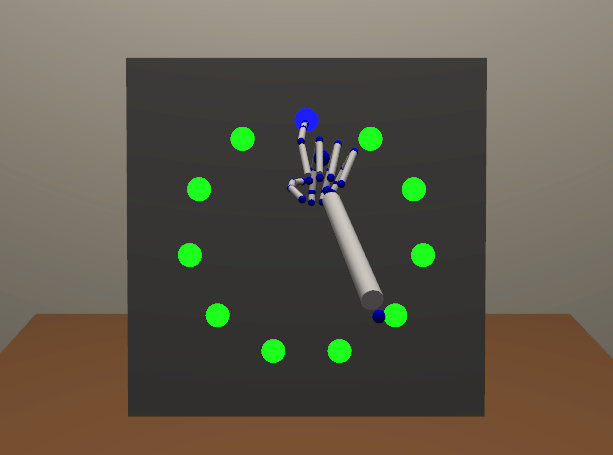
\includegraphics[width=\linewidth]{leap_skeleton.png}
    \caption{The complete hand tracking of the LeapMotion v2 software.}
    \label{fig:proto_skeleton}
\end{figure}

At the same time of the tracking upgrade, a ``VR Mode'' was introduced to the LeapMotion software to provide hand tracking in a virtual environment by way of mounting it on the head-mounted display itself.
Upon initial testing of this feature, two observations were made.
The tracking was much improved when the tracker was looking down at the hands, seemingly providing more robust and reliable tracking data.
However, using it mounted to the head-mounted display caused a larger disconnect between the real world and physical world.
The registration between the hand tracker and the location of the instruments relies on a known, rigid connection.
When the tracker was mounted on the head-mounted display, the transformation between LeapMotion coordinates and panel coordinates relied on knowing the location of the head.
Although this information could be obtained from the newer model HMD which included head tracking, it was simply not precise or stable enough to use as the base for the hand tracking coordinates.
For example, if a hand was placed resting on the panel and kept still, the virtual hand would appear to move relative to the virtual panel if the head were moved at even a moderate pace.
The additional latency introduced by relying on the head tracking sensors simply would not keep accurate registration.
This led us to develop a mount that would hold the LeapMotion upside down over the panel and instruments (Figure \ref{fig:proto_leap_mount}).
The software could still be configured to the ``VR Mode'', optimizing for face-down tracking, but with a rigid mount.
This provided the best of both worlds: reliability of the face-down tracking with a stable transformation between the tracker coordinates and the panel coordinates.

\begin{figure}
    \centering
    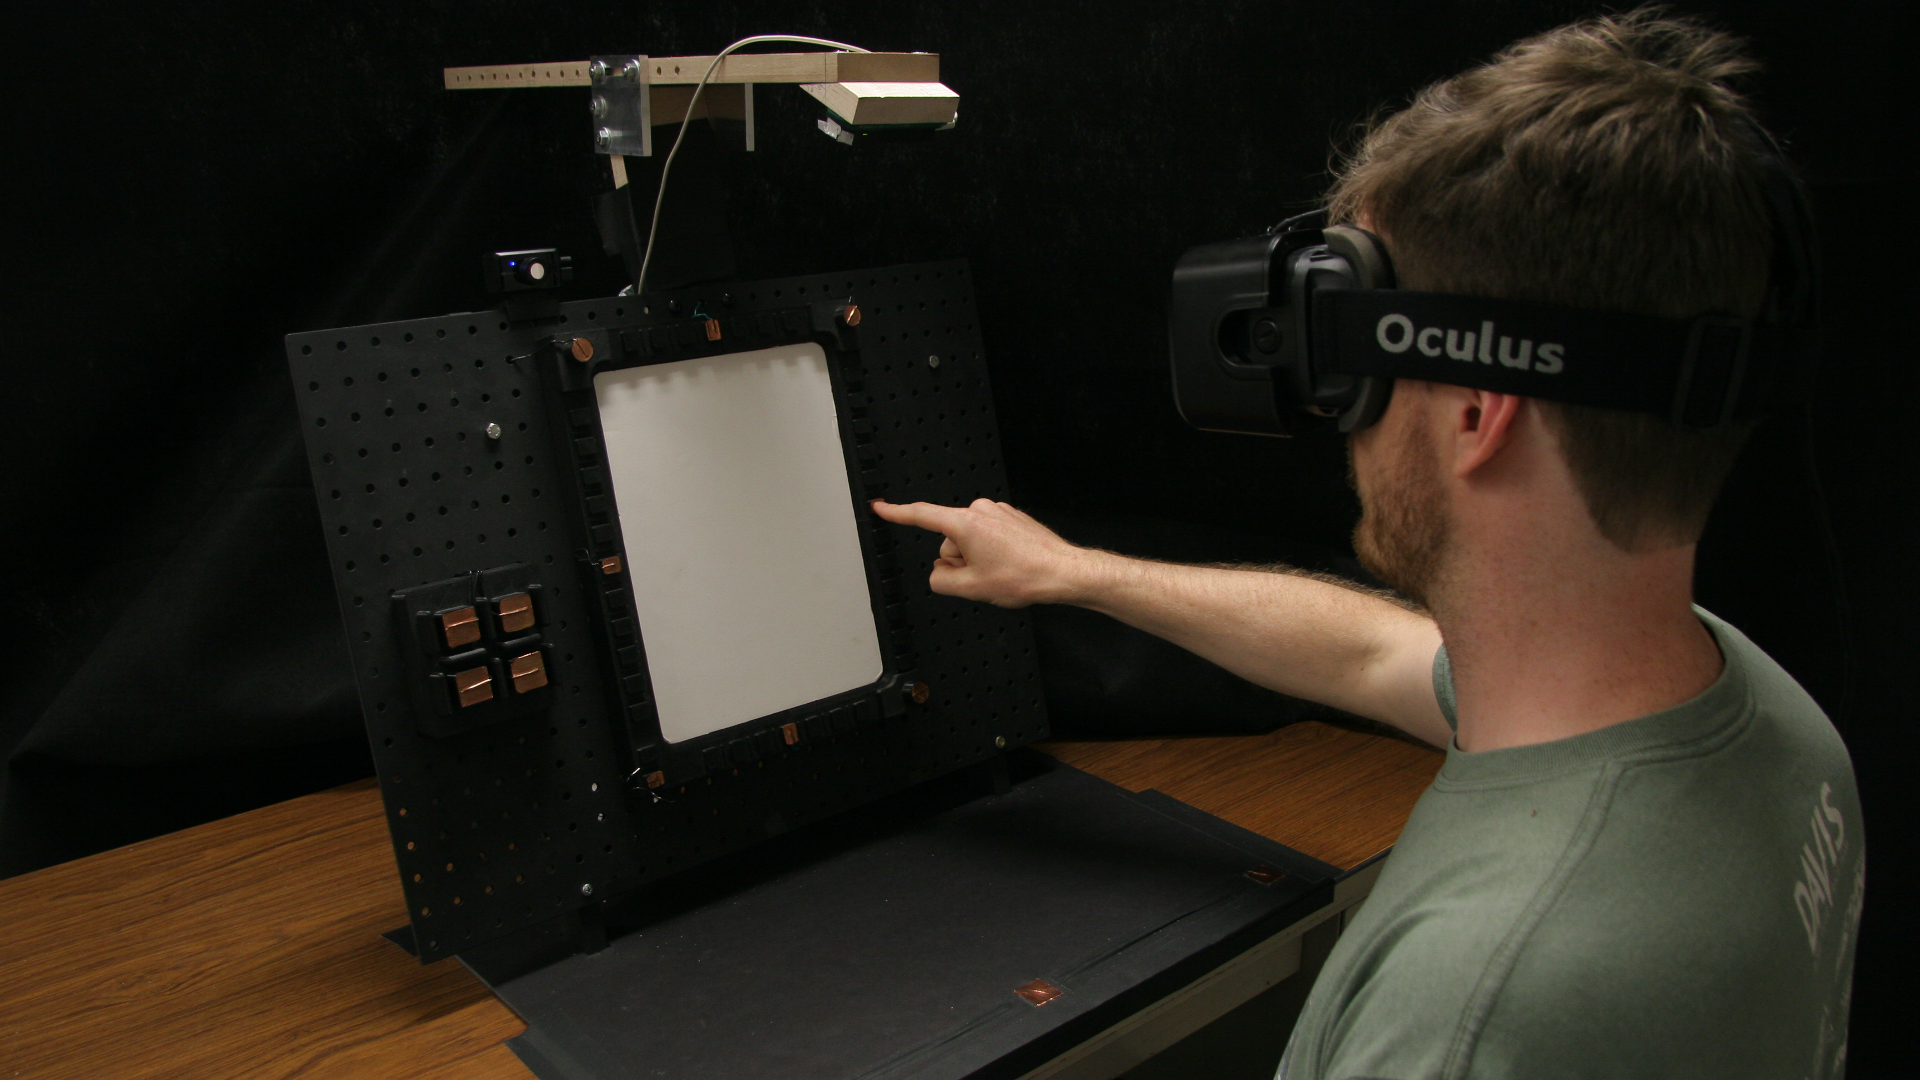
\includegraphics[width=\linewidth]{leap_mount.jpg}
    \caption{The LeapMotion mount, holding the sensor above the panel and looking down.}
    \label{fig:proto_leap_mount}
\end{figure}

\subsubsection{Button Recognition Countermeasures}

%onboarding
Two countermeasures were introduced in this prototype that aided new users in learning the button recognition algorithms of the hand tracker.
A simple visual indication was added when a user entered the zone in front of the button.
This was typically implemented with the button itself being highlighted or changing color.
With this crucial feedback, new users were able to learn the tolerances of the button zone and understand when the button was going to be `pressed'.
For experienced users, the feedback provided confirmation that they were in the zone and were not waiting for it to register incorrectly.
The second countermeasure was the addition of an aural feedback upon the button press being registered.
A simple ``click'' noise was played when the button press event occurred, confirming the button press to the user on a quicker cognitive channel than processing if the expected change on the instrument occurred.
At the same time, the button highlight was restored to the original non-highlighted state, providing feedback in both visual and aural channels.
These countermeasures were observed as being very helpful to new users, and were included in all of the research studies.

\subsubsection{Capacitive Touch Sensors}
\label{sec:proto_cap_touch}

In order to be able to activate the buttons reliably when the hand tracking was degraded or dropped out, it was decided to investigate the use of capacitive touch sensors.
The capacitive touch sensors were initially developed as a countermeasure to the problems encountered with the hand tracking from the original prototype.
As the hand tracking became more robust with the new software from the manufacturer, the countermeasure was not as important, but the sensors played a new role in the prototype: validating the accuracy, and providing calibration for the hand tracker.

With the goal of minimal setup, the original capacitive touch sensors were developed with copper tape electrodes placed on the top of the 3D printed instrument buttons.
These electrodes are shown on the demo multifunction instrument in Figure \ref{fig:copper_pads}.
A Freescale MPR121 capacitive touch sensor was used to read the electrodes and communicate with an Arduino which sent touch events over a serial communication line to the computer.
These serial events were read by the rendering engine to trigger events when a copper pad was touched.
These simple, single electrode per button sensors provided a reliable method for determining when the user had actually touched a button.
The main use of these sensors evolved to be for the calibration mechanism described in the next section.
However, as the registration improved, a research question was developed around how accurate the user could be on the physical device while immersed visually in the virtual world.
This led to the development of a second generation of capacitive touch buttons, used in the Pointing Experiment (Chapter \ref{chap:pointing}).

\begin{figure}
    \centering
    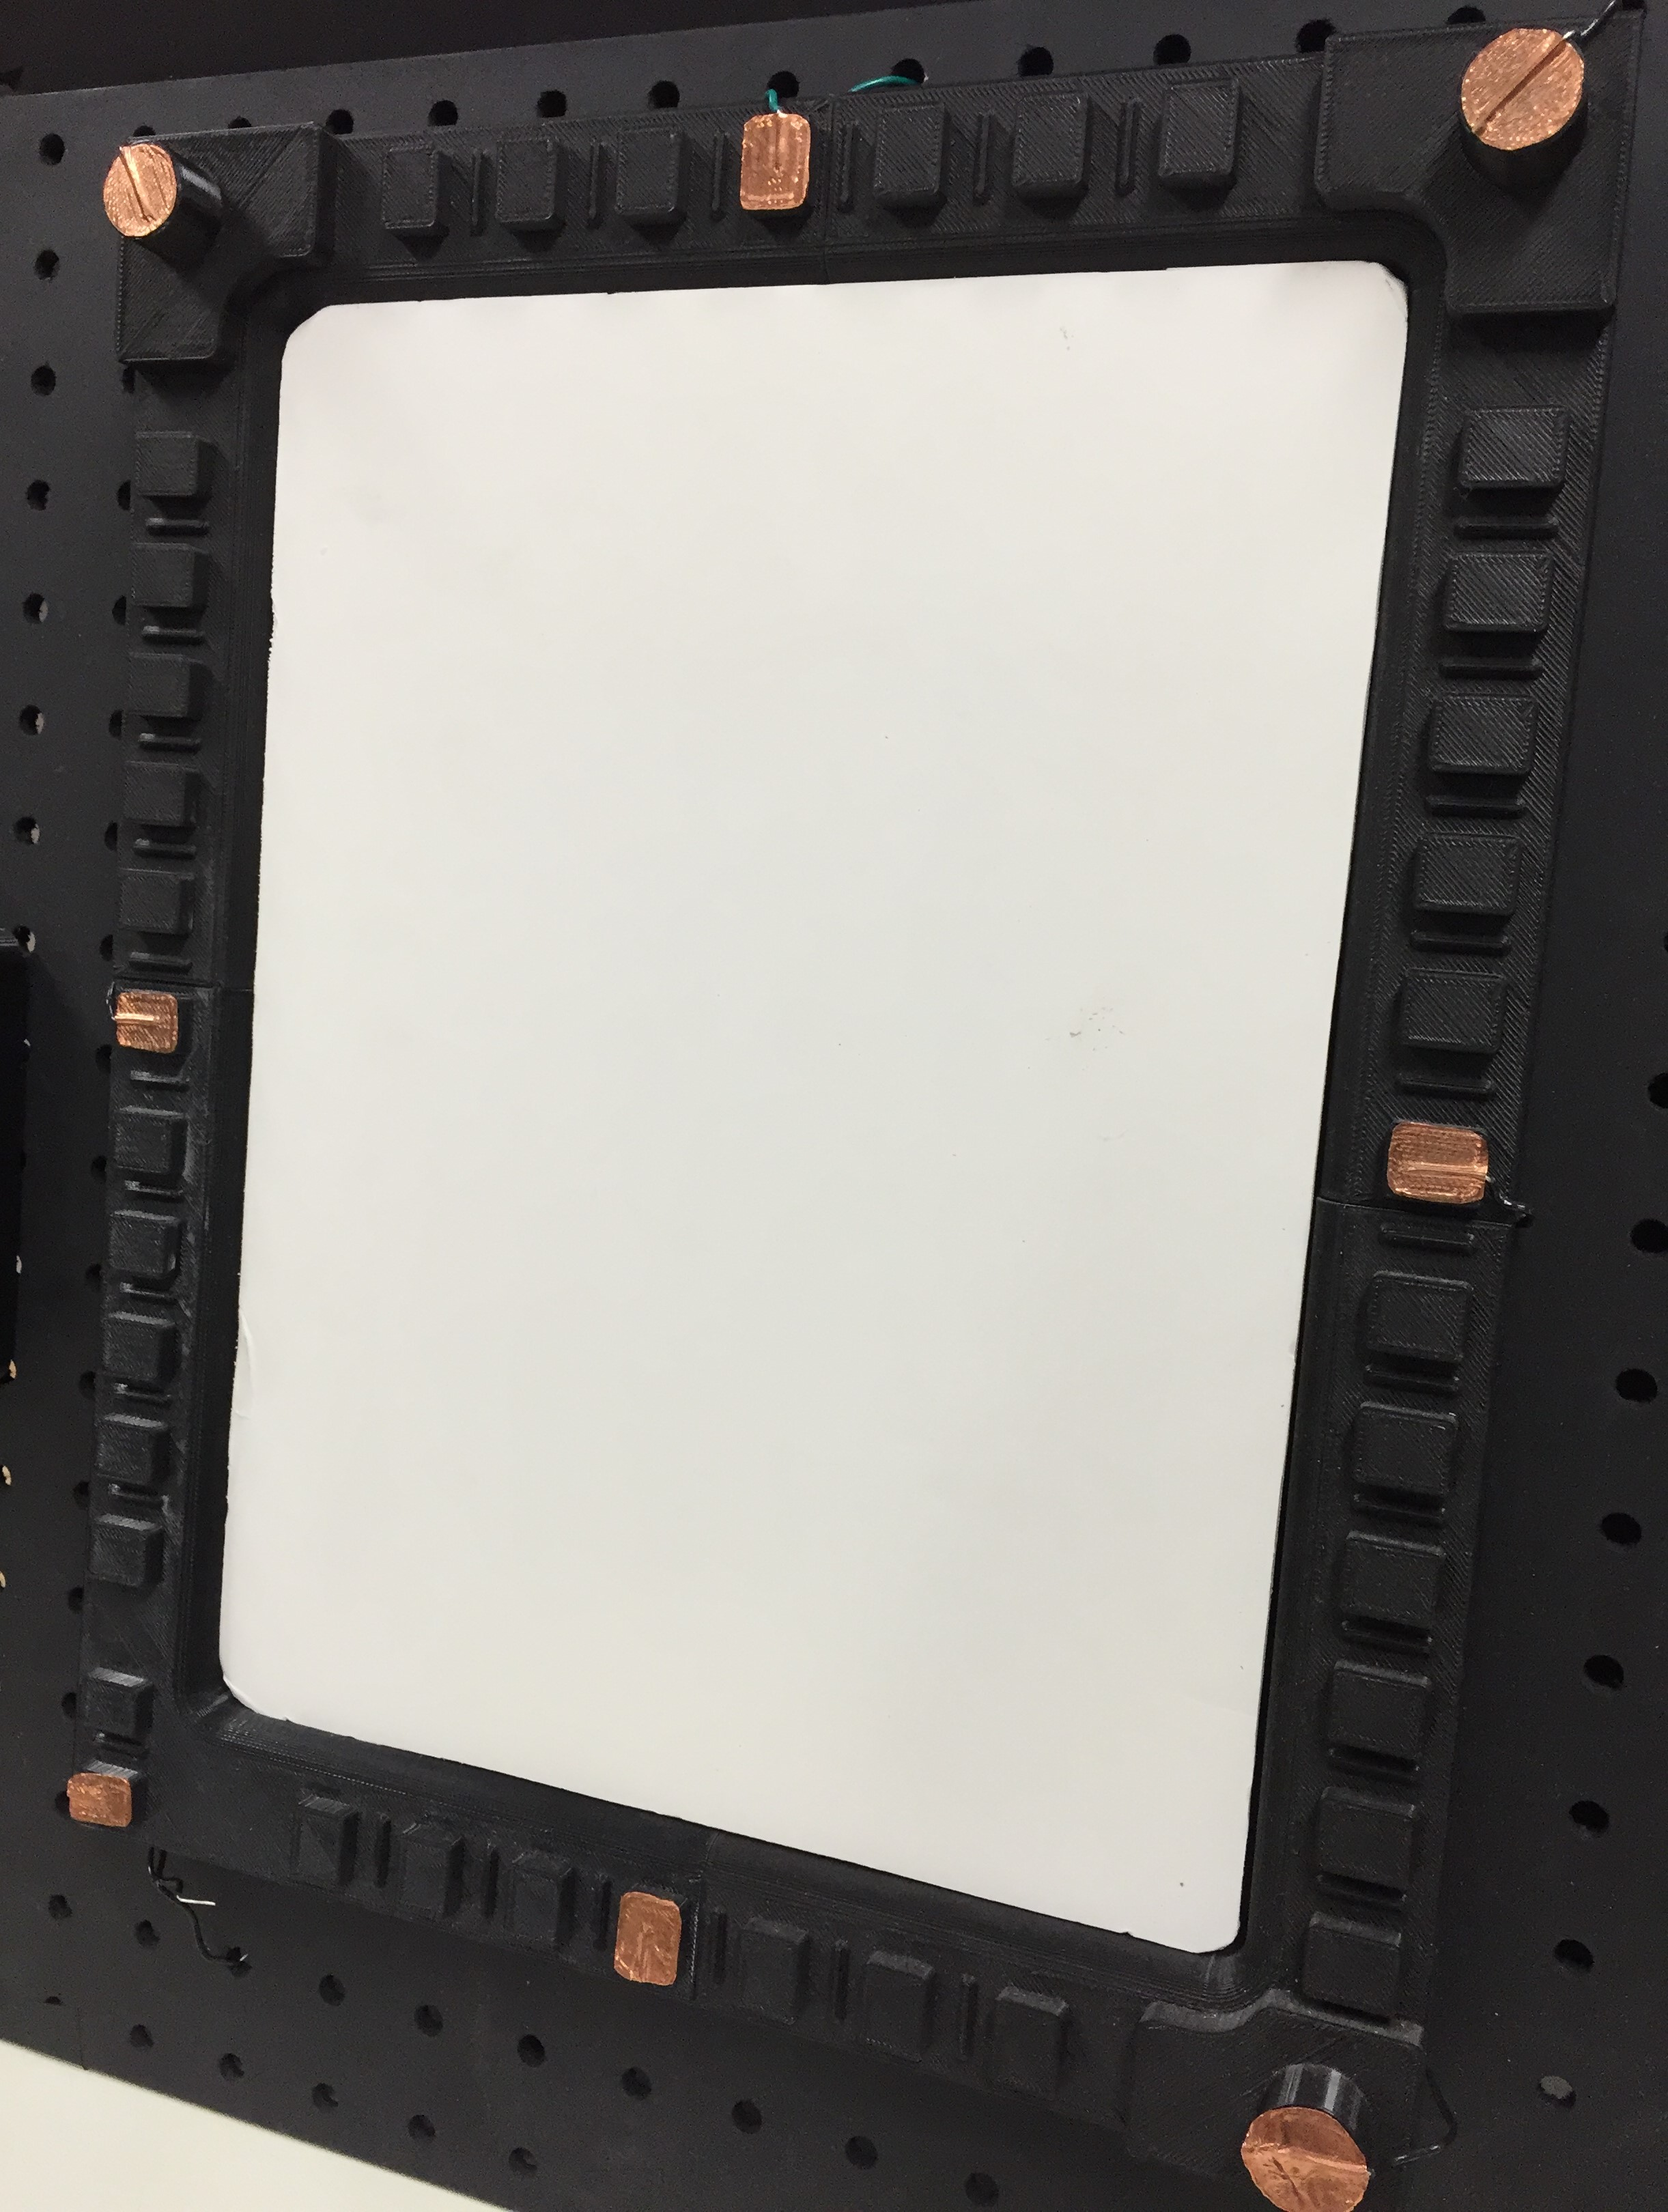
\includegraphics[width=0.5\linewidth]{copper_pads.jpg}
    \caption{The copper tape electrodes for capacitive touch sensings on the demo multifunction instrument.}
    \label{fig:copper_pads}
\end{figure}

Since touch accuracy can be important in safety-critical applications, we developed the ability to record where on the button the finger press was located using a capacitive touch sensor.
To accomplish this, a custom printed circuit board was developed that provides an electrode array of 5 rows and 5 columns over a 1-inch by 1-inch square.
This board is show in Figure \ref{fig:proto_capacitive_array}.%, where it is mounted in a 3D printed instrument.
The capacitive state of each row and column can provide a measurement of the center of the finger press on the grid created by the rows and columns.
Finger location accuracy of under 0.1-inch can be achieved with this configuration.
The location of the finger press can help provide a measure of the accuracy of the registration between the optical sensors and the real world location, as well as any bias introduced from using the VR headset and hand tracker.

\begin{figure}
    \begin{subfigure}[t]{0.32\linewidth}
    \centering
    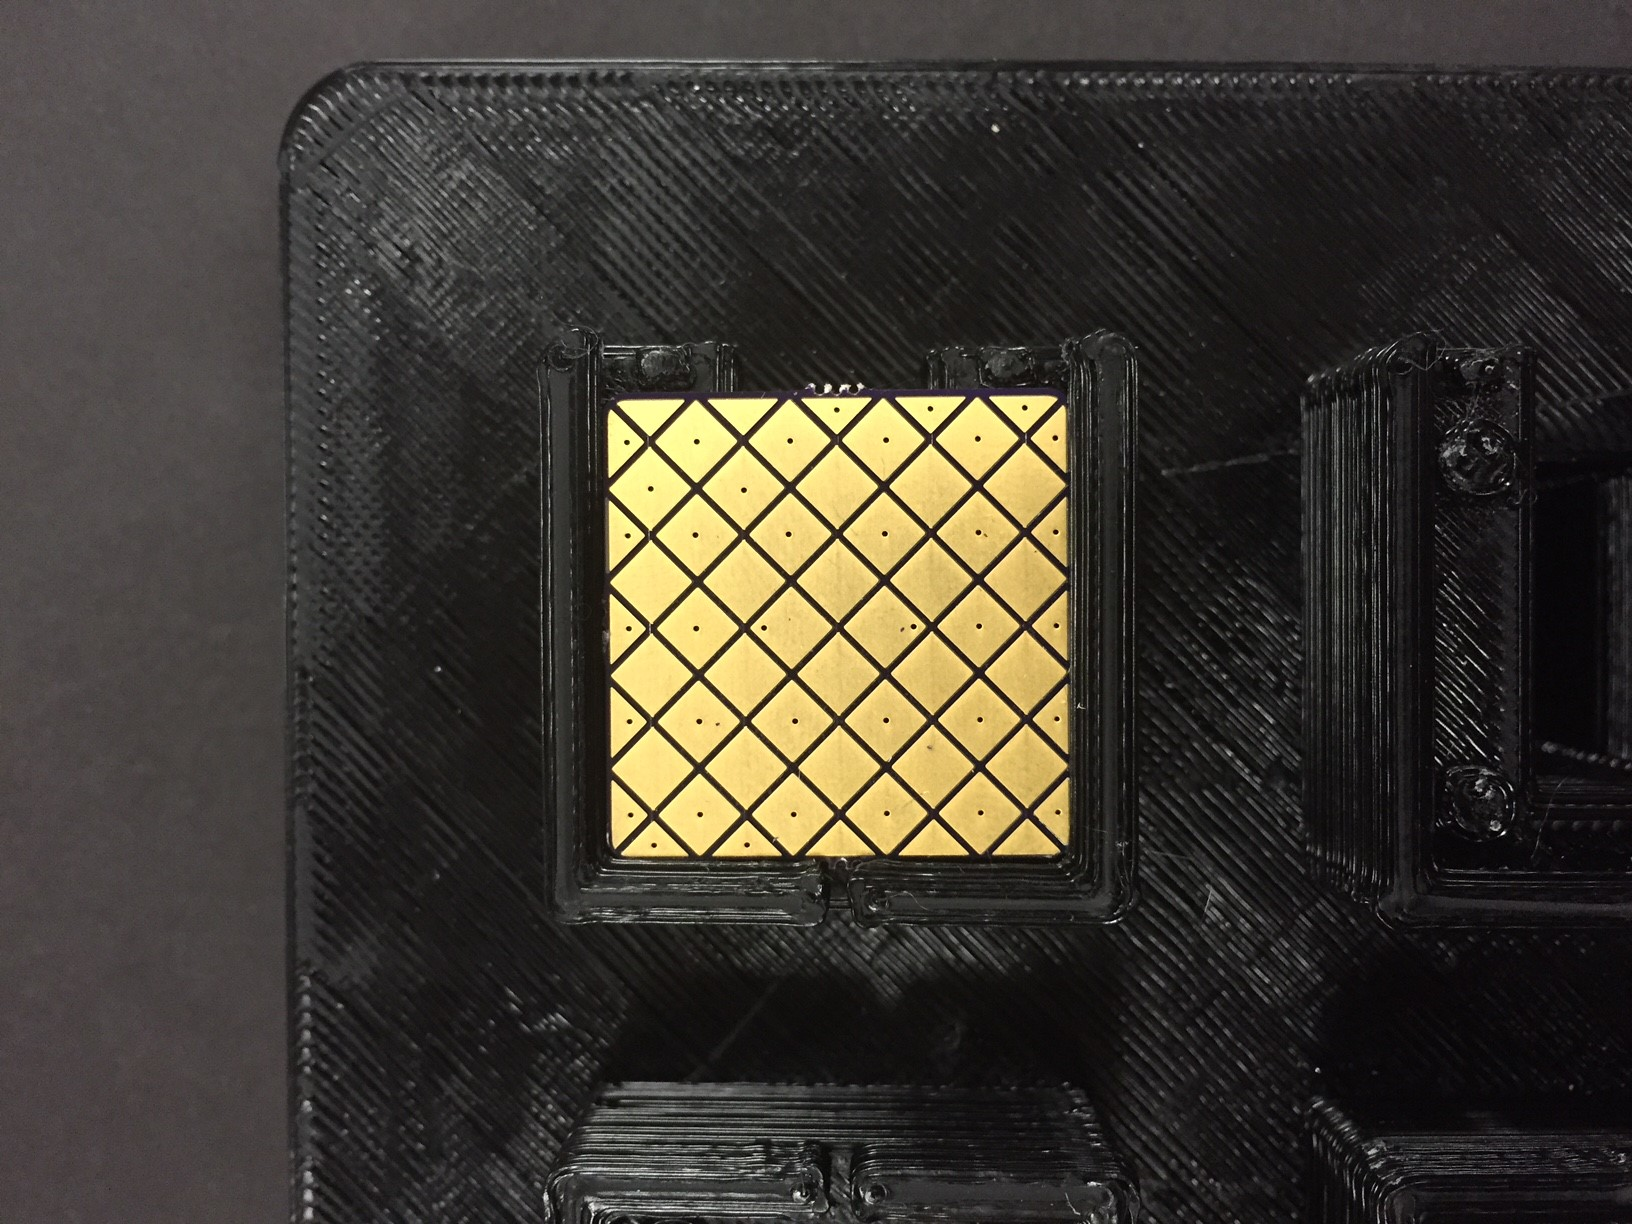
\includegraphics[width=1.5in]{pe_capacitive.jpg}
    \caption{Capactive array mounted in a 3D printed button.}
    \label{fig:proto_capacitive_array:mounted}
    \end{subfigure}
    \begin{subfigure}[t]{0.64\linewidth}
    \centering
        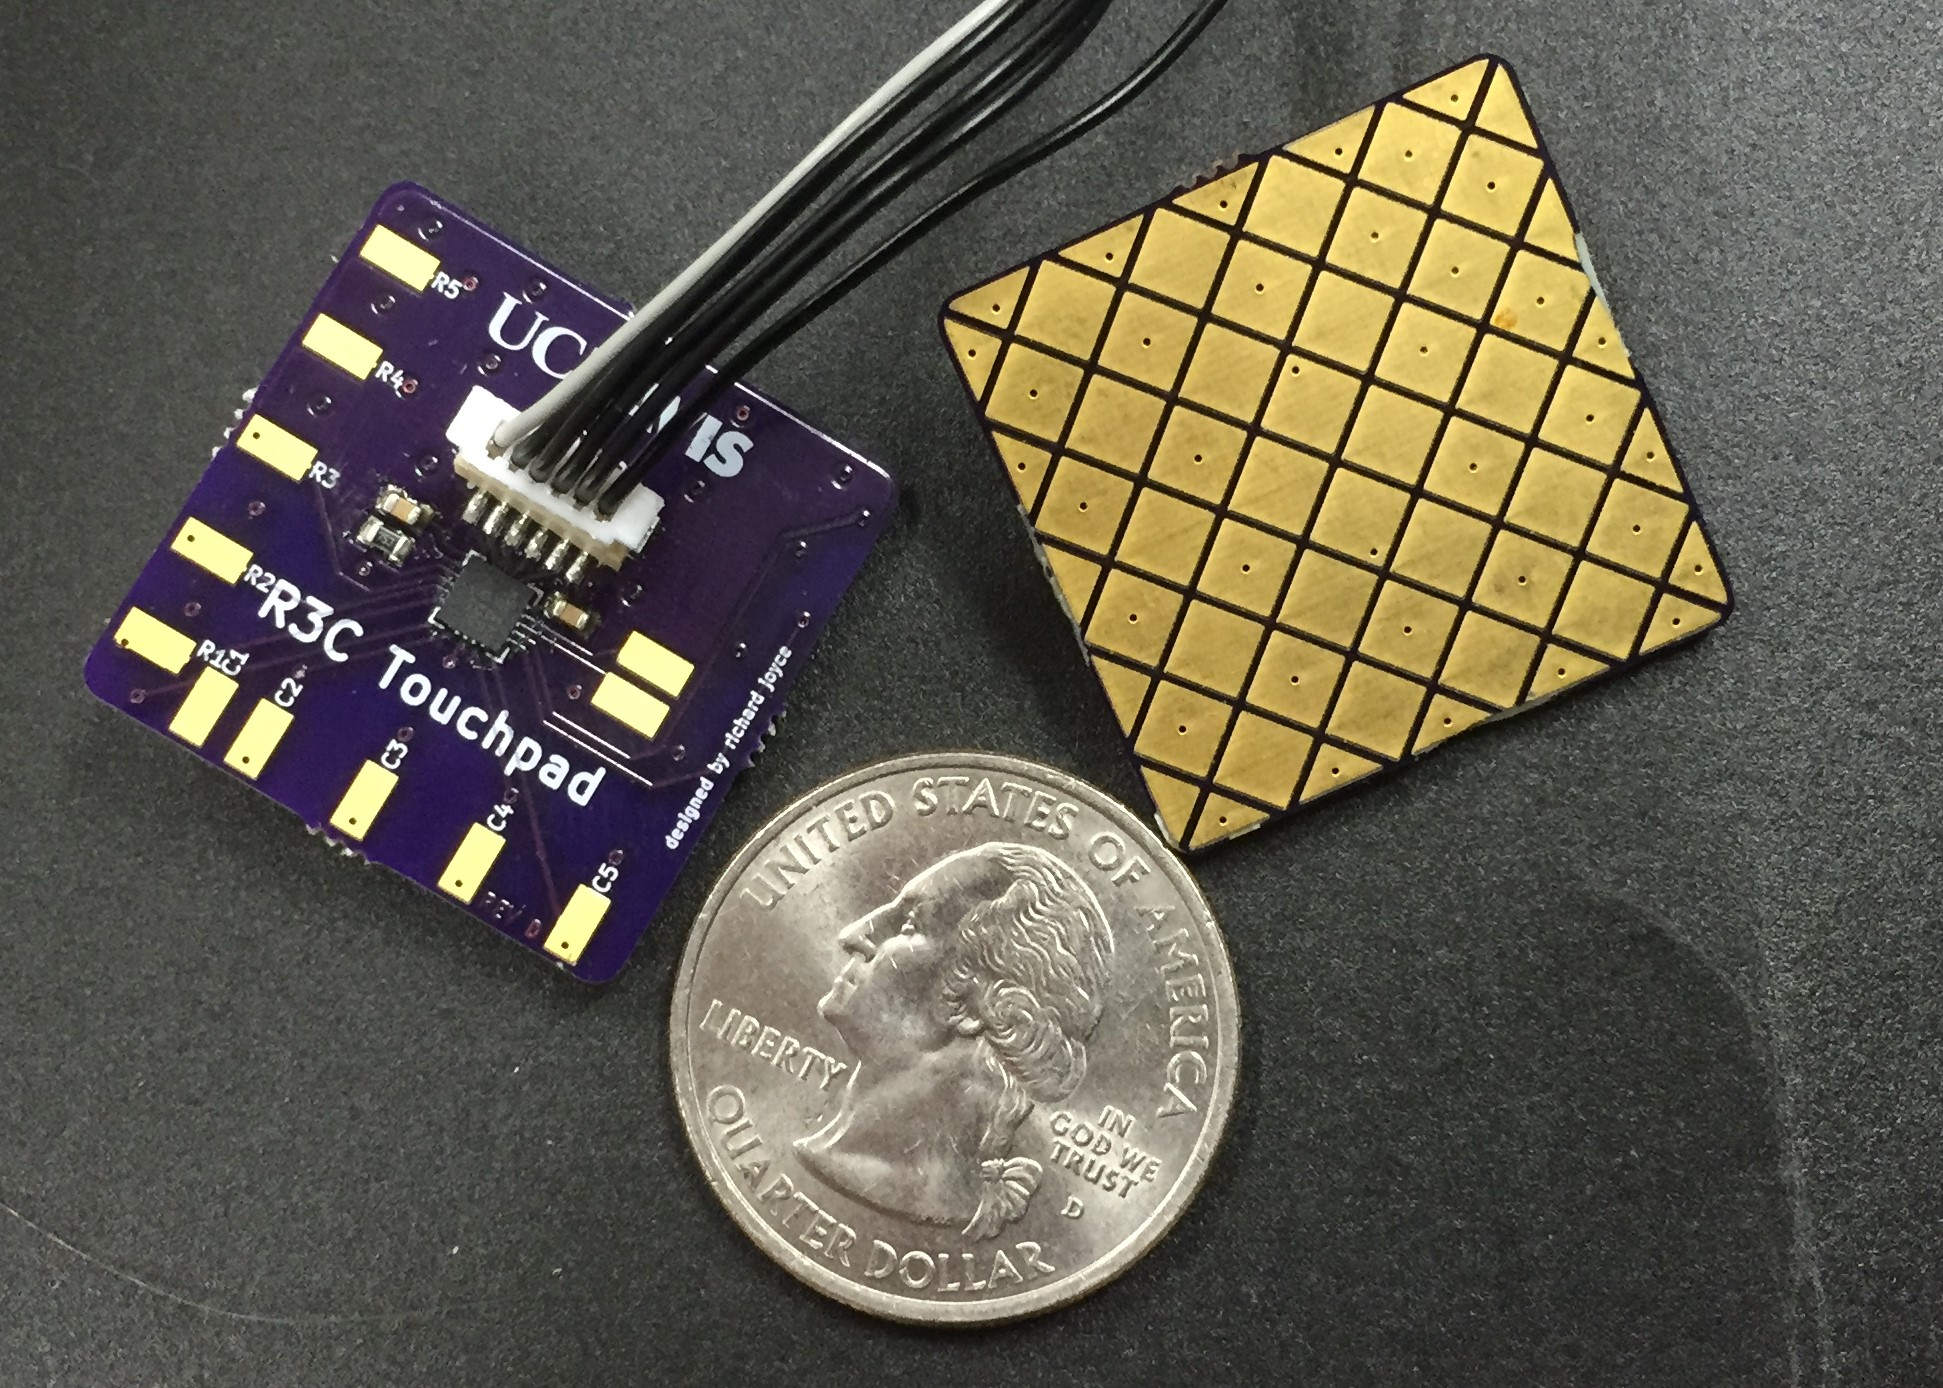
\includegraphics[width=\linewidth]{proto_cap_board.jpg}
    \caption{Bare PCB showing back and front.}
    \label{fig:proto_capacitive_array:pcb}
    \end{subfigure}
    \caption{Capacitive touch array button. Each row and column of diamond pads are connected as one electrode each and together can provide location information of where the user presses.}
    \label{fig:proto_capacitive_array}
\end{figure}

\subsubsection{Calibration}

The hand tracking of the LeapMotion provided precise and repeatable measurement of the hand positions throughout its tracking volume.
The accuracy as the hand got further away from the sensor, however, was insufficient.
Put another way, the position of the hand in the virtual world was offset from the true button position in the physical world, yet the offset was consistent between movements.
This led us to develop a calibration to provide a more accurate registration between the virtual and physical hand positions.
With the addition of the capacitive touch sensors, a calibration mechanism was made possible since it allowed for well known positions in the physical world to be translated to the virtual world.
The location of the buttons are well known from the dimensions of the physical world setup.
This means that when a finger was placed on a physical button with a capacitive sensor, the known position can be recorded along with the ``measured'' position of the hand tracker.
After collecting enough points, the calibration can correct for the measured offset and provide an accurate registration between the real and virtual worlds.
The mathematical basis for this calibration is described here.

The calibration works on the assumption that there exists a transformation matrix, $\mathbf{T}$, that can solve the following equation:
\begin{equation}
    \vec{x}_{known} = \mathbf{T}\vec{x}_{measured}
    \label{eq:proto_Tvec}
\end{equation}
The $\vec{x}_{known}$ and $\vec{x}_{measured}$ correspond to the known location of a calibration point (button) and the location measured by hand tracker, respectively.
Since we know those two vectors, it is only required to solve for the transformation matrix itself.

A simple least squares approach is used to find the coefficients of the matrix. % the registration between the virtual and physical worlds is vastly improved.
The transformation matrix is not constrained to a simple rotation (i.e.\ not assumed orthogonality or other special properties) so the solution is found by expanding and solving the general homogeneous coordinates transformation matrix.
\begin{equation}
    \begin{bmatrix}
        x_{known} \\
        y_{known} \\
        z_{known} \\
        1
    \end{bmatrix} =
    \begin{bmatrix}
        T_{11} & T_{12} & T_{13} &T_{14} \\
        T_{21} & T_{22} & T_{23} &T_{24} \\
        T_{31} & T_{32} & T_{33} &T_{34} \\
        0 & 0 & 0 & 1
    \end{bmatrix}
    \begin{bmatrix}
        x_{measured} \\
        y_{measured} \\
        z_{measured} \\
        1
    \end{bmatrix}
    \label{eq:proto_Tmat}
\end{equation}

Typical least squares approaches would attempt to find $\vec{x}_{measured}$ in Eqn.\ \ref{eq:proto_Tvec}, however we desire to find the matrix $\mathbf{T}$ itself.
It can be shown that expanding the matrix equation (Eqn.\ \ref{eq:proto_Tmat}) for the multiple calibration points (i.e.\ $\vec{x}_{known,1},\dots,\vec{x}_{known,n}$ and $\vec{x}_{measured,1},\dots,\vec{x}_{measured,n}$) and then collecting like terms will convert the problem into three different least squares problems.
They are shown here, dropping the subscripts to $k$ and $m$ for known and measured.

\begin{gather*}
    \begin{bmatrix}
        x_{k1} \\
        x_{k2} \\
        \cdots \\
        x_{kn}
    \end{bmatrix}
    =
    \mathbf{X}_M
    \begin{bmatrix}
        T_{11} \\
        T_{12} \\
        T_{13} \\
        T_{14}
    \end{bmatrix}
    ,\;\;
    \begin{bmatrix}
        y_{k1} \\
        y_{k2} \\
        \cdots \\
        y_{kn}
    \end{bmatrix}
    =
    \mathbf{X}_M
    \begin{bmatrix}
        T_{21} \\
        T_{22} \\
        T_{23} \\
        T_{24}
    \end{bmatrix}
    ,\;\;
    \begin{bmatrix}
        y_{k1} \\
        y_{k2} \\
        \cdots \\
        y_{kn}
    \end{bmatrix}
    =
    \mathbf{X}_M
    \begin{bmatrix}
        T_{31} \\
        T_{32} \\
        T_{33} \\
        T_{34}
    \end{bmatrix}
    ,\\
    \text{where}~\mathbf{X}_M =
    \begin{bmatrix}
        x_{m1} & y_{m1} & z_{m1} & 1 \\
        x_{m2} & y_{m2} & z_{m2} & 1 \\
        &\dots & & \\
        x_{mn} & y_{mn} & z_{mn} & 1
    \end{bmatrix}
\end{gather*}

Now the problem is stated with a known matrix and one unknown vector (per each of the three equations).
Once we have collected more than 4 points, it becomes an over-determined linear system, and a least squares calculation is used to find the solution.
From the solution of the three separate equations, the original $\mathbf{T}$ matrix is reconstructed.

At least 4 points are needed to solve this system, and it has been found that a calibration with small least squares residuals can be achieved with 10-20 well chosen points.
Provided no changes to the lighting or the position of components, the calibration setup can be performed once for the setup and is valid across users.

Instead of using the calibration matrix, $\mathbf{T}$, to transform all of the points in the hand, the index finger was used as the datum for the calibration.
The offset of the index finger between the measured and calibrated positions was calculated and then the entire hand was offset by this vector.
This was done as significant and unrealistic warping would occur with the virtual hand if all points were simply transformed.
This kept the relative position of each joint in the hand as reported by the LeapMotion while calibrating against the point that was most frequently used for button targeting\footnote{Subjects in all research studies were instructed to use their index finger.}.

\subsubsection{Lessons Learned}

The capacitive touch countermeasures were found to be effective, but the visual and aural countermeasures combined with more accurate registration led them to be not needed.
This hypothesis was investigated in the first research study, detailed in Chapter \ref{chap:pointing}.
We often found that a small amount of training time would improve performance.
The observations made were that new users were fixated on placing their finger where the physical feedback indicated the button was and did not adjust for misalignment with the hand tracker, while expert users learned to ignore the physical feedback and activated the hand tracker by finding the misaligned location.
Additionally, we discovered that hand pose and speed can influence the performance of the hand tracker, such that expert users can perform in the system quicker and with greater accuracy.

Not all of the input interactions with a cockpit may be appropriate or possible with just optical tracking.
Some interactions which require a fast reaction time or dynamic input (i.e.\ flight controls) may not be suitable with the current technology.
These insights also get further investigation throughout the research studies, which help quantify which tasks may be appropriate for this system.

We also initially found tracking performance degradation when the finger approached the instrument panel that was due to optical interference with the panel objects (i.e.\ it was happening only when the panel was present).
This was improved when we moved the LeapMotion to the top looking down, but the larger effect was found when looking at the raw image captured by the LeapMotion infrared cameras, discovering our black 3D printed instruments were highly reflective in infrared and showing up the same brightness as the hand.
Applying a matte paint finish improved this, and for future prototypes and configurations the reflections in infrared were monitored.
We have also found better results when covering the entire backdrop of the LeapMotion field of view with a dark matte material, as this helps provide a greater contrast between the hand and the background.

%\tinytodo{more transition}

\subsection{Third Prototype}

The third prototype was developed for the design evaluation experiment.
The motivation for the changes of the third prototype were guided more from research goals than a need for technical improvements of the system.
It is explained in more detail in Chapter \ref{chap:de_exp}, a summary is given here only to describe the technical changes to the prototype.
This premise of this experiment was to understand the utility of the R3C prototype in a design evaluation study.
For this reason, two instruments were designed, modeled, and 3D printed.
Additionally, the experiment required some subjects to use a touchscreen instead of the 3D printed instruments and hand tracker.
The touchscreen was mounted at the same location as the instruments would be (they used the same mounting plate).
The two setups (touchscreen and 3D printed) were interchangeable, and are pictured in Figure \ref{fig:proto_design_exp}.

\begin{figure}
    \centering
    \begin{subfigure}[t]{0.49\linewidth}
        \centering
        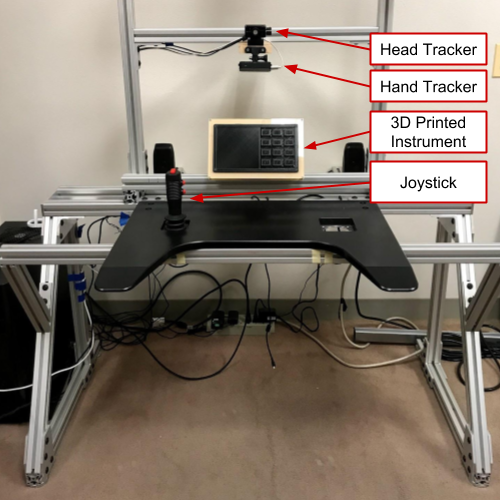
\includegraphics[width=\linewidth]{de_vr_photo.png}
        \caption{VR.}
        \label{fig:proto_design_exp:vr}
    \end{subfigure}
    \begin{subfigure}[t]{0.49\linewidth}
        \centering
        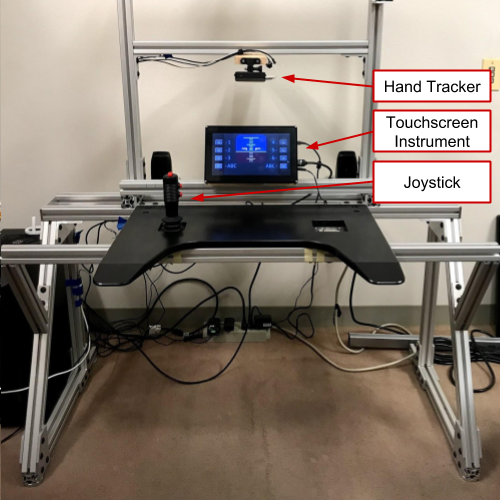
\includegraphics[width=\linewidth]{de_ts_photo.png}
        \caption{TS.}
        \label{fig:proto_design_exp:ts}
    \end{subfigure}
    \caption{Simulator Workstation}
    \label{fig:proto_design_exp}
\end{figure}

With the improvements developed from the previous prototypes, the third prototype was designed to use only the hand tracker to perform input on the 3D printed cockpit instrument buttons.
The hand tracker was mounted above the instrument and pointed towards the area in front of the instrument.
For a more realistic flight simulation, the task also involved using a joystick, which was mounted to the left of subjects at desk height.
To maintain realism, the joystick was modeled in the virtual environment, and moved with the movement of the joystick in the real world.

\subsubsection{Calibration}

The calibration logic was modified for this setup to calibrate based off the position of the touchscreen.
This provided a very accurate and easy way to calibrate the hand tracker.
Instead of using the buttons on the instrument, requiring capacitive touch sensors on the buttons, the calibration was performed by switching to the touchscreen and pressing points on the screen.

One problem that was introduced with the calibration using a touchscreen was that all the points were on a single plane.
The solution to the calibration least squares problem becomes over-fit to the plane, and causes any movement perpendicular to be scaled down near to the plane, causing the hand to appear to be `stuck' to the calibration plane.
To alleviate this, an artificial point was added at 1 inch outward from the middle of the sensor datum.
The same point was added as a known and measured point, forcing the calibration matrix to fit the entire tracking volume instead of just the plane.
This technique came from previous observations which have noticed the accuracy of the sensor was better as the hand was near the tracker.
After solving this issue, the calibration became very accurate with the touchscreen as the data source for known positions.

\section{Summary}

An overview of the technical approach of the evolving Rapidly Reconfigurable Research Cockpit was presented.
The final prototype achieved many of the goals set out by the motivations and requirements.
Developments that were outside the scope of this research work and could be undertaken as future work are discussed in Chapter \ref{chap:conclusion}.
The specific configurations used in each experiment are described in detail within their respective chapter.
Some of the experiments required additional technology development that was not described here as the focus was on the R3C prototype itself.

\chapter{Pointing Experiment}
\label{chap:pointing}

\chapter{Passive Haptics Experiment}
\label{chap:ph_exp}

The first experiment, described in the previous chapter, provided validation that the R3C technology could be used for interacting with a non-functioning mockup.
We found that subjects had a near-perfect success rate using the hand tracking sensor to activate buttons, with accuracy comparable to their performance in a non-virtual environment.
There was a difference in time, with the subjects performing faster in the real, non-virtual environment, and slower in all the virtual environment conditions.
One of the unanswered questions was the effect of the panel as passive haptics on the movement time and accuracy.
The difference in movement time between the subjects using the passive haptics and those without were insignificant.
The main focus of this experiment is the independent variable of passive haptics.
The experimental conditions are reduced from the last experiment to just two: one with passive haptics and one without.
Both conditions are performed with the use of the head-mounted display and the hand tracker.
A more thorough examination of movement time and accuracy is provided by the use of Fitts' Law, and additional dependent measures are also investigated, including presence, learning rate, and trajectory metrics.
This experiment aims to provide a more complete understanding on how the use of passive haptics affects the interaction of a subject with a virtual cockpit panel.
A version of this chapter was presented at the 2017 AIAA Modeling and Simulation Technologies \citep{joyce_passive_2017}.

\section{Introduction}

Passive haptics is a term that has been used to describe a variety of technologies or techniques to provide the sense of touch to a user of a virtual environment.
It is often defined by its distinction from active haptics, which simulate the sense of touch with energy exchange, typically electromechanical.
A common active haptic technology used in immersive virtual environments is a haptic glove, which utilizes small motors at the fingertips.
In contrast, passive haptics often utilize proxy objects placed in the physical world to co-incide with the virtual environment experience.
The proxy objects can be simple or complex.
They can be colocated and accurate with the virtual world or purposefully designed to trick the user.
In our paper, we utilize a simple colocated passive haptic device and measure its effect on the presence and performance of subjects using a 2D panel in a 3D immersive virtual environment.

The advantages to using a simple passive haptic can be easily understood: less cost and complexity compared to most active haptic solutions.
However, the disadvantage comes with its inflexibility.
Due to their nature, passive haptics often have to be purpose built for a single or limited experience.
While past research has aimed to address this, by either actively positioning a proxy object or simplifying the proxy object to fool the user, our application suffers only minimally from this limitation.
The motivation for our research comes from the application of designing aerospace cockpits, complex human-machine interfaces where the user is stationed at their workspace.
For the purpose of evaluating a cockpit design, the user does not need a dynamic tactile environment.
Furthermore, many cockpit design processes already create a physical mockup which can provide the passive haptics for this evaluation.

We present our findings in testing passive haptics versus no haptics in an immersive virtual reality environment.
Using a head-mounted display and a hand tracker, the subjects performed the same Fitts' Law style task under these two haptic conditions.
The passive haptics was a flat surface placed at an angle on a desk in front of their seating area.
Their performance on the Fitts' task was recorded as well as their responses to a presence survey, a self reported arm fatigue score and a general questionnaire.

\section{Background}

\subsection{Haptics}

Passive haptics has been a topic of research since the first immersive virtual environments.
Robotic passive haptics were used to ameliorate the inflexibility of a proxy object by utilizing a robotic arm to position the proxy object in the virtual environment where the user was reaching \citep{tachi_construction_1994,mcneely_robotic_1993}.
%awk
\citet{insko_passive_2001} found that subjects reported increased presence using passive haptics for a maze, and also found that subjects trained with the passive haptics performed better after they were removed than the group that never used them.
Another track of research combined active haptics with passive haptics, using a haptic glove with a physical panel to create mixed haptics \citep{borst_evaluation_2005}.
Again, performance was increased with the haptics, but minimal differences were found between using the mixed haptics and the passive haptics alone.
Similar to our motivation and work, \citet{schiefele_simple_1998} replaced a cockpit panel with a flat panel in an immersive head-mounted virtual environment, and found that users could activate buttons and switches in less time with the panel present than without.
While much of the research involving passive haptics indicates an increase in the presence of the user, some have questioned whether active haptics provides benefits.
\citet{pontonnier_designing_2014} discovered that subjects had decreased presence ratings in a virtual assembly task when using a haptic glove, versus both a real environment and a virtual environment without haptics.
We build on this previous work by investigating the effects of passive haptics with the latest virtual environment technology, as well as performing a complete Fitts' Law characterization between no haptics and passive haptics.

\subsection{Fitts' Law}

Fitts' originally devised a relationship between movement time and the distance and size of targets for a human performing rapid aimed movements \citep{fitts_information_1954}.
This has since become known as Fitts' Law, and later work has refined the index of difficulty ($\mathrm{ID}$) as:
\begin{equation}
    \mathrm{ID}=\log_2\left(\frac{D}{W}+1\right)
    \label{eq:index_of_difficulty}
\end{equation}
where $D$ is the distance to the target from the starting location and $W$ is the width of the target.
This formula for index of difficulty is known as the Shannons' formulation \citep{mackenzie_note_1989}.

Commonly, the index of difficulty is related to movement time ($\mathrm{MT}$) through a linear regression.
However, in this work we are concerned with the measurement known as throughput ($\mathrm{TP}$).
Throughput has been recommended as the dependent measure for comparisons between experimental conditions \citep{soukoreff_towards_2004}.
It can be thought of theoretically as the rate of information the human can input with the particular experimental setup or input device.
It is defined mathematically as the index of difficulty over the movement time, and has the units of ``bits per second'' (\si{\bps}).
\begin{equation}
    \mathrm{TP}=\frac{ID}{MT}
    \label{eq:throughput}
\end{equation}

The use of Fitts' Law as a tool for human-computer interface research began with the research of \citet{card_evaluation_1978} for the evaluation of different input devices for text entry.
The ISO 9241-9 standard was published in 2000 with guidance on using Fitts' Law as an evaluation of pointing devices \citep{international_organization_for_standardization_iso_2000}.
Along with the ISO standard, there have been calls to standardize the use of Fitts' Law so that results can be compared across literature \citep{soukoreff_towards_2004}.
For a 2-dimensional task (where all the buttons exist on a single plane), it is recommended to use the circle layout as shown in Figure \ref{fig:ph_fitts_circle}.
This layout is referred to as the ``Fitts' circle'' within this article.

\begin{figure}
    \centering
    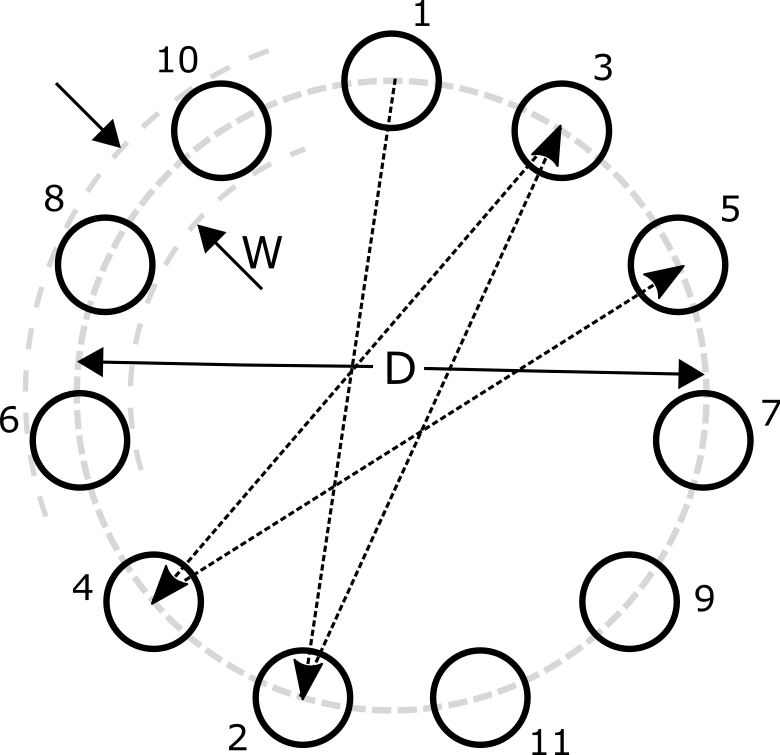
\includegraphics[width=3in]{fitts_circle.png}
    \caption{Fitts' Circle diagram. $D$ is the distance between targets and $W$ is the width of the targets.}
    \label{fig:ph_fitts_circle}
\end{figure}

In this work, we use the effective width for the targets, which is defined as:
\begin{equation}
    W_e = 4.133\sigma
\end{equation}
where $\sigma$ is the standard deviation of the end point positions.
This is known as the adjustment for accuracy \citep{welford_fundamentals_1968}.
This correction accounts for the performance of the subject, especially on lower index of difficulty conditions where they may aim for the inside edge of a target.
Hence, the use of the effective width provides the index of difficulty for the task that the subject performed, not the task presented to them.
The effective width is calculated per subject per distance and width configuration, and subsequently used in the index of difficulty equation.
\begin{equation}
    {ID}_e=\log_2\left(\frac{D}{W_e}+1\right)
\end{equation}

Previous work of evaluating virtual environments and input devices with Fitts’ Law mostly consist of evaluating 3D tasks \citep{chun_evaluating_2004,liu_comparing_2009,teather_evaluating_2010}.
\citet{kohli_redirected_2012} used a passive haptic environment with a head-mounted display, but evaluation focused on their warped virtual space technique.
Recently, some reports have evaluated the Fitts’ performance of the LeapMotion hand tracker \citep{coelho_pointing_2014,seixas_one_2015}, but none have combined hand-tracking with the use of a head-mounted display.

\subsection{Presence}

The feeling of presence is often specified as a goal of a virtual environment.
A definition from \citet{witmer_measuring_1998} reads:
\begin{displayquote}
\textit{Presence} is defined as the subjective experience of being in one place or environment, even when one is physically situated in another.
\end{displayquote}
\citet{sheridan_musings_1992} argued that presence is a subjective sensation that necessitates a subjective measure.
Increased presence has been shown to lead to increased performance in a virtual environment task \citep{youngblut_relationship_2003}.
We use a version of the Presence Questionnaire (PQ) proposed by \citet{witmer_measuring_1998}.
The post-questionnaire consists of 16~questions with a seven-point Likert scale.
\citet{nystad_comparison_2004} found the PQ to be sensitive to technology and interaction methods, so it was chosen to investigate the differences between the two conditions.

\subsection{Arm Fatigue}

Despite the concern of arm fatigue in virtual environments \citep{burdea_virtual_2003}, it was surprising that most results in literature were anecdotal or for mitigation without quantification of the fatigue.
Since fatigue is a subjective quantity, it can be hard to measure it between subjects, and sometimes even within.
The negative impact of arm fatigue on using virtual environments makes it worth investigating.
The arm fatigue scale used within this experiment is a Borg Rating of Perceived Exertion (RPE) scale that ranges from \numrange{6}{20} \citep{borg_borgs_1998}.
\citet{hincapie-ramos_consumed_2014} proposed a model for quantifying and predicting the amount of arm fatigue that correlated well with a Borg scale.
Although there does not exist a standard for arm fatigue measurements in virtual environments, we hope that future researchers will consider including arm fatigue ratings in their experiments.

\section{Methods}

The purpose of the experiment described within this paper is to answer the following research questions:

\begin{enumerate}
    \item Will Fitts' throughput be higher with passive haptics?
    \item Do subjects learn the task more quickly with passive haptics?
    \item What are the differences between the formation of reaching motion trajectories with passive haptics?
    \item Do subjects report less arm fatigue with passive haptics?
    \item Do subjects feel more presence with passive haptics?
\end{enumerate}

\subsection{Experimental Setup}

For the experimental setup, subjects were seated at a desk with a blank panel mounted on an angle in front of them.
The plywood panel (square with length of \SI{18}{\inch}) was used to provide only the backstop of the virtual buttons for the ``Passive Haptics'' condition.
The button selection is registered by the subject moving their index finger into a detection zone (cylinder for the circle buttons) in front of the button that extends outward 0.5in.
Their entrance into the hover zone is indicated to them by the button changing color.
A successful button press is registered after 150ms, and is indicated by the color turning off and a button click noise being played over speakers.

The equipment used consists of an Oculus Rift DK2 (Development Kit 2) head-mounted display (HMD) and a LeapMotion hand tracker.
The low-persistence OLED display of the HMD has a resolution of 1920x1080, with a refresh rate of \SI{75}{\hertz}.
The field of view is approximately \ang{100}.
It utilizes internal sensors (accelerometers and gyros) and an external infrared camera for head tracking.

The LeapMotion is a marker-less hand tracker which utilizes dual infrared cameras to calculate the position of hands and fingers in view.
This position is used to provide an image of the hand position in the virtual environment, as well as for determining when a button is pressed.
Instead of using the LeapMotion in its original face-up configuration, it was mounted above the working area and pointed down.
Our pilot studies (Section \ref{sec:proto-hand-tracking}) indicated that hand tracking from the LeapMotion was improved utilizing this face-down setup with the software using the head-mounted configuration.
However, the hand tracker could not be mounted on the head-mounted display as it required a fixed position relative to the passive haptics to maintain appropriate registration between the virtual world and the passive haptics.

A custom calibration scheme (Section \ref{sec:proto-calibration}) was developed for the hand tracker as the initial registration between physical and virtual worlds was not very accurate.
Despite the pre-calibration inaccuracy, the LeapMotion software was very precise, so after performing the calibration, the registration was kept stable.
The calibration performed a least squares calculation to solve for a transformation matrix between known real world locations and the reported location from the LeapMotion.

\subsection{Experimental Task}

The experimental task was a Fitts' circle in the virtual environment, performed by subjects in two haptic conditions.
The subjects were seated at a desk for the experimental task, and the circle was located on a panel mounted on the desk.
The two haptic conditions were ``No Haptics (NH)'' and ``Passive Haptics (PH).''
These conditions are pictured in Figure \ref{fig:ph_conditions}.
For the ``Passive Haptics'' condition a physical panel was co-located with the panel in the virtual world, and it was removed for the ``No Haptics'' condition.

\mbox{}\hfill
\begin{figure}
    \centering
    \begin{subfigure}[t]{0.3\linewidth}
        \centering
        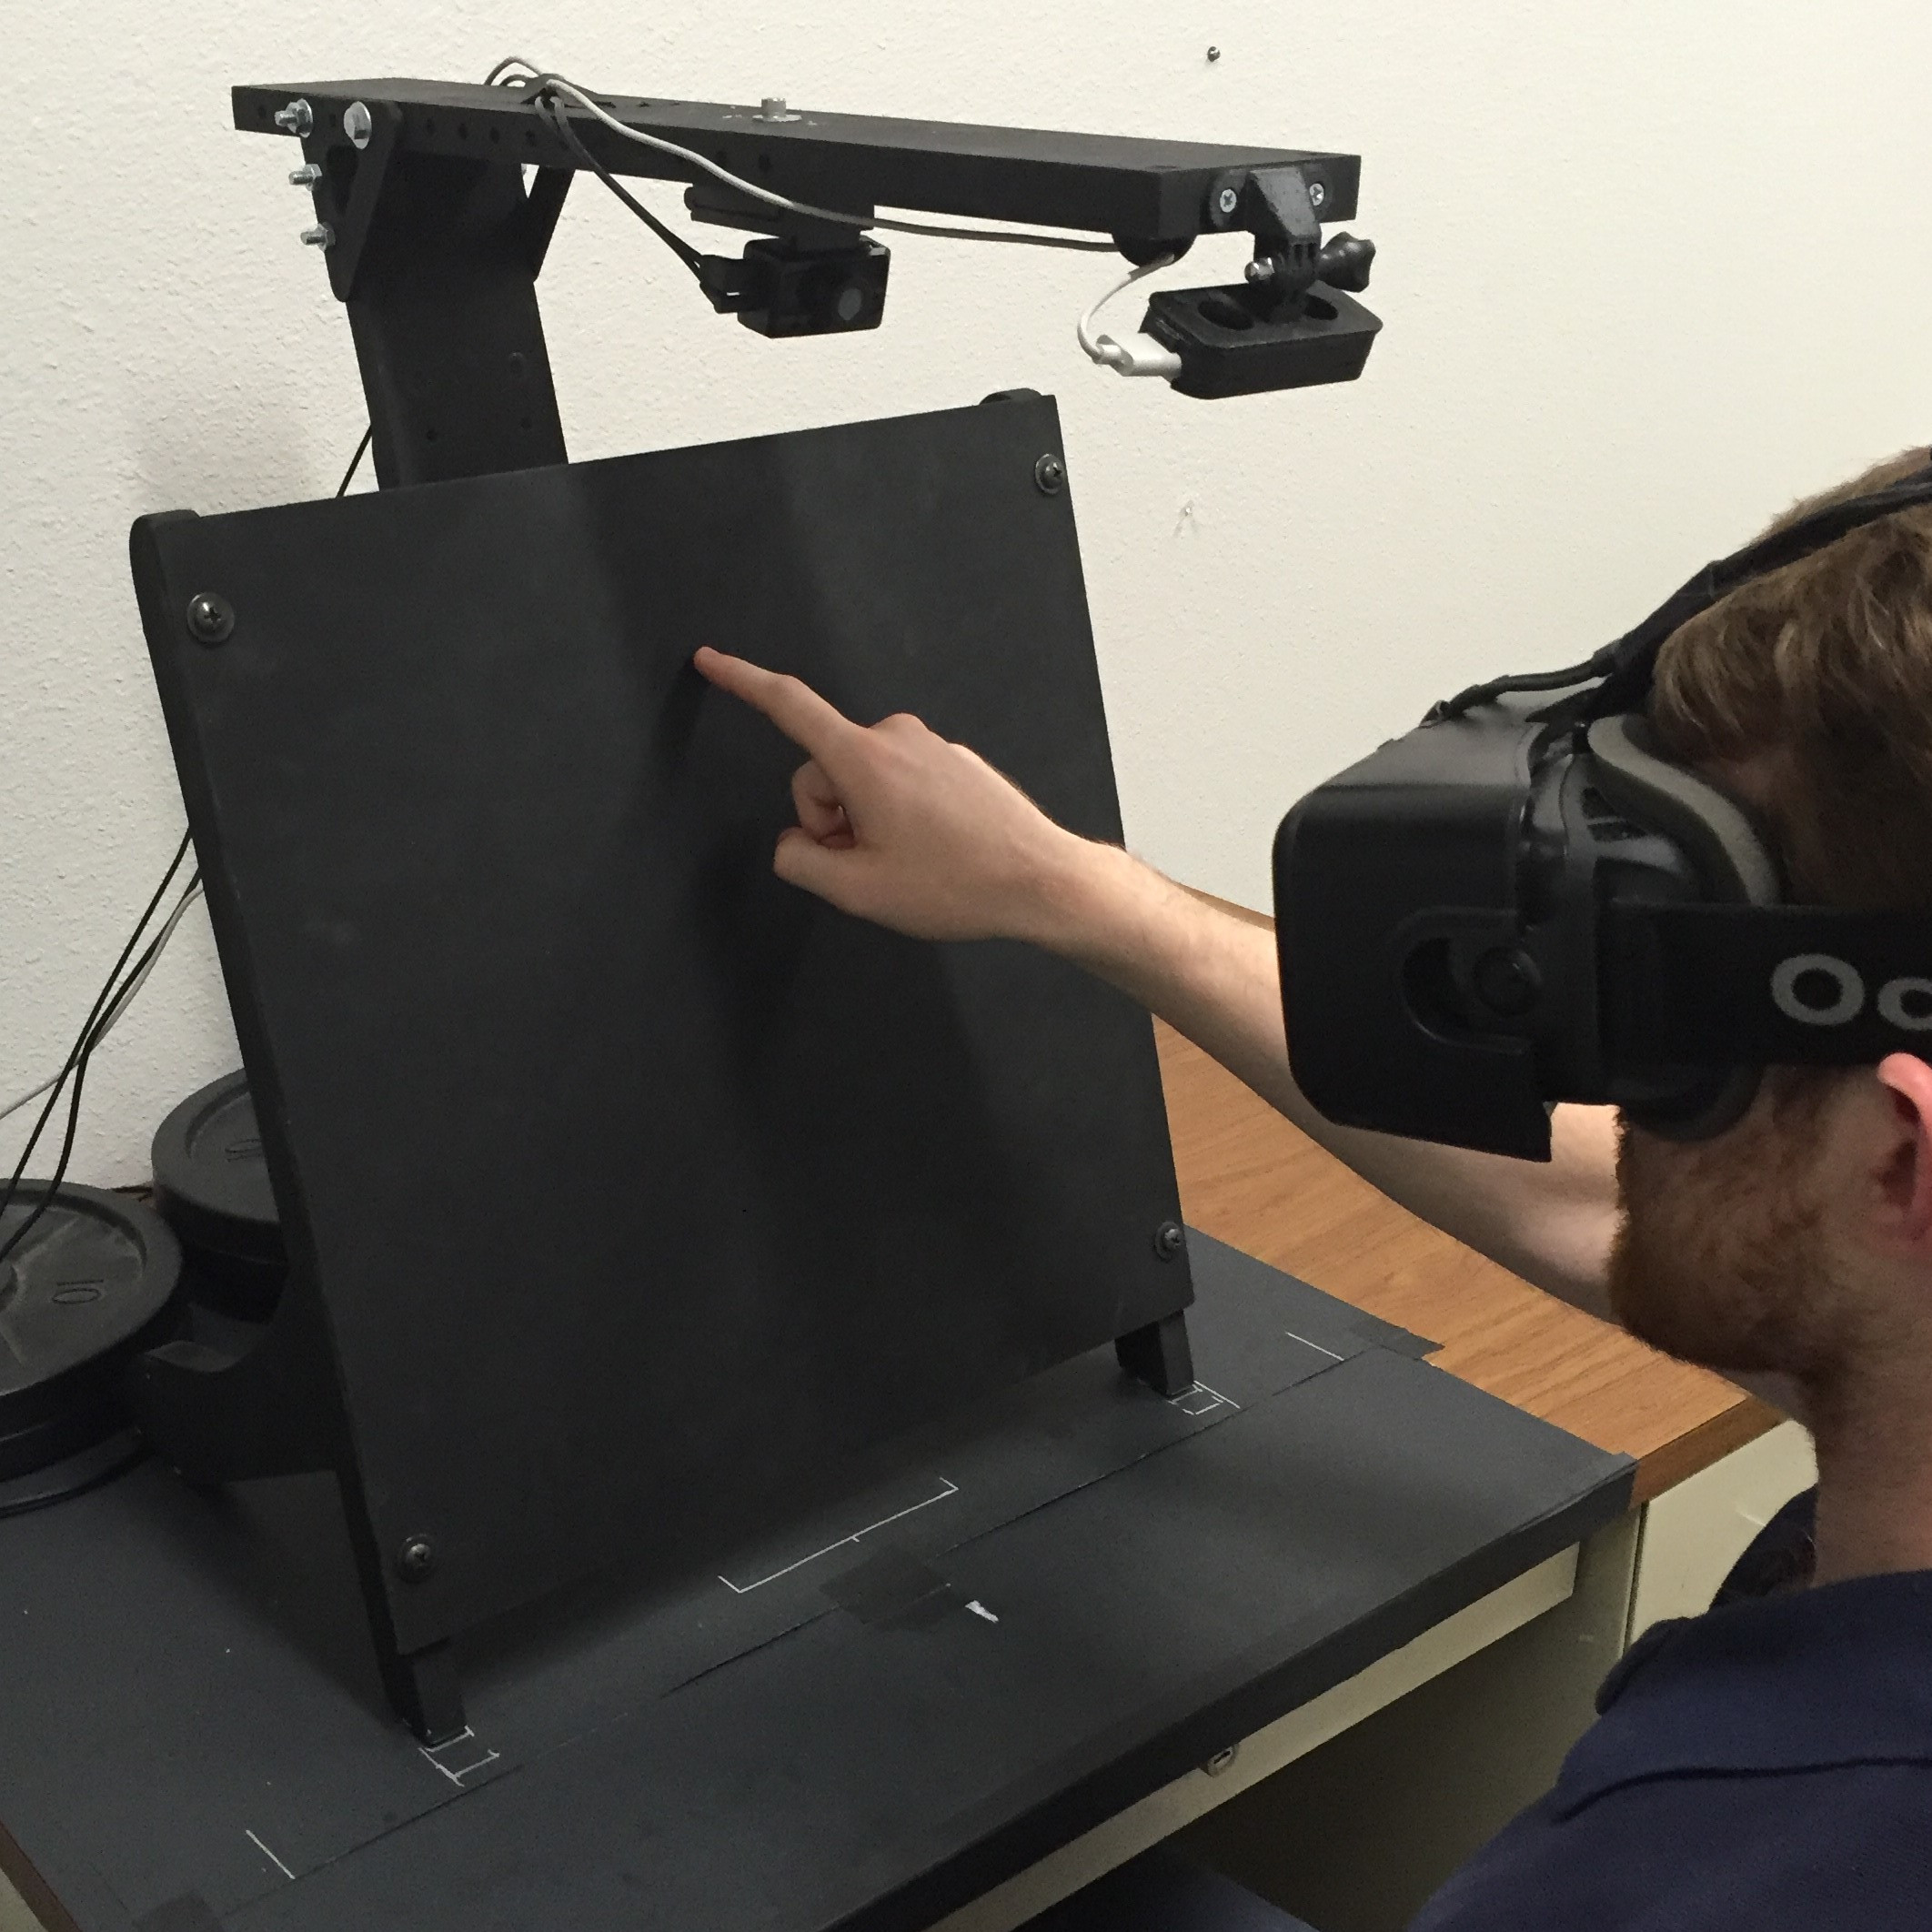
\includegraphics[width=0.9\linewidth]{ph_ph_condition.jpg}
        \caption{Passive Haptics condition (PH)}
        \label{fig:ph_conditions:ph_condition}
    \end{subfigure}\hfill
    \begin{subfigure}[t]{0.3\linewidth}
        \centering
        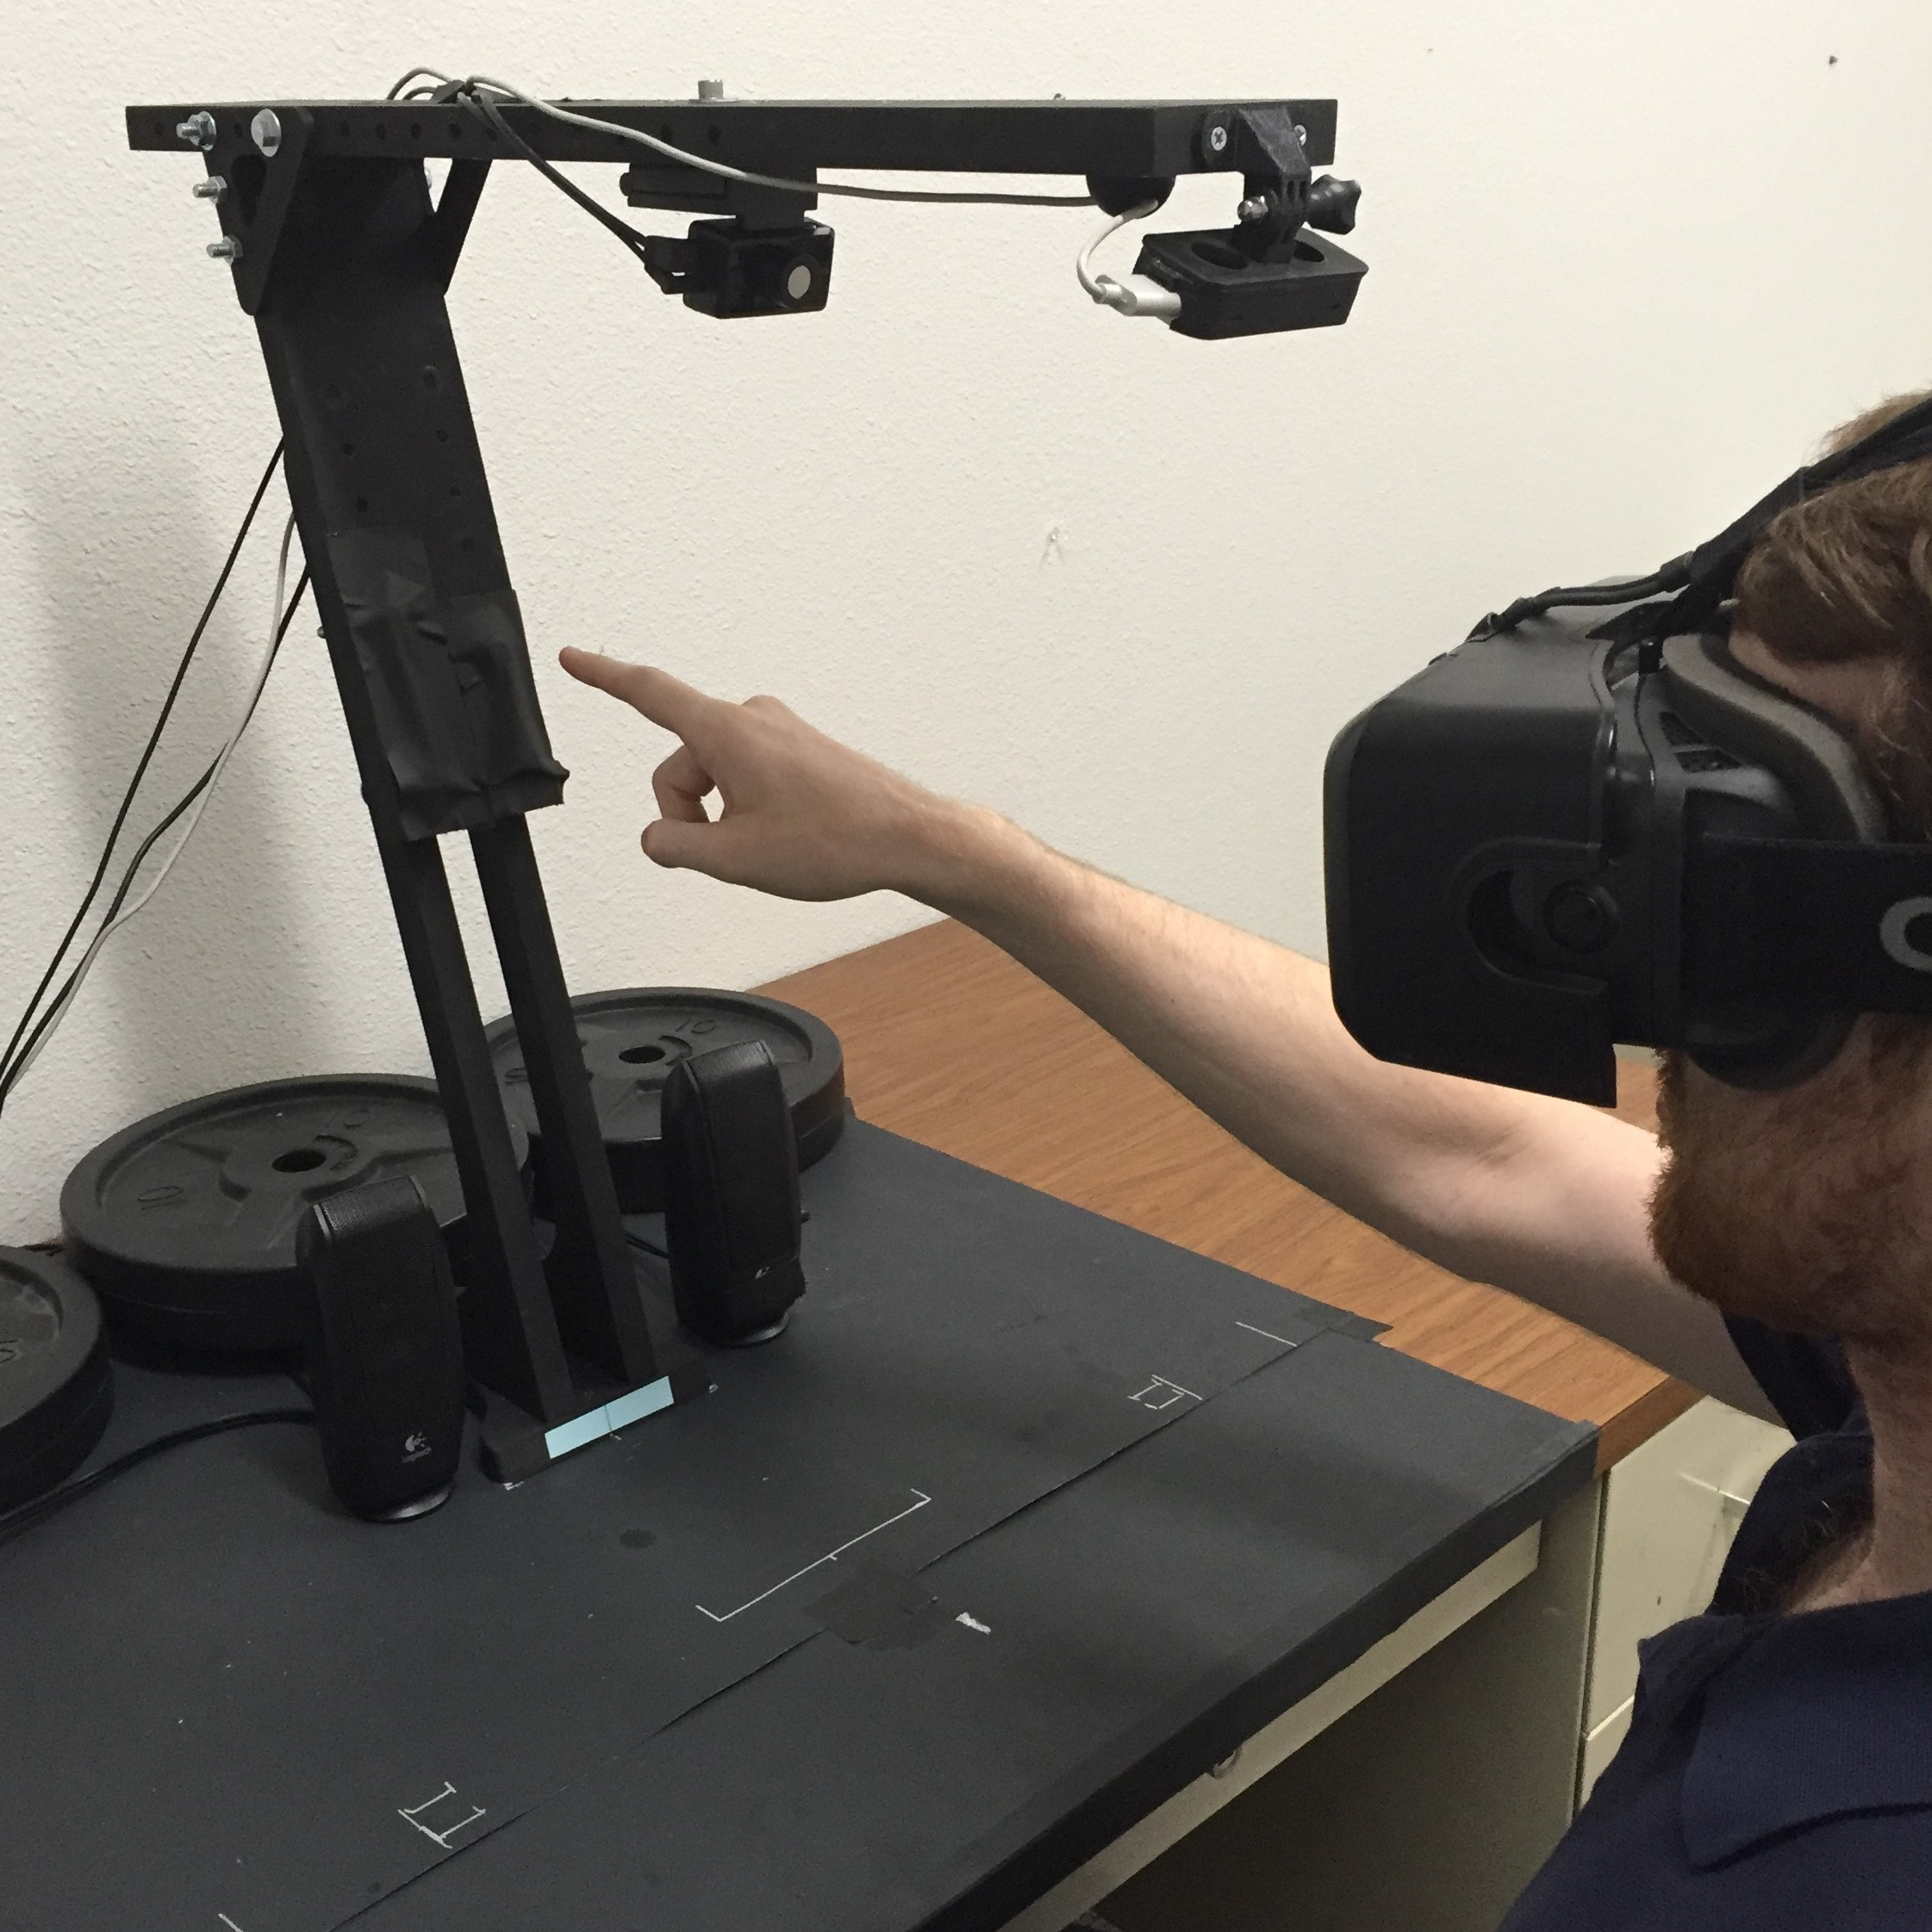
\includegraphics[width=0.9\linewidth]{ph_nh_condition.jpg}
        \caption{No Haptics condition (NH)}
        \label{fig:ph_conditions:nh_condition}
    \end{subfigure}\hfill
    \begin{subfigure}[t]{0.3\linewidth}
        \centering
        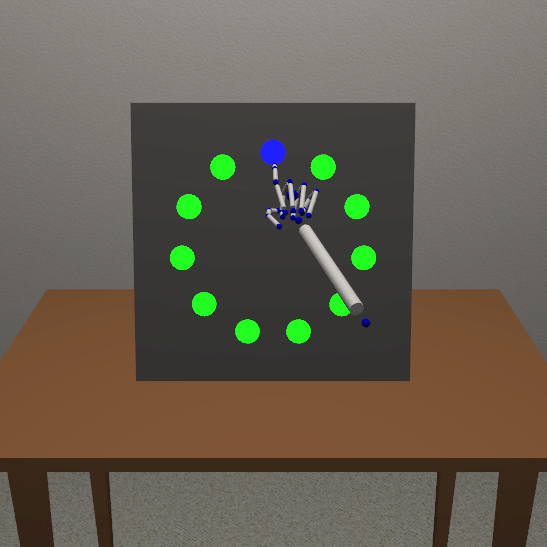
\includegraphics[width=0.9\linewidth]{ph_virtualview.png}
        \caption{View of virtual world (same for both)}
        \label{fig:ph_conditions:virtual}
    \end{subfigure}
    \caption{Experimental conditions and view of virtual environment.}
    \label{fig:ph_conditions}
\end{figure}
\hfill\mbox{}

With the two haptic conditions, there were no differences in the task itself or in the method of button activation.
The only difference between the conditions was the removal of the physical panel.
The hand tracker remained in the same location, preserving the location of the buttons in the virtual environment.
The dimensions of the virtual world were no different for either condition.
In fact, there was no change to the software between the conditions.

Subjects performed the Fitts' circle for three different distances (\SIlist{20;30;40}{\centi\meter}) and five different button widths (\SIlist{5;10;15;20;25}{\milli\meter}).
These configurations were chosen to span a wide range of indices of difficulty (\numrange{3.2}{6.4}).
For each configuration of distance and width, subjects had to complete the full pattern of 11 buttons three times consecutively.
This set of 30 movements\footnote{10 movements between the 11 targets.} for a single configuration is referred to as a single trial for a subject.
The distance was kept constant for the consecutive trials until all five button widths were complete.
The distances were presented in either smallest to largest or vice versa, which was counterbalanced among subjects.

This set of 15 trials was repeated for each haptics condition and the order was kept the same within subjects.
The sequence that the two conditions were presented to each subject was also counterbalanced.
The dependent measures will be tested for interaction with sequence to determine if the results were affected by condition order.

\subsection{Experiment Design}

As described in the previous section, the experiment was performed with a within-subjects design.
Subjects were asked to complete the same experimental task for both conditions of haptics: Passive Haptics (PH) and No Haptics (NH).
The two different haptic conditions are the main independent variables.

We expected significant skill transfer between the two conditions, so the order in which subjects performed the two conditions was counterbalanced.
This created a second independent variable that is between subjects.
The subjects who performed the conditions with the PH being their first condition were one group, and the subjects who performed NH as their first condition were a second group.
We call this grouping ``sequence'' and refer to the two groups as ``PH First'' and ``NH First''.

For a Fitts' Law evaluation, it is often recommended that the data collection only begins when the subject is fully trained on the task.
However, one of the goals of the experiment is to investigate the learning rate of the subjects.
For that reason, the subjects were given no separate training time for the task or virtual environment.
In lieu of collecting the data from fully trained subjects, the throughput analysis will be carried out on movements that are determined to be composed of mostly ballistic motion.
The filtering parameters were determined post-hoc from the trajectory recordings.
Their development and parameter selection are discussed in the results.

\subsection{Dependent Measures}

The main dependent measure is the Fitts' throughput, measured through the movement time between button presses.
Additionally, the trajectory of each movement is recorded from the hand tracker for analysis.
To determine the arm fatigue, subjects were asked to rate their arm fatigue on the Borg scale from \numrange{6}{20}.
The scale was presented with anchors as shown in Appendix \ref{sec:app_ph_exp} (Table \ref{tab:ph_borg_scale}).
The arm fatigue rating was collected at the beginning of each condition, and then after every other configuration of distance and width combination (and after the final trial due to an odd number of trials).
At the completion of each condition the subject was given a presence questionnaire.
At the end of the experiment, an additional condition comparison survey was given to ask for opinions on the two haptic conditions.

\subsection{Trajectory Phases}
\label{sec:ph_traj_phases}

Human reaching movements have long been known to consist of two distinct phases \citep{woodworth_accuracy_1899}: a ballistic phase and a corrective phase.
The ballistic phase is an open-loop, gross adjustment towards the target, while the corrective phase is more refined movement honing in on the target.
To separate the trajectories into the various phases, a simple algorithm was developed.
First, the local minima are found throughout the velocity profile of the movement to separate the movement into various submovements.
The ``ballistic phase'' is then classified as the submovement which contains the peak velocity of the entire movement.
The various submovements after the ballistic phase are classified as the ``corrective phase''.
Any movement before the ballistic phase is classified as a ``reaction time''.
An example of the results of this classification is shown in Figure \ref{fig:ph_trajectory_ballistic}.
This mathematical definition does break down for certain cases where a subject might have two submovements in the ballistic phase due to a mid-course correction or similar, however one of the main purposes of this classification for this experiment was to find movements which are appropriate to use for the Fitts' Law calculations.
Therefore, movements with multiple submovements are likely to not be ballistic, well-learned movements.


\begin{figure}
    \centering
    \includegraphics[width=4.0in]{{trajectory_velocity.ballistic}.png}
    \caption{Example trajectory with three phases indicated.}
    \label{fig:ph_trajectory_ballistic}
\end{figure}

\subsection{Trajectory Filtering}

We used a low-pass filter on the trajectory recordings to reduce the amount of noise.
The LeapMotion processes data at a variable frequency, thus creating a variable rate for recording.
The frequency typically varies from about \SI{100}{\hertz} to \SI{120}{\hertz}.
To perform the filtering, the data was first resampled to a fixed rate of \SI{100}{\hertz}.
The filter used is a fourth-order Butterworth filter with a cut-off frequency of \SI{5}{\hertz}.
The cut-off frequency was chosen as voluntary hand movements have been shown to be below such a rate \citep{riviere_toward_2003}.

\section{Results}

\subsection{Participants}

Twenty (20) subjects were recruited from the UC Davis engineering student population, both undergraduate and graduate students.
The age range was \numrange{19}{29} ($M=23.0, \sigma=3.0$) with 16 males and 4 females.
The genders were balanced among the counterbalanced sequence groups.
All subjects indicated either less than one hour or no prior experience with virtual reality.
The total time spent in the experiment was under one hour, with a range of approximately ten to twenty minutes performing each of the two conditions in virtual reality.

\subsection{Throughput}

The throughput is calculated per movement using Equation \ref{eq:throughput} and meaned per trial before being meaned per subject and condition.
Throughput is used to investigate the first two research questions: do the subjects learn more quickly and does their throughput performance improve with passive haptics?

\subsubsection{Rate of Learning}

\begin{figure}
    \centering
    \includegraphics[width=\textwidth]{{throughput_trials.8.0x4.0}.png}
    \caption{Throughput per trial. The learning curve exponential fit is given by Eq.~\ref{eq:ph_learning} with parameters from Table \ref{tab:ph_tp_regression}.}
    \label{fig:ph_throughput_trials}
\end{figure}

The average throughput for each trial, separated by haptics condition, is shown in Figure \ref{fig:ph_throughput_trials}.
An exponential rise to a learned state is fit to each haptics condition to model the learning curve of the subjects.
The equation used is given as:
\begin{equation}
    \mathrm{TP}(T) = \mathrm{TP}_{\infty} - (\mathrm{TP}_{\infty}-\mathrm{TP}_0)e^{\left( -T / \tau \right)}
    \label{eq:ph_learning}
\end{equation}
where $T$ is the trial number, $\mathrm{TP}_{\infty}$ is the asymptotic learned value of throughput, $\mathrm{TP}_0$ is the initial value at $T=0$ and $\tau$ is the time constant.
The time constant is defined as the number of trials for the throughput to rise 36\% of the difference between the fully learned throughput ($\mathrm{TP}_{\infty}$) and the initial throughput ($\mathrm{TP}_0$).
The parameters of the fit for each condition is shown in Table \ref{tab:ph_tp_regression}, as well as the standard error of the estimate (SEE).
The value of throughput from the regression fit as a percentage of the fully learned value ($\mathrm{TP}_{\infty}$) for representative trials are listed in Table \ref{tab:ph_tp_regression_values}.

The rate of learning is very similar among both groups in the first condition.
For the first condition it can appear that the subjects performing NH learned more quickly than their counterparts performing PH by looking at the time constants.
However, as the values in Table \ref{tab:ph_tp_regression_values} show, the NH First group started their first trial at a lower percentage of their learned state.
The shape of the learning curves are very similar and both groups reached approximately 90\% of their fully learned state by the 5\textsuperscript{th} trial.

The learning curves are quite different for the second condition.
The NH condition does not have a learning curve at all, with a straight line being a better fit than the exponential function.
This indicates the transfer of training from the PH condition allowed the group who did PH first to immediately perform in NH at the same level as the fully learned state of the subjects who learned NH in their first condition.
This transfer of training to the second condition did not occur as strongly for the group who did NH first.
Their initial performance of PH did start out at a slightly higher level than the subjects who did PH first (\SI{2.8}{\bps} vs \SI{2.4}{\bps}), but after 5 trials this difference had converged (\SI{3.6}{\bps} vs \SI{3.7}{bps}).

\begin{table}
    \centering
    \includetable{throughput_regressions.tex}
    \caption{Exponential fit parameters of Eq. \ref{eq:ph_learning}. Curves are shown in Figure \ref{fig:ph_throughput_trials}. $\mathrm{TP}_{\infty}$ is the asymptotic learned value of throughput. $\mathrm{TP}_0$ is the initial value at trial~0. $\tau$ is the time constant of the exponential function. SEE is the standard error of the estimate for the fit.}
    \label{tab:ph_tp_regression}
\end{table}

\begin{table}
    \centering
    \includetable{throughput_regression_values.tex}
    \caption{Percentage of fully learned state for various trials for each group and condition from learning model fit. $\mathrm{TP_i}$ is $\mathrm{TP}(i)/\mathrm{TP}_{\infty}$ using Eq. \ref{eq:ph_learning}. Trial 15 is the final trial for each condition.}
    \label{tab:ph_tp_regression_values}
\end{table}

These results indicate that subjects did not learn faster with Passive Haptics.
The only differences between learning rates is the positive transfer of training from performing Passive Haptics first followed by No Haptics second.
The answer to the research question \textit{Do subjects learn the task more quickly with passive haptics?}\ appears to be that the passive haptics does not make subjects learn faster, but they are able to learn the task more quickly without passive haptics afterward.
It does appear that the fully learned state is different between the haptic conditions, which is investigated through the use of throughput after discussing data filtering.

\subsubsection{Ballistic Movement Filtering}
\label{sec:ph_ballistic_filter}

Before they could be used for the Fitts' Law analysis, the trajectories were filtered so that only movements which were direct to target were included.
A well-learned movement appropriate for Fitts' Law is one which moves directly towards the target and does not have much extraneous movement or idle time beyond what is required to complete the task.
As a result of the experiment design and questions requiring subjects to learn the task during the data collection, we expected many of the movements to deviate from a well-learned movement.
% awk
During the observation of subjects during the experiment, as well as post-hoc examination of the dataset, a number of common patterns were discovered and targetted by the filters in this section.
The goal of this filtering is to produce a dataset that only includes the direct to target movements approriate for a Fitts' Law analysis for the final throughput calculations.
We describe in this section the three metrics developed that were used to determine whether a movement was direct to target.

%An inordinate amount of time was spent either in the reaction phase before the ballistic, or more typically, after the ballistic movement in the corrective phase.
%There were two common causes of a long time spent in the corrective phase, the first was that the subject had trouble finding the activation zone or holding it there for the 160 msec required.
%The second cause was that the subject would have a false start and move towards the next target before their button press was activated.
%For the former, this led to a increase in time for the corrective phase, but not neccesarily a large path distance increase.

%To perform the filtering, three metrics were developed.
The first metric was the ratio of path distance traveled in the ballistic phase to the distance between the targets for that movement (i.e. \SIlist{20;30;40}{\centi\meter}).
Ideally, the ballistic portion would cover the majority of the distance between the targets.
A movement which covered too little of the target distance could mean the subject slowed or stopped in the middle of movement, and one that covered more could mean the subject overshot or had an indirect trajectory.
A sample movement that gets flagged by this filter is shown in Figure \ref{fig:ph_traj_filter_target}, which has a ratio of 1.49.
This is an example of a movement that does seemingly have a direct movement toward the target, but includes a large deviation perpendicular to the movement axis.
This deviation could mean the subject initially aimed their ballistic portion in the wrong direction but performed a correction during the movement.
The limits for this filter were chosen as having a ratio between 0.90 and 1.10, i.e.\ within 10\% of the target distance.
This filtered out 4577 of the 17970 movements (25.5\%).

\begin{figure}
    \centering
    \includegraphics[width=4.0in]{{trajectory_both.bad_target_filter}.png}
    \caption{An example of a movement with a large ballistic distance to target distance ratio. The bottom plot shows the projection of the trajectory on the plane of the Fitts' circle.}
    \label{fig:ph_traj_filter_target}
\end{figure}

The second filtering metric was also based on the ballistic phase path distance.
For this metric the ballistic phase path distance was compared to the total path distance the subject traveled for their entire movement.
This filter targeted movements where, after the ballistic phase, the subject moved away from the target, or had a smaller but significant movement before the main ballistic movement.
An example is shown in Figure \ref{fig:ph_traj_filter_distance} which shows a movement which passed the first metric (the ballistic phase distance ratio to the target distance was 1.03), but the ballistic phase was only 56\% of the total distance traveled during that movement.
This was a common problem where a subject would have a false start for the next target and move away from the current target before their button press was activated.
The threshold for the filter was set at 0.80, which rejects 4264 movements that are lower than the threshold.
Of the rejected movements, only 1675 were unique from the rejected movements of the previous target distance filter.
Between the two filters so far, there have been 6252 of the 17970 movements filtered out (34.8\%).

\begin{figure}
    \centering
    \includegraphics[width=4.0in]{{trajectory_both.bad_distance_filter}.png}
    \caption{An example of a movement with a small ballistic distance to total path distance ratio. The bottom plot shows the projection of the trajectory on the plane of the Fitts' circle.}
    \label{fig:ph_traj_filter_distance}
\end{figure}


The last filter took a time based approach, and looked at the ratio of the time spent in the ballistic phase over the total movement time.
This filter removed movements where the subject spent an inordinate amount of time either before or after the ballistic phase.
If they were not moving during the non-ballistic phases, it would not have been caught by the distance-based filters either.
The threshold of 0.40 meant that 4496 movements were filtered, however only 873 of those are unique of the other two filters.
Figure \ref{fig:ph_traj_filter_time} illustrates a movement where the subject waited before initiating the ballistic movement.
Since the subject did not move during this idle time, the other two filters did not flag this movement.

\begin{figure}
    \centering
    \includegraphics[width=4.0in]{{trajectory_both.bad_time_filter}.png}
    \caption{An example of a movement with a small ballistic time to total time ratio. The bottom plot shows the projection of the trajectory on the plane of the Fitts' circle.}
    \label{fig:ph_traj_filter_time}
\end{figure}

The combination of these three filters led to 7125 of 18000 movements being filtered out, leaving 60.4\% of the movements.
For each of the metrics, the threshold was determined by investigating the distribution and looking at sample movements on either end of the threshold to determine if it was an appropriate value.

The final check before performing the Fitts' calculation was to ensure that each trial had enough data for the adjustment for accuracy calculation.
The adjustment for accuracy is based on the distribution of endpoint data from a single trial (which is one distance and width configuration).
One trial consists of 30 consecutive movements, but the ballistic filtering could diminish the amount remaining in each, so a trial was only included if at least half (15 of 30) of the movements were considered to be good movements by the ballistic filters.
This means that movements from a trial that did not have enough good movements were also filtered out from the Fitts' calculation.
Not only is this important to make sure the adjusted width is valid, it also removes trials where the subject likely did not reach a fully learned state, as most of their movements were not primarily ballistic movements direct to target.
On average, 11 of 15 trials per condition from each subject ($M=10.98, \sigma=3.25$) had enough good movements to be included.
This left 9218~movements for the Fitts' calculation, just over half of the total movements (51.3\%).
Slightly more movements were filtered from the No Haptics condition, with 47.1\% of NH movements left after the filtering, compared to 55.5\% of the PH movements.
For the remaining sections, unless otherwise noted, the results were based on using only the movements after filtering.

\subsubsection{Throughput}

The throughput was found to be higher in the PH condition, at \SI{4.25}{\bps} compared to the \SI{3.76}{\bps} of the NH condition.
A two-way mixed ANOVA was performed to determine the effect of haptics condition.
Since we expected order effects, and have seen them with the transfer of training seen in the Rate of Learning section, the sequence the subjects performed the haptic conditions was included as a between subjects factor.
The effect of haptics was found to have a significant effect on the throughput ($F(1,18)=35.59, p<0.001$) between the PH condition ($M=\SI{4.25}{\bps}, \sigma=\SI{0.44}{\bps}$) and the NH condition ($M=\SI{3.76}{\bps}, \sigma=\SI{0.38}{\bps}$).
There was no effect on throughput based solely on sequence group ($F(1,18)=0.53, p=0.47$), but there was a marginally significant interaction effect between the sequence and haptics ($F(1,18)=4.48, p=0.048$).

As can be seen in Figure \ref{fig:ph_throughput}, this marginal interaction effect appears to indicate that both groups had improved performance but that the PH First group performed better at the NH condition.
A post-hoc repeated measures t-test between haptic conditions for the subjects who performed PH First was significant ($t(9)=4.62, p<0.001$), with the PH condition ($M=\SI{4.23}{\bps}, \sigma=\SI{0.34}{\bps}$) outperforming the NH condition ($M=\SI{3.91}{\bps}, \sigma=\SI{0.40}{\bps}$).
The mean of the differences between subjects was \SI{0.32}{\bps}.
The group of subjects who performed NH first also had a significant effect in the t-test ($t(9)=3.96, p<0.001$) between the PH condition ($M=\SI{4.28}{\bps}, \sigma=\SI{0.54}{\bps}$) and the NH condition ($M=\SI{3.62}{\bps}, \sigma=\SI{0.32}{\bps}$).
There was a higher mean of differences (\SI{0.66 }{\bps}) with the NH First group than the PH First group.
These post-hoc tests confirm that both groups had a significant effect of haptics, though the NH First group had a larger difference between the conditions.

\begin{figure}
    \centering
    \includegraphics{{throughput.4.0x4.0}.png}
    \caption{Throughput boxplot by haptics and sequence.}
    \label{fig:ph_throughput}
\end{figure}

It is worth noting that without using the ballistic filter, the major conclusions found do not change.
The only major difference is the magnitude of the throughput and size of the differences.
The statistical tests have the same results as well.
The results by haptics for both filtered and unfiltered are shown in Table \ref{tab:ph_throughput_fulltable}.
These results indicate that subjects do have higher throughput with passive haptics, answering our first research question.

\begin{table}
    \centering
    \includetable{throughput_fulltable.tex}
    \caption{Throughput scores by haptics condition.}
    \label{tab:ph_throughput_fulltable}
\end{table}

% Factors causing this.

% Counts of the filters

\subsection{Trajectory Phases}

As described in Section \ref{sec:ph_traj_phases}, each movement of the subjects can be dissected into three distinct phases: reaction time, ballistic phase, and corrective phase.
We have already seen that, overall, the subjects took more time to complete a movement without the passive haptics in place.
In this section we investigate the differences in time spent in the three phases.
We report here the means of time spent in each of the three phases.
Times reported are all milliseconds.
The results are shown for the filtered and unfiltered results, where the filtered results only include movements that were deemed primarily ballistic by the filtering methods in Section \ref{sec:ph_ballistic_filter}.
The unfiltered results include all movements.
The phases were meaned per subject first, and then by condition.
The time spent in each phase is listed in Table \ref{tab:ph_phases}.
Each phase was tested for the effect of haptics and sequence through a mixed two-way ANOVA.
The statistical tests reported here are for the filtered results, but the significance findings do not change between filtered and unfiltered.

The reaction time was not significantly affected by the presence of haptics ($F(1,18)=0.32, p=0.58$) or sequence ($F(1,18)=0.001, p=0.98$).
However, for the interaction between the two a significant effect was found ($F(1,18)=18.56, p<0.001$).
The interpretation of this interaction effect without main effect significance is that the first and second condition had a different reaction time, without dependence on the haptics condition or group.
The mean reaction time in the first condition for both groups was \SI{130.9}{\milli\second} ($\sigma=\SI{41.0}{\milli\second}$), but in the second condition it was just over \SI{20}{\milli\second} faster, with an average of \SI{109.1}{\milli\second} ($\sigma=\SI{36.6}{\milli\second}$).
The reaction time for both conditions was lower than generally accepted values for reaction time to a visual or aural stimulus \citep{teichner_recent_1954}.
This is not surprising, as the task was a serial task which the subjects would learn the pacing of throughout the experiment.
It would be expected that they were able to learn to anticipate the activation of a button (which was also the start of the next movement) as it would activate \SI{150}{\milli\second} after the subject entered the zone of the previous button.
This interaction effect indicates that subjects did learn how to anticipate the activation event independent of the haptics or the order they performed the conditions.
%When including all the movements in the unfiltered case, the reaction time also has no significance due to the effect of haptics or sequence, but it .
%It also does not have a significant interaction effect, which is not surprising as the unfiltered movements were un

The ballistic phase time had a significant effect of haptics ($F(1, 18)=24.14, p<0.001$) between PH ($M=\SI{772.6}{\milli\second}, \sigma=\SI{67.7}{\milli\second}$) and NH ($M=\SI{719.5}{\milli\second}, \sigma=\SI{60.0}{\milli\second}$).
There was no effect of sequence or the interaction effect between haptics and sequence.
Since the ballistic phase should be mostly independent of the use of passive haptics, it was not expected to see the ballistic phase have an effect of haptics.
It is unclear the exact mechanism that led to this, but it could be an artifact of the passive haptics causing the subjects to learn the movement, and thus allowing them to move more quickly.
The difference between the two haptic conditions was small in magnitude (\SI{53}{\milli\second} or 7\%), so this may not be a practical significance.
There is little difference between the filtered movements and unfiltered movements results, the difference of the means were within a few milliseconds.
Although the ballistic phase had lower movement times with the unfiltered movements, this is due to including movements where the ballistic was not the complete movement, reducing the mean.

The corrective phase time also had a significant effect of haptics ($F(1, 18)=22.46, p<0.001$) between NH ($M=\SI{256.6}{\milli\second}, \sigma=\SI{42.1}{\milli\second}$) and PH ($M=\SI{199.1}{\milli\second}, \sigma=\SI{48.1}{\milli\second}$).
There was no effect of sequence or the interaction effect between haptics and sequence.
This result was expected as one of the main benefits of the passive haptics is that the subject does not have to `find' the target along one dimension.
There was a more noticeable difference between the results of the unfiltered and filtered movements for the corrective phase.
The corrective phase time was much higher in both conditions for the unfiltered, with PH having a mean of \SI{564.7}{\milli\second} ($\sigma=\SI{253.6}{\milli\second}$) and NH having a mean of \SI{837.2}{\milli\second} ($\sigma=\SI{293.2}{\milli\second}$).

This answers our third research question \emph{What are the differences between the formation of reaching motion trajectories with passive haptics?}.
The analysis finds that the most notable difference is that subjects spend significantly less time in the corrective phase with the passive haptics.

\begin{table}
    \centering
    \includetable{phases_fulltable.tex}
    \caption{Time in each movement phase by haptics conditions.}
    \label{tab:ph_phases}
\end{table}

\subsection{Arm Fatigue}

The subjects were asked for a rating of their arm fatigue every other trial, as well as before the first trial and after the last trial of each condition.
One trial lasted for 30~movements and consisted of a single distance and width configuration.
The scale ranged from \numrange{6}{20}, and subjects were allowed to record decimal ratings.
The full scale with anchors are shown in Appendix \ref{sec:app_ph_exp} (Table \ref{tab:ph_borg_scale}).
The average rating at each trial, separated by haptics condition, is shown in Figure \ref{fig:ph_armfatigue_trials}.

\begin{figure}
    \centering
    \includegraphics[width=\textwidth]{{armfatigue_trials.8.0x4.0}.png}
    \caption{Arm Fatigue by Trial.}
    \label{fig:ph_armfatigue_trials}
\end{figure}

There is an evident difference between the two haptic conditions for the first condition performed, with the NH condition subjects accumulating more fatigue throughout the trials.
At the end of the first condition, the subjects who performed the PH condition rated their arm fatigue 3.25~points lower on average than the NH condition subjects.
Both groups have a similar rate of recovery, but the second condition quickly converges and shows no apparent difference between the two haptics conditions.

A within-subjects repeated measure (haptics) with two between-subjects measures (sequence and trial) ANOVA was performed to test the significance of haptics and the interaction effect of haptics and sequence.
The interaction effect of haptics and sequence was found to be significant ($F(1, 18)=22.6, p<0.001$) as well as the main effect of haptics ($F(1, 18)=5.47, p=0.03$).
As a result of the significant interaction effect, a post-hoc ANOVA with haptics and trial as the two within subjects repeated measures was run on both sequence groups.
The NH First group had no effect due to haptics ($F(1, 9)=2.08, p=0.18$), consistent with the observations from Figure \ref{fig:ph_armfatigue_trials}.
The subjects rated the same trial between conditions an average of only 0.69~points ($\sigma=2.1$) higher for the PH condition, which was their second condition.
The PH First group did have a significant effect due to haptics ($F(1, 9)=42.37, p<0.001$).
This group rated the PH condition an average of 2.0~points ($\sigma=2.0$) lower within trials.
%As expected, the effect of trial number was significant for all of these tests ($p<0.0001$).

These results show that the subjects only had reduced arm fatigue using the passive haptics for the first condition.
For all other conditions the arm fatigue ratings reached the same level by the end of the condition.
This provides an answer to our fourth research question, \emph{Do subjects have lower arm fatigue with passive haptics?}.
% Why is this

\subsection{Presence}

The presence survey was administered after each haptics condition.
The questions had a 7-point Likert scale response with anchors at either end and the middle.
The score given in this section is a sum of the responses, on a scale of \numrange{1}{7}, where a higher score indicates higher presence.
A few questions were asked with an inverted scale (i.e.\ a score of 1 indicated higher presence) and were reversed before the score was calculated.
The internal consistency of the presence questionnaire was tested per condition using Cronbachs' alpha, and was found to be consistent in both conditions ($\alpha=0.72$ and $\alpha=0.71$ for PH and NH, respectively).
The full survey questions and average responses per condition are listed in Table \ref{tab:ph_presence}.
The item total correlation (the correlation between the questions' score and the total score) is also listed for each question.

\begin{table}
    \centering
    \includetable{presence_scores.tex}
    \small
    \caption{Presence Score Summary}
    \label{tab:ph_presence_scores}
\end{table}

The average scores per condition are given in Table \ref{tab:ph_presence_scores}.
The presence scores were tested with a mixed within subjects repeated measures (haptics) and between subjects measures (sequence) ANOVA.
The score had a marginally significant effect between haptics conditions ($F(1,18)=6.08, p=0.024$), with Passive Haptics having a slightly higher mean ($M=77.7, \sigma=9.56$) than No Haptics ($M=71.0, \sigma=9.70$).
There was no significant effect of sequence ($F(1,18)=4.01, p=0.58$) nor for the interaction effect between sequence and haptics ($F(1,18)=0.71, p=0.41$).

\begin{sidewaystable}
    \centering
    \includetable{ph_presence.tex}
    \caption{Presence questions and scores for each condition. ITCorr is the item total correlation, where * indicates a significant correlation ($p<0.001$). $\dagger$ indicates a question which where a lower score indicated higher presence and were inverted before reporting.}
    \label{tab:ph_presence}
\end{sidewaystable}

The questions that correlated most strongly with the presence score were questions 1, 2 and 7, which asked about control mechanisms and how natural they felt.
The PH condition found these to be significant ($p<0.001$).
The question with the biggest difference between the two conditions was question 5 which asked directly about the tactile aspects of the environment.
The PH condition scored 3 points higher on average on this question.
After that, the questions with the largest difference were questions 1, 2, 10 and 15: all questions asking about control mechanisms again, and all providing a larger score with the PH condition.

The fifth research question, \emph{Do subjects feel more presence with passive haptics?} can be answered that between similar virtual environments, passive haptics appears to provide a slight benefit in presence.

\subsection{Condition Comparison}

\begin{table}
    \centering
    \includetable{ph_comparison.tex}
    \caption{Condition comparison survey summary of results.}
    \label{tab:ph_comparison}
\end{table}

The condition comparison survey asked the subjects five questions directly comparing the two conditions.
The questions and a summary of the responses are shown in Table \ref{tab:ph_comparison}.
The subjects overwhelmingly responded that they preferred the Passive Haptics (PH) condition (Q5), with all but two subjects choosing it.
In fact, no subject preferred the No Haptics (NH) condition.
The two subjects who did not choose PH responded that neither was more preferred.

The other questions had responses similar to the results from the other sections.
The majority of subjects responded that they were more accurate and faster in the PH condition (Q1 and Q2), which agrees with the throughput results.
The subjects who chose Neither or NH were usually not actually faster or more accurate in the NH condition.
In fact, only two subjects had a throughput that was higher in the NH condition, and neither subject chose NH as the condition they performed faster in, though one did say they performed more accurately in the NH condition.

Question 4 asked subjects directly about their feeling of presence, and 13 subjects said that they felt more present in the virtual room with PH, with the remaining split between 4 saying neither and 3 saying NH.
The results of the presence questionnaire suggested that subjects felt more present with the passive haptics, which this agrees with.
The arm fatigue question (Q3) was worded to ask which condition they felt provided either more or quicker arm fatigue, and 13 subjects felt this was the case with the NH condition.
The remaining were split between neither (3) and PH (4).
The results of the arm fatigue questionnaire during the experiment found a similar result as the condition comparison survey.

\section{Discussion}

After the subjects performed their first condition, the experimenter would re-position the panel and explain their next condition.
This meant that subjects who started with the panel (PH) would then see the panel be removed and have the no panel (NH) condition explained to them, and vice-versa.
Subjects often made comments during this change about how they were happy for the panel to be added, or concerned about losing it.
For example, one subject upon the placement of the panel commented ``this is definitely going to be better.''
Another who was transitioning from PH to NH simply remarked, ``Oh, no!''
One of the subjects who felt that they performed faster and more accurately without the panel (NH condition) in the final questionnaire explained afterward that this was due to often needing to press the button twice in the PH condition, which we believe was likely due to their difficulty learning the button detection algorithm.

The throughput found in both conditions compares to the range found for a mouse input.
A review of nine ISO 9241-9 style Fitts' Law studies by \citet{soukoreff_towards_2004} found that the range for a typical computer mouse was between \SIrange[range-phrase = {~and~}]{3.7}{4.9}{\bps}.
The value of throughput for a touchscreen device (direct input) has been found to be much higher, with one study measuring \SI{6.95}{\bps} \citep{mackenzie_fitts_2015}.

The PH condition is a similar setup to one condition tested in \citet{kohli_redirected_2012}.
They found a throughput value of \SI{\sim 6}{\bps} for this condition, compared to our result of \SI{4.25}{\bps}, which was significantly lower.
Their setup used a marked fingertip tracker instead of our marker-less approach, and the target activation occurred with low latency upon contacting their passive haptics.
Both of these could be the reason for their higher throughput.
\citet{seixas_one_2015} performed a similar condition to our NH condition, using a LeapMotion to perform a Fitts' circle.
The major difference was the visual feedback was given on a computer monitor, and offset from the physical location of the hand.
Their results found a throughput of \SI{2.9}{\bps}, much lower than our \SI{3.76}{\bps}.
This performance improvement in our experiment is likely due to the additional immersion of having a head-mounted display.

\section{Conclusion}

We found that the use of a passive haptic for a 2D targeting task caused a significant increase in Fitts' throughput.
The subjects did not learn the task any quicker with passive haptics, but a positive transfer of training existed for subjects who used passive haptics and then later performed the same task without passive haptics.
Upon investigating the trajectories of the movements, it was found that the passive haptics reduced the amount of time subjects spent in the corrective phase.
Subjects reported lower arm fatigue when using the passive haptics, though only for the first condition performed.
The Presence Questionnaire (PQ) score was marginally higher for the passive haptics condition.
Subjects did overwhelmingly report that they preferred the passive haptics condition.

\chapter{Design Evaluation Experiment}

\section{Introduction}

After investigating the technical approach and the benefit to including the passive haptics layer, we seek to investigate the use of the Rapidly Reconfigurable Research Cockpit in a more realistic design evaluation study.
The advantages of using the R3C system would not be useful if it masked defects in a design study.

\section{Experimental Design}

\subsection{Task Design}

The task the subjects were to perform had a number of requirements.
\begin{itemize}
    \item Ability to simulate designs for completing task on touchscreen and R3C setup
    \item Tracking task using a standard attitude indicator display controlled with joystick
    \item Second task that requires use of multiple button to button movements on the instrument
    \item Sufficient workload such that subjects have high but not full workload
\end{itemize}

\subsection{Instrument Design}

\section{Methods}

Subjects were divided into the two groups, TS and VR.

\section{Results}

\subsection{Demographics}

Twenty-three subjects were recruited from the UC Davis engineering undergraduate and graduate student population.
Twelve subjects were placed in the VR group, and the remaining eleven in the TS group.
The mean age was $21.0 (\sigma = 3.14)$, with 19 male and 4 female subjects.
The female subjects were balanced between the two groups.
Most subjects had no flight experience (two were student pilots), and all of the VR group subjects indicated that they had less than one hour of experience using virutal reality headsets.

\subsection{Statistical Tests}

The quantitative dependent measures are tested with a two-way ANOVA, with one within subjects factor (Design) and one between subjects factor (Group).
The Design factor contains two levels, the two designs each subject tested, Edgekey and Keypad.
The Group factor also contains two levels, the VR group and the TS group.
When the ANOVA showed signifigance in the interaction test, post-hoc repeated measured t-tests were undertaken to determine the signifigance of Design within each Group.
All effects were considered statistically significant at the 0.0125 level.
Statistical signifigance level was corrected using the Bonferroni correction considering the 4 different dependent measures being tested ($\alpha = 0.05/4 = 0.0125$).

\subsection{Performance Measures}

The performance of the tracking task was measured using the root-mean square average (RMSE) of the error.
The effect of group yielded an $F$ ratio of $F(1, 21) = 21.4, p < 0.001$ indicating a significant difference between VR ($M=1.28\mathrm{deg}, \sigma=0.38\mathrm{deg}$) and TS ($M=1.97\mathrm{deg}, \sigma=0.38\mathrm{deg}$).
The effect of design indicated no signifigant difference ($F(1, 21) = 5.94, p=0.024$) between Keypad ($M=1.57\mathrm{deg}, \sigma=0.51\mathrm{deg}$) and Edgekey ($M=1.70\mathrm{deg}, \sigma=0.52\mathrm{deg}$).
The interaction effect was not significant ($F(1, 21) = 0.17, p=0.69$).

Response time.
The effect of group yielded an $F$ ratio of $F(1, 21) = 1.61, p = 0.22$ indicating no significant difference between VR ($M = 2983\mathrm{msec}, \sigma = 439\mathrm{msec}$) and TS ($M = 2737\mathrm{msec}, \sigma = 566\mathrm{msec}$).
The effect of design indicated a signifigant difference ($F(1, 21) = 13.9, p = 0.001$) between Keypad ($M=2728\mathrm{msec}, \sigma=512\mathrm{msec}$) and Edgekey ($M=3002, \sigma=488\mathrm{msec}$).
The interaction effect was not significant ($F(1, 21) = 0.17, p = 0.69$).

Number of prompts correct.
The effect of group yielded an $F$ ratio of $F(1, 21) = 43.9, p < 0.001$ indicating a significant difference between VR ($M = 6.06, \sigma = 2.90$) and TS ($M = 10.2, \sigma = 1.23$).
The effect of design indicated a signifigant difference ($F(1, 21) = 64.1, p < 0.001$) between Keypad ($M = 9.30, \sigma=1.83$) and Edgekey ($M=6.78, \sigma=3.54$).
The interaction effect was significant as well ($F(1, 21) = 27.8, p < 0.001$).
The post hoc tests indicated signifigance between designs for the VR group ($t(11) = 8.0, p < 0.001$) between the Keypad design ($M = 8.11, \sigma = 1.62$) and the Edgekey ($M = 4.00, \sigma = 2.37$)
The post hoc tests indicated no signifigant difference between designs for the TS group ($t(10) = 2.3, p = 0.05$) between the Keypad design ($M = 9.82, \sigma = 1.38$) and the Edgekey ($M = 10.6, \sigma = 0.96$)

NASA TLX scores.
The effect of group yielded an $F$ ratio of $F(1, 21) = 1.69, p = 0.21$ indicating a significant difference between VR ($M = 70.0, \sigma = 22.6$) and TS ($M = 65.3, \sigma = 8.53$).
The effect of design indicated a signifigant difference ($F(1, 21) = 23.6, p < 0.001$) between Keypad ($M = 57.8, \sigma=15.2$) and Edgekey ($M=77.7, \sigma=13.4$).
The interaction effect was significant as well ($F(1, 21) = 8.25, p < 0.001$).
The post hoc tests indicated signifigance between designs for the VR group ($t(11) = -4.20, p = 0.001$) between the Keypad design ($M = 54.4, \sigma = 20.4$) and the Edgekey ($M = 85.6, \sigma = 11.2$)
The post hoc tests indicated no signifigant difference between designs for the TS group ($t(10) = -2.72, p = 0.02$) between the Keypad design ($M = 61.5, \sigma = 4.46$) and the Edgekey ($M = 69.2, \sigma = 10.1$)


\subsection{Design Feedback}

\section{Discussion}

\section{Conclusion}

\chapter{Conclusion}
\label{chap:conclusion}

\section{Rapidly Reconfigurable Research Cockpit}

The creation of the Rapidly Reconfigurable Research Cockpit prototype represented a large amount of integration work.
The use of the hand tracker in the virtual environment was a novel use at the beginning of the project, but now LeapMotion (the company behind the hand tracker) has changed focus to develop for the specific use case of hand tracking in virtual reality.
The capacitive touch sensors provided a useful countermeasure to the initially inaccurate registration between the virtual world and real world.
As the technology matured and with the development of the calibration algorithm, the original goal of non-functioning geometric mockups could be realized.
The development of the calibration mechanism proved to be an important step in the development process, as an accurate registration between the physical components and the visual virtual world provided a much more convincing simulation to new and experienced users alike.

\section{Experimental Findings}

The first experiment (Chapter \ref{chap:pointing}: \nameref{chap:pointing}) provided an initial 

The second experiment (Chapter \ref{chap:ph_exp}: \nameref{chap:ph_exp}) performed a Fitts' Law analysis of the technology, and characterized the differences between using the passive haptics and not using any haptic feedback.
It was found that the Fitts' throughput was significantly higher when using the passive haptics (4.25 bps) compared to no haptics (3.76 bps).
Subjects spent significantly more time in the corrective phase of their trajectory without passive haptics, indicating that the passive haptics helps with the final phases of targeting movements.
Self-reported arm fatigue was also found to be lower for subjects who completed the first condition as passive haptics, though scores converged for the second conditions.
The presence survey found a marginally significant increase in presence using passive haptics.
Subjects did strongly indicate their preference for using the passive haptics.

\section{Discusssion}

\section{Future Work}

Although this initial application of the R3C system is to aviation/space vehicle cockpits, any sufficiently complex human-system interface could be designed with this system, such as telerobotics, air traffic control, robotic surgery, etc.
The technology that supports our proof of concept system is rapidly improving, and further iterations of our technology integration will provide higher fidelity and an easier user experience.



% note that the 'plainnat' style does not allow URL's in the bibtex entry
%
% some ideas here:
% http://bib2web.djvuzone.org/bibtex.html
%

% reset the page style
%\pagestyle{plain}


% To enable this it will need to be added to toc so it's not in a chapter
\pagestyle{plain}

\ssp
\bibliography{dissertation}

% the appendix:
% there are several sections, that don't really fit into the main chapters
%
\part*{\addcontentsline{toc}{part}{Appendices}Appendices}
\appendix

% reset page style to fancy
%\pagestyle{fancyplain}

\chapter{Result Tables}

\section{Passive Haptics Experiment}

\begin{table}[H]
    \centering
    \includetable{throughput_means.tex}
    \caption{Throughput Means}
    \label{tab:ph_throughput_means}
\end{table}

\begin{table}[H]
    \centering
    \includetable{throughput_anova.tex}
    \caption{Throughput ANOVA}
    \label{tab:ph_throughput_anova}
\end{table}

\begin{table}[H]
    \centering
    \includetable{throughput_ttest.tex}
    \caption{Throughput t-tests}
    \label{tab:ph_throughput_ttest}
\end{table}

\begin{table}[H]
    \centering
    \includetable{presence_means.tex}
    \caption{Presence Score Means}
    \label{tab:ph_presence_means}
\end{table}

\begin{table}[H]
    \centering
    \includetable{presence_anova.tex}
    \caption{Presence Score ANOVA}
    \label{tab:ph_presence_anova}
\end{table}

\begin{table}[H]
    \centering
    \includetable{presence_cronbachs.tex}
    \caption{Presence Score Cronbachs alpha}
    \label{tab:ph_presence_cronbachs}
\end{table}

\begin{table}[H]
    \centering
    \includetable{armfatigue_means.tex}
    \caption{Arm Fatigue Ratings Means}
    \label{tab:ph_armfatigue_means}
\end{table}

\begin{table}[H]
    \centering
    \includetable{armfatigue_anova.tex}
    \caption{Arm Fatigue Ratings ANOVA}
    \label{tab:ph_armfatigue_anova}
\end{table}

\begin{table}[H]
    \centering
    \includetable{armfatigue_ttest.tex}
    \caption{Arm Fatigue Ratings t-tests}
    \label{tab:ph_armfatigue_ttest}
\end{table}

\begin{table}[H]
    \centering
    \includetable{borgscale.tex}
    \caption{Borg RPE Scale as used}
    \label{tab:ph_borg_scale}
\end{table}

\section{Design Evaluation Experiment}

\begin{table}[H]
    \centering
    \includetable{rmse_means.tex}
    \caption{RMSE Means}
    \label{tab:de_rmse_means}
\end{table}

\begin{table}[H]
    \centering
    \includetable{rmse_anova.tex}
    \caption{RMSE ANOVA}
    \label{tab:de_rmse_anova}
\end{table}

\begin{table}[H]
    \centering
    \includetable{response_time_means.tex}
    \caption{Response Time Means}
    \label{tab:de_response_time_means}
\end{table}

\begin{table}[H]
    \centering
    \includetable{response_time_anova.tex}
    \caption{Response Time ANOVA}
    \label{tab:de_response_time_anova}
\end{table}

\begin{table}[H]
    \centering
    \includetable{correct_means.tex}
    \caption{Correct Prompts Means}
    \label{tab:de_correct_means}
\end{table}

\begin{table}[H]
    \centering
    \includetable{correct_anova.tex}
    \caption{Correct Prompts ANOVA}
    \label{tab:de_correct_anova}
\end{table}

\begin{table}[H]
    \centering
    \includetable{correct_ttest.tex}
    \caption{Correct Prompts t-tests}
    \label{tab:de_correct_ttests}
\end{table}

\begin{table}[H]
    \centering
    \includetable{nasa_tlx_means.tex}
    \caption{NASA TLX Means}
    \label{tab:de_nasa_tlx_means}
\end{table}

\begin{table}[H]
    \centering
    \includetable{nasa_tlx_anova.tex}
    \caption{NASA TLX ANOVA}
    \label{tab:de_nasa_tlx_anova}
\end{table}

\begin{table}[H]
    \centering
    \includetable{nasa_tlx_ttest.tex}
    \caption{NASA TLX t-tests}
    \label{tab:de_nasa_tlx_ttests}
\end{table}

\begin{table}[H]
    \centering
    \includetable{rmse_training_tracking_only_means.tex}
    \caption{Tracking Only Trials RMSE Means}
    \label{tab:de_training_rmse_means}
\end{table}

\begin{table}[H]
    \centering
    \includetable{rmse_training_tracking_only_anova.tex}
    \caption{Tracking Only Trials RMSE ANOVA}
    \label{tab:de_training_rmse_anova}
\end{table}

\begin{table}[H]
    \centering
    \includetable{de_feedback.tex}
    \caption{Full Feedback Comments by Category.}
    \label{tab:de_feedback_full}
\end{table}



\end{document}
